%%%%%%%%%%%%%%%%%%%%%%%%%%%%%%%%%%%%%%%%%%%%%%%%%%%%%%%%%%%%%%%%%%%%%%%%%%%%%%%%%%%%%%%%%%%%%%%%%%%%%
%
%   Version     : 2.0
%
%   Filename    : main.tex
%
%   Description : This is the main file for the LaTeX thesis proposal document template.
%                 The template is intended for use by BSCS students. 
%
%                It is assumed that you can learn how to use LaTeX on your own.
%                Please check/read the following online LaTeX book:
%
%                                 http://en.wikibooks.org/wiki/LaTeX
%     
%   Author      : Florante R. Salvador
%
%   Contributors: 1.  Karlo Campos 
%                     a. margin settings for DLSU thesis paper 
%   
%   Notes       : Please email florante.salvador@dlsu.edu.ph for comments, suggestions, ideas etc.
%
%   Reference:
%
%
%   History/Updates:
%      March 12, 2009 -- created version 1.0 for release to CSC701M (Methods of Research) students
%      May 30, 2009   -- updated Title page and Abstract for undergrad ST students
%
%      Feb 27, 2015 -- Created Version 2 (major overhaul): changed class to report, created a figures folder, 
%                               removed unnecessary packages, added new comments  based on Ethel Ong's slides
%
%%%%%%%%%%%%%%%%%%%%%%%%%%%%%%%%%%%%%%%%%%%%%%%%%%%%%%%%%%%%%%%%%%%%%%%%%%%%%%%%%%%%%%%%%%%%%%%%%%%%%%

%%%%%%%%%%%%%%%%%%%%%%%%%%%%%%%%%%%%%%%%%%%%%%%%%%%%%%%%%%%%%%%%%%%%%%%%%%%%%%%%%%%%%%%%%%%%%%%%%%%%%%%%%%%%%%%%%%%%%%%
%
%  Filename   : preamble.tex
%
%  Description: Preamble file to :
%               a. specify related packages
%               b. set margins, commands, etc.
%
%  Note       : Edit the margin settings for your own printer
%                  You may add your own commands, environments (it is assumed that you know what you're doing.)
%
%%%%%%%%%%%%%%%%%%%%%%%%%%%%%%%%%%%%%%%%%%%%%%%%%%%%%%%%%%%%%%%%%%%%%%%%%%%%%%%%%%%%%%%%%%%%%%%%%%%%%%%%%%%%%%%%%%%%%%%

%\documentclass[12pt,titlepage,onepage, letterpaper]{article}

\documentclass[12pt,titlepage,onepage, letterpaper]{report}


%
%-- specify related packages
%

%
% \usepackage[utf8x]{inputenc}
%

\usepackage{apacite}           %-- APA style citation 
                               %-- refer to http://www.ctan.org/tex-archive/biblio/bibtex/contrib/apacite/

%
%  \usepackage{ucs}
%

\usepackage{amsmath}           %-- American Math Society packages
\usepackage{amsfonts}
\usepackage{amssymb}
\usepackage{pdfpages}


\usepackage{graphicx}          %-- graphicx package needed for including figures in JPG or PNG format
 
%
%\usepackage{graphics}          %-- graphics related package (this was commented out) use when image is in EPS format
%

\usepackage{verbatim}          %-- this package allows you to have multiple lines of comments by
                               %-- example:
                               %   \begin{comment}
                               %        ...your text here...
                               %   \end{comment}  

\usepackage{color}             %-- allows use of color with text
                               %-- example:  \textcolor{red}{This is the colored text in red.}

\usepackage{url}  %-- allows use of URLs example: \url{https:\ccs1.dlsu.edu.ph}

%
%-- set margins,  you may need to edit this for your own printer
%
\topmargin 0.0in
\oddsidemargin 0.0in
\evensidemargin 0.0in

\voffset 0.0in
\hoffset 0.5625in

\textwidth 5.75in
\textheight 8.5in


\parskip 1em
\parindent 0.25in

\bibliographystyle{apacite}            %-- use APA citation scheme

\hyphenation{ana-lysis know-ledge}     %-- LaTeX may not hyphenate correctly some words you use in your document
                                       %-- use \hyphenation to instruct LaTeX how to do it correctly, example above

\newcommand{\degree}{^{\circ}}         %-- use \newcommand to create your own "commands"
                                       %-- \newcommand works like the #define you learned in your COMPRO1 class

\newcommand{\etal}{et al.}


%\newcommand{\sinag}{\emph{Sinag}}
%\newcommand{\sinagtwo}{\emph{Sinag2}}

\newcommand{\figref}[1]{Figure \ref{#1}}
\newcommand{\appref}[1]{Appendix \ref{#1}}

%-- \newcommand{\Section}[1]{\section{#1}\setcounter{figure}{0}\setcounter{table}{0}}

%\newcommand{\shade}{\multicolumn{1}{|>{\columncolor[gray]{0.25}}c|}{}}
%\newcommand{\tableheader}[1]{\rowcolor{black}\color{white}{#1}}
%\newcommand{\cell}[2]{\multicolumn{1}{#1}{#2}}
%\newcommand{\definition}[2]{\textbf{\textit{#1}} --- #2}
%\newcommand{\itembit}[1]{\item \textbf{\textit{#1}}}
%\newcommand{\sgdef}[2]{\parbox[t][][t]{1.75in}{\textbf{#1}} \> \parbox[t][][t]{4.0in}{#2}\\\\}

%\newenvironment{sinagglossary}{\begin{flushleft}
%\begin{tabbing}
%\hspace{1.75in}\=\\}{\end{tabbing}\end{flushleft}}

\newcommand{\thestitle}[1]{{\Large \textsc{#1}}}


%---
%  \renewcommand{\thefigure}{\thesection.\arabic{figure}}
%  \renewcommand{\thetable}{\thesection.\arabic{table}}
%  \renewcommand{\contentsname}{Table of Contents}




                %-- includes LaTeX source file for the preamble 
                                  %-- include packages, sets the margin sequence, and many more... 
                                  %-- your job: check if the settings are suitable for your own printer

\graphicspath{{figures/}}  %-- figures is the name of the folder containing images JPG or PN

\begin{document}

%%%%%%%%%%%%%%%%%%%%%%%%%%%%%%%%%%%%%%%%%%%%%%%%%%%%%%%%%%%%%%%%%%%%%%%%%%%%%%%%%%%%%%%%%%%%%%%%%%%%%%
%
%   Filename    : title_page.tex 
%
%   Description : This file will contain your Title Page.
%                 
%%%%%%%%%%%%%%%%%%%%%%%%%%%%%%%%%%%%%%%%%%%%%%%%%%%%%%%%%%%%%%%%%%%%%%%%%%%%%%%%%%%%%%%%%%%%%%%%%%%%%%

\begin{titlepage}
\centering


%-- **EDIT** the following line to indicate your thesis title
\thestitle{Thesis Generating Thesis}

\vspace{1.75cm}
A Thesis Proposal\\
Presented to\\
the Faculty of the College of Computer Studies\\
De La Salle University Manila

\vspace{1.75cm}
In Partial Fulfillment\\
of the Requirements for the Degree of\\
Bachelor of  Science in Computer Science

\vspace{1.75cm}
by\\
%-- **EDIT** the following line to indicate your name 
\vspace{1cm}

CRUZ, Edwardo \\
DIONISIO, Jefferson  \\
FUKUOKA, Kenji  \\
PORTALES, Naomi  \\

\vspace{1.75cm}
%-- **EDIT** the following line to indicate your adviser's name 
Remedios BULOS \\
Adviser

\vspace{1.75cm}
%\today
Feburary 30, 2014
\end{titlepage}
              %-- includes LaTeX source file for the Title Page 
                                  %-- your job: **EDIT THIS FILE ** to indicate your own title, name, and thesis adviser's name


%%%%%%%%%%%%%%%%%%%%%%%%%%%%%%%%%%%%%%%%%%%%%%%%%%%%%%%%%%%%%%%%%%%%%%%%%%%%%%%%%%%%%%%%%%%%%%%%%%%%%%
%
%   Filename    : abstract.tex 
%
%   Description : This file will contain your abstract.
%                 
%%%%%%%%%%%%%%%%%%%%%%%%%%%%%%%%%%%%%%%%%%%%%%%%%%%%%%%%%%%%%%%%%%%%%%%%%%%%%%%%%%%%%%%%%%%%%%%%%%%%%%

\begin{abstract}
From 150 to 200 words of short, direct and complete sentences, the abstract 
should be informative enough to serve as a substitute for reading the thesis document 
itself.  It states the rationale and the objectives of the research.  

In the final thesis document (i.e., the document you'll submit for your final thesis defense), the 
abstract should also contain a description of your research results, findings, 
and contribution(s).

%
%  Do not put citations or quotes in the abract.
%

Keywords can be found at \url{http://www.acm.org/about/class/class/2012?pageIndex=0}.  Click the 
link ``HTML'' in the paragraph that starts with ''The \textbf{full CCS classification tree}...''.

\begin{flushleft}
\begin{tabular}{lp{4.25in}}
\hspace{-0.5em}\textbf{Keywords:}\hspace{0.25em} & Keyword 1, keyword 2, keyword 3, keyword 4, etc.\\
\end{tabular}
\end{flushleft}
\end{abstract}
                %-- this is the Abstract page
                                  %-- your job: **EDIT THIS FILE** to indicate your own abstract

\pagenumbering{roman}             %-- this will number pages as i, ii, iii, etc...
\setcounter{page}{2}

\tableofcontents                  %-- this command is used to generate the Table of Contents


%\newpage
%\listoffigures                    %-- this command is used to generate List of Figures

%\newpage                       
%\listoftables                     %-- this command is used to generate List of Tables

%\newpage

\pagenumbering{arabic}            %-- this will number pages as 1, 2, 3, etc...
\setcounter{page}{1}              


%%%%%%%%%%%%%%%%%%%%%%%%%%%%%%%%%%%%%%%%%%%%%%%%%%%%%%%%%%%%%%%%%%%%%%%%%%%%%%%%%%%%%%%%%%%%%%%%%%%%%%
%
%   Filename    : chapter_1.tex 
%
%   Description : This file will contain your Research Description.
%                 
%%%%%%%%%%%%%%%%%%%%%%%%%%%%%%%%%%%%%%%%%%%%%%%%%%%%%%%%%%%%%%%%%%%%%%%%%%%%%%%%%%%%%%%%%%%%%%%%%%%%%%

\chapter{Research Description}
\label{sec:researchdesc}    %--note: labels help you with hyperlink editing (using your IDE)

\section{Overview of the Current State of Technology}
\label{sec:overview}
Music has been a part of our culture for hundreds of years, classical music being one of the oldest genre of music. Classical music is rooted in the traditions of early western music and to this day, many people refer to classical music as serious music. Musicians, however, use classical music to refer to music composed during 1750 to 1825, otherwise known as the Classical Era \cite{bernstein}. The central norms of classical music became established between 1550 and 1900, which is known as the common-practice period. The common-practice period contains a bulk of what we now know as classical music. Under this period there are 3 musical eras: Baroque, Classical and Romantic. Music from the Baroque period are decorated and elaborate, with little to no expression. Works from the Classical era contain repetitive dynamics and clean transitions. In contrast to music from the Baroque period, music from the Romantic period are expressive and emotive, having the ability to paint a vivid picture in the minds of the listeners (Grout, Palisca, 1996); however, Dahlhaus (1981) points out that another musical era existed between the Classical and the Romantic period and he refers to this as the 19th century era. This era serves as the transition period for classical and the romantic period, thus having similarities in style with both eras. After the common-practice period comes the 20th century era, which explores modernism, impressionism, neoclassicism and experimental music. 

It was in the common-practice era when symphonies began to be composed. Libin (2014) describes symphonies as lengthy forms of musical compositions which are almost always written for orchestras and are consisting of several large movements. With a history of almost 300 years, symphonies today are viewed as the very pinnacle of classical music where Beethoven, Brahms, Mozart and other renowned composers were able to find a venue for transcending their creativities and overall influencing them heavily on their music. During the course of the 18th century, the tradition was  to write four-movement symphonies (Hepokoski \& Darcy, 2006).

Throughout time, different styles have developed, each having features unique to themselves. Tilden (2013) notes the historical influence of composers with each other and how similar the methods of composing classical music are with pop music.  Due to these facts presented, symphonies written in the early 20th century may be influenced by the great composers and compositions of the previous eras. Analyzing these musical relationships and comparing one to another is a research area that could be done through both manual and machine learning methods.

McFee, Barringtong \& Lanckriet (2012) compare the usage of context-based manual semantic annotation versus their proposed optimized content-based similarity learning framework. With machine learning, the usage of high-quality training data without active user participation and the analysis of more data is possible than with feedback or survey data from active user participation. Human error in the analysis process can also be minimized with machine learning since human-supervised training is minimal. Corrêa \& Rodrigues (2016) shows the analysis of music features using machine learning techniques. According to the MIR community (Silla \& Freitas, 2009), the two main representation of music feature content are either audio-recorded or symbolic-based. The former employs the explicit recording of audio files while the latter uses symbolic data files such as MIDI or KERN.

SOMphony, a research paper by Azcarraga \& Flores (2016) aims to understand the relationship of compositions between the same composer to denote style as well as to determine if there are similarities between compositions of different periods of music to denote influence between time periods. The research showed the relationships and influences between composers from 5 major musical periods, namely the Baroque Period, Classical Period, 19th Century music, Romantic Period and the 20th century. The research focuses on self-organizing maps (SOM) that are trained using 1-second music segments extracted from the 45 different symphonies. The trained SOM is then further processed by doing a k-means clustering of the node vectors, allowing quantitative comparison music trajectories between symphonies. Their research showed that using self-organizing maps are indeed helpful in visualizing the musical features of a symphony, making it easier to create insights about the relationships within the different pieces and composers. The research concludes that a larger dataset would be needed to confirm whether the approach is indeed valid. 

However, SOMphony does not take into consideration the notion of time. In time series data, each instance represents a different time step and the attributes give values associated with that time (Witten  \& Frank, 2005).  To be able to generate time sensitive musical analysis, time series is to be added to the SOM and a new visualization in 3D space would need to be created.

\section{Research Objectives}
\label{sec:researchobjectives}
\subsection{General Objective}
\label{sec:generalobjective}
To incorporate the use of time series in the visualization of symphonies for comparison of similarities
\subsection{Specific Objectives}
\label{sec:specificobjectives}
\begin{enumerate}
\item To include more musical pieces to the data set;
\item To perform feature selection to determine optimal features to be used;
\item To add in the time series variable;
\item To create a 3D visualization model for the data;
\item To have participants listen and annotate the musical pieces for qualitative data;
\item To verify the results of the 3D SOMphony through the results obtained from the human participants;
\end{enumerate}
\section{Scope and Limitations of the Research}
\label{sec:scopelimitations}
To expand the data set of SOMphony, the proponents will add an additional 2 symphonies to the existing 3 symphonies for each composer. This will result to a total of 125 symphonies all in all. By having an equal number of symphonies per composer, this maintains a balanced data set for all composers. The criteria for choosing the symphonies to be added would be random to have a better grasp on the general style of the composer.

To be able to generate a self-organizing map, the proponents will use jAudio to extract 600 audio features from musical segments generated from the symphony. For the labelling phase, the proponents will classify the selected features by composition because the research focuses on comparing different compositions and comparing eras or composers. The 600 audio features would be trimmed down through feature selection. Decision trees would be used to determine the features to be kept since those nodes that are nearest to the root node of the tree would be dubbed as the more important features compared to the others. The proponents have decided to have 20 as an arbitrary value for the features to be used. By selecting only 20 features, the data set would have a uniform number of features for all symphonies and it would also enhance the efficiency of training the SOMs as it would not take a long time to extract 20 features compared to extracting 600. 

In incorporating the time series, the musical piece is divided into 1 second segments in order to be uniform all throughout the piece and to avoid incomplete notes. A 0.5 second overlap is used to be able to consider transitions between each second. 

To create a 3D model to represent the symphony, the proponents will assign each generated SOM to a point in time and will be used to create a graph representing each map in a time series. As a result of using time series, our research will be able to better differentiate symphonies that use similar themes but at different periods of time in the composition.

In gathering qualitative data from human participants, the proponents limit themselves to 50 participants. In the case that the target amount is not reached within two months, the researchers will proceed to analyze the results they have obtained. The participant profile would be people that have experience or familiarity with classical music. The participants would be presented with a 3D graph and two music players. They are tasked to annotate specific regions of the symphony if they are indeed similar. However we do not limit the participants to the specified regions, the participants are free to annotate parts that they believe sound similar. 

Similar to SOMphony, the proponents will  focus on representation of symphonies using SOMs for the purpose of comparison to other symphonies. Through the data obtained from the human participants, the proponents will be able to validate if the 3D visualization method is enough to represent the entirety of the symphony for comparison.


\section{Significance of the Research}
\label{sec:significance}
As Tilden (2013) states, the structure of classical and modern music are very similar, having the verse-chorus structure and modern pop songs are first composed instrumentally as similar with how classical music is composed. Modern music just takes classical music further by adding in voice and combining the different techniques employed by classical music. As this study focuses on comparing different symphonies and analyzing to see how similar they are, the results of this study will show us trends among composers in terms of their influence on one another in a musical era, the influence one composer had over other composers from a later era, and what the particular style of a composer would look like in the SOM. This research will show whether composers from back then had a lasting influence on music 100 or so years from a particular composer’s time period. This research can also show if a particular composer has a definite coherent style that is present in his musical pieces by comparing his works.

Some possible future application of the results of this study would include the improvement of existing music information retrieval (MIR) techniques used by music databases. Corrêa, D. C., \& Rodrigues, F. A. (2016)’s research shows a possible improvement on automatic music genre classification using symbolic-based music features. Similarly, this research can also be used to further improve the algorithms used by playlist managers for the retrieval of similar songs from music databases using the comparison of the trained SOMs.

The application of time series in machine learning would benefit studies outside of music that incorporates the use of time sensitive data. It can be used in future works regarding traffic modelling, weather monitoring, prediction, and other time sensitive fields.

               %-- includes LaTeX source file for Chapter 1: Research Description
                                  %-- your job: **EDIT THIS FILE** to indicate your own research description

%%%%%%%%%%%%%%%%%%%%%%%%%%%%%%%%%%%%%%%%%%%%%%%%%%%%%%%%%%%%%%%%%%%%%%%%%%%%%%%%%%%%%%%%%%%%%%%%%%%%%%
%
%   Filename    : chapter_2.tex 
%
%   Description : This file will contain your Review of Related Literature.
%                 
%%%%%%%%%%%%%%%%%%%%%%%%%%%%%%%%%%%%%%%%%%%%%%%%%%%%%%%%%%%%%%%%%%%%%%%%%%%%%%%%%%%%%%%%%%%%%%%%%%%%%%

\chapter{Review of Related Literature}
\label{sec:relatedlit}
This chapter discusses existing research on musical data representations. It also discusses the application of machine learning in music and visualization techniques for musical compositions. A summary of each section in this chapter is presented prior to the discussion of each section.

\section{Musical Data Representation}
 
\begin{center}
\begin{tabular}{ |p{3cm}|p{3cm}|p{3cm}|p{3cm}| }
 \hline
 \multicolumn{4}{|c|}{Musical Data Representation and Interpretation} \\
 \hline
 Authors \&Year &Title&Research Problem&Approach\\
 \hline
 Correa \& Rodrigues (2016)& A survey on symbolic data-based music genre classification & Expanding music database needs more accurate tools for music information retrieval & Symbolic-based music feature are used to train system for genre classification.\\
\hline
McEnnis, McKay, Fujinaga, \& Depalle (2005)& JAudio: A Feature Extraction Library&Solving existing problems in feature extraction systems & They developed jAudio to make extracting features a lot more convenient for researchers.\\
\hline
  Cambouropoulos \& Widmer (2000)& Automated Motivic Analysis via Melodic Clustering & Finding similarity in music patterns. & Their method uses differences in pitch-intervals and rhythm as basis for splitting one musical motive (small bits of music) from another.\\
 \hline
\end{tabular}
\end{center}

As music grows continuously over time, a constant need for an upgrade to satisfy the number and size of music databases causes the development of more accurate tools for music information retrieval (MIR). MIR is the research field responsible for the development of algorithms or other computational means for the retrieval of useful information from music and the classification of music based on their categories. According to Corrêa \& Rodrigues (2016), the ever increasing research on machine learning, the ever expanding abundance of digital audio formats, the growing quality and availability of online symbolic music data, and availability of tools for extracting musical properties motivate this study on machine learning and MIR. One of the main problems in MIR involves the classification of music based on their genre which this research work tackles. The automatic genre classification of music plays a key role in online music databases where websites or device music engines manage and label music content for retrieval. The main goal of this research work is to be able to compare music samples and give them their own groups or tags in the database so that they can be easily retrieved whenever needed.

	Symbolic-based data are music features extracted from symbolic data formats such as MIDI and KERN. In the MIR community, two main representations of music content for MIR research are followed, either the audio-recorded or the symbolic content. Audio-recorded content produce low-level and middle-level features, whereas symbolic content produce high-level features. When analyzing music content, it is preferable to extract more features with the high-level feature of the symbolic content since it is closer to the human perception of music. Due to these reasons, symbolic-based content is used for the research. This research further provides overviews of important approaches regarding music genre classification with the use of symbolic-based music features. The research, as a result, reveals that pitch and rhythm are the best musical aspects to be explored in symbol-based music feature classification that lead to accurate results.  Some limitations for further improvement on future works however are present such as the small amount of music dataset used in the research, the bias of using western culture music, and the lack of comparison means for the result of the research due to the lack of previous research works regarding symbolic-based music genre classification.

	McEnnis, McKay, Fujinaga, \& Depalle (2005) introduced a feature extraction software for audio files called jAudio. jAudio provides an easy to use GUI and a command line interface for selecting which features to select/deselect from the list of features in jAudio’s current library of feature extraction algorithms which can be found in Appendix C. The software accepts any audio file as input and outputs ACE XML or ARFF format for the features extracted from the audio file. The proponents in this research encountered many problems with regards to existing feature extraction softwares at the time of their research such as there was great difficulty in extracting perceptual features such as meter or pitch from a signal. Another problem was that there was no existing repository of feature extraction algorithms and researchers would have to implement their own feature extraction algorithm whenever they need it and there will be a big chance that they implement the algorithm incorrectly. There was also no existing feature extraction software that produced a standard output format. Feature extraction code was also restricted and not made available to users, thereby denying researchers from developing more feature extraction algorithms.

	JAudio tackles these problems by being a Java-based software, making it easy to acquire and making it compatible with any platform. It produces a standard output format and handles dependencies well by executing all dependencies of a feature extraction algorithm before executing it. For example, the magnitude spectrum of a signal is used by a lot of other features so jAudio would prioritize extracting this first before the others to avoid repeating any extraction process. JAudio also supports metafeatures which are just features that are used by all other features. Examples of this would be derivatives and mean.

Cambouropoulos \& Widmer (2000) stated that music could be categorized into small bits called "motives". These motives are extracted from a musical piece by determining which clusters of musical data can be grouped together while maintaining melodic and rhythmic coherence. This is achieved by representing a melodic segment as a series of notes while minding musical closeness. 

Their paper outlines a method that uses differences in pitch-intervals and rhythm as basis for splitting one musical motive from another. For example, two segments can be considered similar if they share a certain number of component notes or intervals using approximate pattern matching. The segments can also be considered similar if they contain shared elements at different pitches. However, this would require a more advanced pattern matching and data structure.

\section{Machine Learning}

\begin{center}
\begin{tabular}{ |p{3cm}|p{3cm}|p{3cm}|p{3cm}| }
 \hline
 \multicolumn{4}{|c|}{Machine Learning} \\
 \hline
 Authors \& Year&Title&Research Problem&Approach\\
 \hline
 Raphael (2010)& Music Plus One and Machine Learning & Computer driven musical accompaniment &Hidden Markov Models and Gaussian Graphical Models\\
\hline
Dubnov, Assayag, Lartillot, \& Bejerano& Using Machine-Learning Methods for Musical Style Modeling& Predicting and determining musical context based on relevant past sample is very difficult because the length of the musical context varies widely & Two approaches, incremental parsing (IP) and the prefix suffix trees (PST), are used in designing predictors that can handle data with very large length.\\
\hline
\end{tabular}
\end{center}

Comparing trends in musical scores and generating a seemingly new work based on the past works of a certain composer has been the focus of another study. In Dubnov, et. al. (2003)’s research, they stated that predicting and determining musical context based on relevant past samples is very difficult because the length of the musical context varies widely. The proponents formulated then that by using statistical and information theoretic tools, one can capture important trends present in the musical scores for further analysis with machine learning to derive mathematical models for inferring and predicting a seemingly new work from this particular composer. Large contexts make it very difficult to estimate because the number of parameters, computational costs, and data requirements for reliable estimation increases exponentially. To address this problem, the usage of predictors that can handle data with very large length is necessary. Two algorithms are used to design such a predictor for generating new works from old music scores, namely the incremental parsing (IP) and the prefix suffix trees (PST).
 
The IP algorithm was first suggested by Ziv \& Lempel (1978). Given a string as input, the algorithm first builds a dictionary of distinct patterns by traversing from left to right of a sequence once and adding to the dictionary every time a new phrase with a different last character from the longest match that already exists in the dictionary. In representing the dictionary with a tree, every node contains a string in the dictionary and each time the algorithm reaches a node, it means that the string input contains the string assigned to the node but is longer. In this case, a new child node will be added to the tree.

PST was developed by Ron, Singer \& Tishby (1996). This algorithm is very similar to IP, but it only adds to its dictionary if and only if the pattern or motif appeared a significant number of times in the string input and will prove to be useful in predicting for the future. Due to this, the main advantage that IP has over PST is that IP is a lossless compression algorithm, since in PST, some patterns are not added to dictionary, especially if they are not significant. PST, however, is more efficient that IP as a parsing algorithm.

	Aside from music comparison, machine learning is also applied in automatic music accompaniment. These accompaniment systems serve as musical partners for live musicians that are performing music that is centered on the soloist. Raphael (2010) developed an accompaniment system with three modules namely “Listen”, “Predict”, and “Play”. The first module interprets the audio input of the live soloist in real-time, identifying note onsets with variable detection latency using hidden Markov model-based score following. However, there will be some detection latency due to the fact that a note must be heard first before it could be identified. To resolve this issue, the Predict module, implements a Gaussian graphical model  that times the accompaniment  on the human musician, continually predicting the evolution as more information comes. 


\section{Music Visualization}

\begin{center}
\begin{tabular}{ |p{3cm}|p{3cm}|p{3cm}|p{3cm}| }
 \hline
 \multicolumn{4}{|c|}{Musical Visualization} \\
 \hline
 Authors \& Year&Title&Research Problem&Approach\\
 \hline
 Azcarraga \& Flores (2016)& SOMphony: Visualizing Symphonies Using Self-Organizing Maps & How influential are composers and their symphonies back in the early musical eras? & Construct 2D SOM trained using k-means clustering to construct visual maps for comparison of symphonies.\\
\hline
 Azcarraga, A., Caronongan, A., Setiono, R., \& Manalili, S. (2016) & Validating the Stable Clustering of Songs in a Structured 3D SOM & Will constructing the classic 2D SOM as a 3D map be feasible, with the learning algorithm still the same as the 2D map? & The 3D map is designed as a $3X3X3$ cube with $9X9X9$ nodes. The cube is divided into one core cube and 8 corner cubes. The Euclidean distance from core to each corner represents the quality of the different categories or genres. \\
\hline
Barrington, Chan, \& Lanckriet (2010) & Modelling Music as a Dynamic Texture &Addressing the lack of time-dependency between feature vectors & Dynamic Texture to represent a sequence of audio features \\
\hline
 Foote (1997) & Visualizing music and audio using self-similarity & Is it possible to display the acoustic similarity between any two instants of an audio file as a two-dimensional representation & Audio similarity is computed by parameterizing them into MFCC’s and getting the autocorrelation of two MFCC feature vectors $V_i$ and $V_j$ that were derived from audio windows. \\
 \hline
\end{tabular}
\end{center}

Modeling music is representing the audio file in a machine-readable form. (Barrington et al., 2010) raises the issue of the lack of time dependency between feature vectors and stresses the need to have the feature vectors ordered in time. When time is ignored, the feature vectors fail to represent the musical dynamics of an audio fragment. The research addresses these limitations and proposes a visualization model for short temporal fragments of music and calls it a dynamic texture.

In another research work regarding the visualization of symphonies using SOM and also the previous research work this research work desires to expand on, Azcarraga \& Flores (2016) focused on whether the music of certain composers and centuries are influenced by prior works of other composers. Their approach relied upon SOMs and k-means clustering where each section on the map represented a specific type of sound. When fed the data from a symphony, a line would be drawn and move from section to section which would represent the different types of sound the SOM would encounter during playback. The result would look like a scribble of lines superimposing each other. By comparing whether this “signature” of the symphony was similar to one of another symphony, the researchers were able to detect the stylistic influence that one composer has with another.

	Azcarraga, Caronongan, Setiono, \& Manalili (2016) presents a variant of the classical 2D SOM, a 3D SOM, that is stable with the general clusters not moving around on every training phase. A structured 3D SOM is an extension of a 2D Self-Organizing Map to 3D with a predefined structure. The 3D SOM is represented as a 3x3x3 cube with 27 sub-cubes of the same size. Each sub-cube is further divided into 9x9x9 nodes. The structured 3D SOM is a collection of one distinct core cube in the center and 26 exterior cubes surrounding it, hence summing to a total of 27 sub-cubes. Alongside 3D SOM’s built in structure, the learning algorithm used in this 3D SOM includes a four-phase learning and labelling phase. The first phase of training involves the semi-supervised training of the core cube. The second phase involves yet another semi-supervised training, but for the eight corner cubes. The third phase involves training the core cube again, but the training will be unsupervised. The fourth and final phase will be the labelling phase. This phase involves the uploading of the music files into the cube and labelling them accordingly. The music dataset used in this research includes songs from 9 genres: blues, country, hip-hop, disco, jazz, metal, pop, reggae, and rock. Each genre has 100 songs, thus summing to a total of 900 songs.

	SOM is usually represented as a 2D map with the input elements being similar to the input environment. This research verifies that designing the SOM as a 3D map is very feasible, with the learning algorithm still the same as with the 2D map. By extending the SOM from 2D map to 3D, the map is further distinguished into the sub-cubes: eight corner cubes and one core cube in the center. Each corner cube represents a music genre while the core cube represents the song itself. The 3D SOM will be able to identify the quality of the different categories or genres of music albums based on a measure of distortion values of music files with respect to their respective music genres. Distortion value is measured by the Euclidean distance between the core cube and a corner cube.

	
	Foote (1997) presented a paper on Visualizing Music and Audio using Self-Similarity. In this paper, the acoustic similarity between any two instants of an audio file is calculated and displayed as a two-dimensional representation. Structure and repetition is a general feature of nearly all music, with parts resembling certain parts of the song that came before it. This paper presents a method of visualizing the structure of the music by its acoustic similarity or dissimilarity in specific instances of time through grayscale gradation patterns. 
	
	Before getting the similarity measures, the two instants  are first parameterized into Mel-frequency cepstral coefficients (MFCCs) plus an energy term. The similarity measure $S(i,j)$ is computed by getting the autocorrelation of two MFCC feature vectors $V_i$ and $V_j$ that were derived from audio windows. A simple metric of vector similarity S is the scalar product of the vectors. A better similarity measure can be obtained by computing the vector correlation over a window w. This captures the time dependence ofthe vectors. To have high similarity measure, the vectors must not only be similar, but their sequence must be similar as well. 

	Given the similarity measures $S(i,j)$ computed for all window combinations, an image is constructed so that each pixel at location $(i,j)$ is given a grayscale value proportional to the measure. The maximum similarity measure is given maximum brightness. Visually, regions of silence or long sustained notes appear as bright squared on the diagonal. Repeated figures such as choruses and phrases will appear as bright off-diagonal rectangles. If the music has a high degree of repetition, it will show up as diagonal stripes or checkerboards that are offset from the main diagonal. Longer audio files would result to larger images due to the rapid rate of feature vectors. To reduce the image size, the similarity is only calculated for certain time indexes and since S is already calculated at window size w, the paper only looks at time indexes that are an integer multiple of w.               %-- includes LaTeX source file for Chapter 2: Review of Related Literature
                                  %-- your job: **EDIT THIS FILE** to indicate your review of related literature 

%%%%%%%%%%%%%%%%%%%%%%%%%%%%%%%%%%%%%%%%%%%%%%%%%%%%%%%%%%%%%%%%%%%%%%%%%%%%%%%%%%%%%%%%%%%%%%%%%%%%%%
%
%   Filename    : chapter_3.tex 
%
%   Description : This file will contain your Research Methodology.
%                 
%%%%%%%%%%%%%%%%%%%%%%%%%%%%%%%%%%%%%%%%%%%%%%%%%%%%%%%%%%%%%%%%%%%%%%%%%%%%%%%%%%%%%%%%%%%%%%%%%%%%%%

\chapter{Theoretical Framework}
This chapter contains theories and concepts that are related to the research.

\section{Symphonies}
\subsection{Basic Structure of a Symphony}
The Classical and Romantic symphony is mainly written in four movements, namely the fast tempo or sonata allegro form, the slow tempo, the medium/fast tempo or minuet, and the fast tempo again. The sonata form makes up the main form of Classical and Romantic symphonies. It is composed of two contrasting themes, the aggressive and the passive and is further divided into several sections, namely the introduction, exposition, development, recapitulation, and coda. The introduction section is purely optional and is slow and solemn in nature. The exposition section is where the themes of the symphony are “exposed” or presented for the first time and will consequently be repeated all throughout. The development section is where the themes are altered and manipulated. The recapitulation section is where the themes return to their original forms from before they were altered. The code section finally represents the end of the movement and this is where the original tone from the exposition section is repeated or recapped to form the ending for the movement (Heikkinen, 2017 \& BBC, 2014).

\subsection{Music Features}

A feature is a characteristic used to distinguish one entity from another and in a sense defines its uniqueness. Music features, therefore, are what makes music similar to or different from one another. By comparing the values  for each music feature and by examining if a feature is present at all or not, comparison of music by mathematical means is very possible (Huron, 2001).

Today, music information retrieval (MIR) has become an important area of research especially because of the ever expanding database for music through the years. The features extracted from music can be used in many areas of MIR research. It can be said that when two songs share closer values for each music feature, then they are more similar than with others (Corrêa \& Rodrigues, 2016).

\subsubsection{MFCC}

MFCC, also known as Mel-Frequency Cepstral Coefficients, is the most commonly used feature in speech analysis and since speech analysis and music research are closely interrelated as pointed out by Loughran, Walker, O'Neill, \& O'Farrell (2008), then MFCC will likely be the most commonly used feature in music feature extraction.

According to Lutter (2014), MFCC is based mainly from experiments on human misconceptions of words such as when a person misunderstands what another person says. This feature extraction method was first developed by Bridle and Brown in 1974 and was further developed by Mermelstein (1976).  The MFCC feature extraction method involves mimicking some parts of the human speech production and speech perception. This feature extraction involves five steps, namely the fourier transform, the mel-frequency spectrum, the logarithm, cepstral coefficients, and the derivatives. The first step, fourier transform makes use of the formula $C_r,_k=| \frac{1}{N}\sum_{j=0}^{N-1} fj exp [-i 2 \pi \frac{jk}{N}]|$, where $k=0,1,...,(\frac{N}{2})-1$ and N is the number of samples within a speech or time frame.

The mel-frequency spectrum closely mimics the sensation of the human ear's auditory system and the process involves filtering the spectrum with different band-pass filters, devices that pass frequencies within a certain range and reject all others, and the power for each band-pass filter is computed accordingly (Agarwal, 2017). The computation makes use of the formula $C_T,_j=\sum_{k=0}^{\frac{N}{2}-1} d_j,_k C_T,_k $, where $j=0,1,...,N_d$ and d is the amplitude of the band-pass filters at index j and frequency k, to produce the corresponding filter bank for the spectrum.

The third step, logarithm involves mimicking the perception of loudness by the human ear and is represented by the formula $C_T,_j= log(C_T,_j)$  where $ j=0,1,...,N_d$.

In cepstral coefficients, the main goal here is to remove the speaker or the music dependent characteristics. The computation of cepstral coefficients results in the inverse of the fourier transform of the estimated spectrum of the signal and is represented by the formula $C_T,_j=\sum_{j=1}^{N_d} C_T,_j cos[\frac{k(2j-1)\pi}2N_d]$ where $k=0,1,...,N_m,_c<N_d$ and $N_m,_c$ is the chosen cepstral coefficient for further processing.

Lastly, the derivative represents the dynamic nature of speech or the music.

\section{Preprocessing}
\subsection{Data Collection}

In gathering data, a careful lookup for patent or copyright issues must strictly be observed. Symphonies are musical pieces that were generally composed a long time ago and as such copyright on the actual symphonies are nonexistent. The only copyright issues to be possibly encountered here would be the source of the recreated symphony. For example, when the symphony is uploaded by a certain person in Youtube then the standard youtube license or the creative commons would apply (Brown,  2017).

\subsection{Preparation of Dataset}

In Azcarraga \& Flores (2016)'s research regarding visualization and comparison of symphonies through SOM, the preparation of dataset was done by first cutting the symphony into multiple 1 second music segments with an overlapping interval of 0.5 second to provide a smoother transition of the segments when represented later visually in addition to taking consideration of sections or notes that have been abruptly cut during the splitting process. In this way, after the feature is extracted and trained in the SOM, the multiple music segments will make up different musical trajectories which makes up the map visualization.

\subsection{Feature Extraction}

Feature extraction is the means of extracting relevant and effective data to train machine learning algorithms. Not all features, however, may be useful and others may be irrelevant individually but can be useful when combined with other features. The input data or “raw” data often need to be converted into a set of useful features through preprocessing transformations such as, standardization, normalization, signal enhancement, nonlinear expansion, et al. The resulting data may also be pruned of excess features in order to achieve improved algorithm speed and or predictive accuracy (Guyon \& Elisseeff, 2006).


Feature extraction for music can be done using jAudio, a Java project/program developed by McEnnis, McKay, Fujinaga, \& Depalle (2005). JAudio is a feature extraction system that provides a user friendly GUI and a command line interface to suit user needs for selecting their desired features to be extracted for the audio. The system accepts audio files as input and outputs XML or ARFF files. This output file contains the values for each feature of the audio file selected by the user.

\subsection{Feature Selection}

Gupta (2017) defines decision tree as a binary tree that branches down from the root. The term tree-walking is used to continuously make decisions on every level of the tree starting from the root node until the leaf nodes are reached or a satisfactory answer is found. In this way, it can be derived that the nodes found at the top of the tree are more important than its child nodes and all others beneath them. Decision trees are useful for inferring what features of a dataset can greatly or weakly influence its outcome (Mitchell, 1997).

Feature selection is the automatic selection of attributes in the dataset that are most relevant to a specific predictive model. It seeks to identify the out of the ordinary features among all the others and it helps in reducing the number of data attributes being used while still retaining a good or accurate predictive model. Aside from reducing the number of features or data attributes, it can also help in removing unwanted attributes that may decrease the accuracy of the predictive model (Brownlee, J., 2014).

Grabczewski \& Jankowski (2005) explains that decision tree algorithms are best used for feature selection because of the inherent characteristic of decision trees that allows them to separate the different features and showcase the more important features since it will appear at the root of the decision tree.
	
Some simple but successfully tested algorithms for feature selection would include Pearson's correlation coefficient and Fisher-like criterion. Pearson's correlation coefficient or Pearson's R is widely used in the computation of statistics and this involves detecting linear correlation, which is the representation of how close the data points are in making a straight line in a graph, just as shown in Figure 3.1.

\begin{figure}[h]
\caption{Pearson Correlation Graph}
\centering
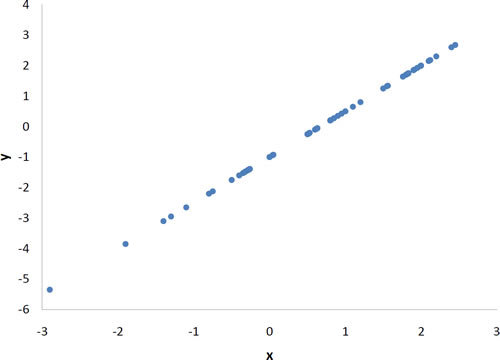
\includegraphics{pearson}
\end{figure}

PCA is another statistical procedure that transforms a set of data points using orthogonal transformation, which scales the set of points by a certain value, into a set of linearly uncorrelated values called principal components. Principal components are ordered such that the variance from the original variable decreases. It will always turn out that the first principal component will have the largest variance that was present in the original variable.

In machine learning, PCA is used to reduce the dimensionality of a set of data points. In implementing PCA on a 2D data set, the mean and the covariance of the data set would first have to be computed first. Mean is computed using $m = \frac{1}{P}\sum_{\mu=1}^{p} x^\mu$ and Covariance is measured using $S = \frac{1}{P-1}\sum_{\mu=1}^{P} (x^\mu-m)(x^\mu-m)^T$ (Storkey, 2017).

The eigenvalue and the eigenvector would also have to be computed. Eigenvector is computed using the formula $det(\lambda I - A ) = 0$, where $\lambda$ is the eigenvalue, I is the identity matrix of A, det is the determinant of the matrix, and A is the covariance matrix from the previous step. Eigenvalue is computed using the formula $( \lambda I - A )v = 0$.

For each data point $x^n$, the lower dimensional representation is $y^\mu = E^T(x^\mu - m)$ and the approximate reconstruction of the original data point $x^n$ is $x^\mu = m+Ey^\mu$. The total squared error over all the training data made is given by $(P-1)\sum_{j=M+1}^{N} \lambda j$ where $\lambda j , j = M + 1 . . . N$ are the eigenvalues discarded in the projection.

The last step is to choose the components and to form the feature vector. The number of eigenvectors and eigenvalues is equal to the number of data in the dataset. The eigenvector corresponding to the highest eigenvalue is the principal component of the dataset. To form the feature vector, the top k eigenvectors with top eigenvalues will be  used. To compute for the principal component, the transposed version of the feature vector is left-multiplied with the transposed version of the scaled version of the original dataset.

Fisher-like criterion makes use of the formula $\frac{m_0-m_1}{s_0-s_1}$, wherein m is the mean value of the feature for the$i$-th element and $s$ is the corresponding standard deviation. This algorithm can only be used, however, when dealing with binary classifications.

Feature selection, in general however, can be classified into three categories, namely the filter methods, wrapper methods, and the embedded methods. Filter method involves labelling each feature with a statistical measure and by comparing these measures, the more important features can be selected. Wrapper method involves grouping different combinations of features together to see which combinations work best. Embedded methods involve learning which features best contribute to the accuracy of the model while the model is simultaneously being created. Some more examples of feature selection algorithms would include best-first search, hill-climbing algorithm, and the usage of heuristics. Best-first search and hill-climb fall under the wrapper methods wherein different combinations are used until the top n features are found. Heuristics falls under the filter method wherein a heuristic score is given to each feature using a statistical measure such as Euclidean distance for example, and the features with the high scores will be the ones selected.

\section{Machine Learning}

Machine learning as defined by Ng (2017) is the science behind computers acting on a certain stimulus without being explicitly programmed to do so. Some examples of impact led by machine learning would be self-driving cars and web search suggestions from Google. Machine learning is also widely used in many different fields of research such as in artificial intelligence, data mining, natural language processing, image recognition, and expert systems (McCria, 2014). In machine learning, the concept of training the system to perform a unique task given a certain amount of data received has two main underlying categories, unsupervised learning and supervised learning.

\subsection{Supervised Learning}

Supervised learning, as defined by Brownlee (2016), is a type of machine learning wherein an input variable and an output variable is defined and an algorithm is used to map the input to the output variable. The goal of this type of learning is to map the input variables to their respective output variables by approximation so that when a new input variable is presented, an output can be predicted by the system. The main difference of supervised learning over unsupervised is that there is no third party that supervises and corrects the training of data in unsupervised but in supervised, intervention of the supervisor is necessary in order to achieve an acceptable level of performance by the system. Supervised learning can be further divided into two groups, namely regression and classification. Regression is used when the output is a real value, for example, weight, height, or age. Classification is used when the output is a category or group, for example, colors, sizes.

\subsection{Unsupervised Learning}

Brownlee (2016) defines unsupervised learning as having no corresponding output variable. Unsupervised learning is analysing the structure and distribution of the data in order for system to learn. Unsupervised learning can be further classified into two groups of algorithms, namely the clustering and the association. Clustering is used for discovering the groupings of data through clusters and association is used for discovering rules that describe the provided data.

\subsubsection{SOM}
Teuvo Kohonen (1995) defines SOM as a data visualization technique developed by Professor which reduces the dimension of data through the use of self-organizing neural networks. As SOM reduces the dimension of data, it also groups similar data items together; therefore, it not only reduces the dimension of data but also groups similar ones together. Figure 3.2 shows a basic example of a SOM. Note in this example that the data represented by colors are grouped according to their similarity (eg. yellow is near orange, dark teal is between blue and green).

\begin{figure}[h]
\caption{SOM Sample}
\centering

\includegraphics{som}
\end{figure}

Rumelhart \& Zipser (1985) defines a class under supervised learning called competitive learning. Here, neurons compete among themselves in a winner-takes-it-all scenario wherein only one neuron wins and is activated at any one time. Implementation of this competition is done through the use of lateral inhibition connections, which are structures of a network in which neurons inhibit their neighbors. When neurons are forced to organize themselves through this scenario, then the result would be a map that is self-organized, thus a SOM.

\subsubsection{K-Means Clustering Algorithm}

K-means clustering algorithm is a type of unsupervised learning algorithm wherein a set of unlabeled data will be grouped together and these groups are defined as the k variable. The algorithm will assign the different data points to their respective k-groups based on the selected features. Data points will then end up being clustered based on their feature similarities. The algorithm has two main iterative steps, , the data assignment step and the centroid update step, that repeats until either data points change clusters, the sum of the distances is minimized, or some maximum number of iterations is reached. Before starting with these two steps, the centroid for each k-cluster is computed first. In data assignment, each data point is placed in their nearest centroid value computed with squared Euclidean distance. In centroid update, the centroid is recomputed by taking the mean of all the data assigned to the cluster of the centroid (Hartigan \& Wong, 1979).

\subsubsection{t-SNE}

Maaten \& Hiton (2008) introduces t-SNE as a variant of the Stochastic Neighbor Embedding (SNE), which seeks to visualize high dimensional data by plotting these data points in a two or three dimensional map. Since t-SNE is a variant of SNE, SNE would have to be discussed first before transitioning to t-SNE. SNE starts by transforming the Euclidean distances of the high-dimensional data points into conditional probabilities that represent similarities. For example with $p_{j|i}$, this would represent the similarity from $X_j$ to $X_i$, that $X_i$ would pick $X_j$ as its neighbor if neighbors were picked in proportion to their probability density under a Gaussian centered at $X_i$. The conditional probability of $p_{j|i}$ is given with $p_{j|i} = \frac{exp(-||x_i-x_j||^2 /2 \delta_i^2}{\sum_{k \neq i} exp(-||x_i - x_k||^2 / 2 \delta_i^2}$ where $\delta i$ is the variance of the Gaussian that is centered in $X_i$. $p_{i|i}$ is set to 0 since only pairwise similarities will be considered. For the low dimensional counterpart of $X_i$ and $X_j$, the probability is computed by $q_{j|i} = \frac{exp(-||y_i - y_j||^2}{\sum_{k \neq i} exp(-||y_i - y_k||^2)}$.

As with its high dimensional counterpart, $q_{i|i}$ is set to 0. In order for SNE to find a low dimensional data representation that represents the mismatch between $p_{j|i}$ and $q_{j|i}$, a cost function is used, $C = \sum_{i} KL(P_i||Q_i) = \sum_{i}\sum_{j} p_{j|i} log \frac{p_{j|i}}{q_{j|i}}$,where KL is the Kullback-Leibler divergences, $P_i$ is the conditional probability distribution over all other data points given data point $X_i$, and $Q_i$ is the conditional probability distribution over all other data points given data point $Yi$.

With the variance $\delta i$  of the Gaussian that is centered over each high-dimensional data point $X_i$, it is important to note that the density of all data points in a data set are not uniform and it is more appropriate to use a smaller $\delta i$ value in denser regions than in sparser regions. Any value of $\delta i$ influences a probability distribution $P_i$ over all other data points. This probability distribution has an entropy value which increases as $\delta i$ increases. SNE seeks for a value of $\delta i$ that has a $P_i$ with fixed perplexity specified by the user using binary search. The perplexity is computed by $Perp(P_i) = 2^{H(P_i)}$ where the $H(Pi)$ or the Shannon entropy of $P_i$ is further computed using $H(P_i) = -\sum_{j} p_{j|i} log_2 p_{j|i}$. The smooth measure of the effective number of neighbors can also be identified as the perplexity and the typical values for this would range from 5 to 50. The cost function shown earlier can also be minimized into $\frac{\delta C}{\delta y_i} = 2\sum_{j} (p_{j|i} - q_{j|i} + p_{i|j} - q_{i|j})(y_i - y_j)$.

The gradient can be thought of as a spring force from a map point $y_i$ to any $y_j$ along the map. As the force is computed with $y_i-y_j$, the resulting force can either make the points repel or attract each other depending if the distance between the two is too small or too large. To speed up the optimization and to avoid poor local minima, a gradient update with a momentum term is done using $y^{(t)} = y^{(t-1)} + \eta \frac{\delta C}{\delta y} + \alpha (t) (y^{(t-1)}-y^{(t-2)})$ where $y^t$ indicates the solution at iteration t, $\eta$ indicates the learning rate, and $\alpha (t)$ represents the momentum at iteration t.

In t-SNE, certain issues such as the crowding problem, which is when too many data points get crowded in a map with a small number of dimension such as with 2D or 3D, are tackled by using a symmetrized version of the SNE cost function with more simple gradients and to use Student t-distribution instead of the Gaussian distribution when computing similarity between two low-dimensional points. The alternative cost function for a symmetrized SNE is $C=KL(P||Q) = \sum_{i}\sum_{j} p_{ij}log\frac {p_{ij}}{q_{ij}}$ where $p_{i|i}$ and $q_{i|i}$ are set to 0 just as in SNE and $p_{ij}$= $p_{ji}$ as $q_{ij}$= $q_{ji}$ since they constitute the symmetric property. $p_{ij}$ is computed using $p_{ij} = \frac{exp(-||x_i - x_j||^2 / 2 \delta ^2 )}{\sum_{k \neq 1}exp(-||x_k - x_l||^2 / 2 \delta ^2 )}$ and $q_{ij}$ using $q_{ij} = \frac{exp(-||y_i - y_j||^2)}{\sum_{k \neq 1}exp(-||y_k - y_l||^2)}$. In order to avoid having $p_{ij}$ with extremely small values which results from outliers, $p_{ij}$ is first set by $p_{ij} = \frac{p_{j|i} + p_{i|j}}{2n}$ so that $\sum_j p_{ij} > \frac{1}{2n}$ for all data points $x_i$. The gradient of symmetric SNE is computed using $\frac{\delta C}{\delta y_i} = 4 \sum_j (p_{ij} - q_{ij})(y_i - y_j)$.

In t-SNE, just as discussed above, Student t-distribution with one degree of freedom will take the place of Gaussian distribution as the heavy-tailed distribution in the low-dimensional map. $q_{ij}$ will now be computed using $q_{ij} = \frac{(1+||y_i - y_j||^2)^{-1}}{\sum_{k \neq 1} (1+||y_k - y_l||^2)^{-1}} $. A student t-distribution with one degree of freedom is used because it has the property $(1+||y_i - y_j||^2)^{-1}$  wherein it  approaches an inverse law for large pairwise distances in the low dimensional map. The resulting map representation of joint probabilities will make the map points invariant to changes in the scale of the map. Large clusters of points that are far apart will also interact just the same way as how an individual point would.

The gradient of the Kullback-Leibler divergence between P and the Student t-based joint probability distribution Q can be computed using $\frac{\delta C}{\delta y_i} = 4\sum_j (p_{ij} - q_{ij})(y_i - y_j)(1+||y_i - y_j||^2)^{-1}$. The resulting gradient from t-SNE will strongly repel dissimilar data points resulting in a visual image that clearly separates each data class as can be clearly seen in the t-SNE results in Appendix E as compared with the results from the other dimensionality reduction techniques used.

In their experiment set-up, they used a total of three data sets as was discussed back in Chapter 2 which includes the MNIST data set, the Olivetti faces data set, and the COIL-20 data set. They first used PCA to reduce the dimensionality of the data to 30 so that the computation of pairwise distances between data points would be faster and at the same time also suppresses the noise without severely distorting the distances between the data points. They then applied different dimensionality reduction techniques which includes Sammon mapping, Isomap, and LLE to compare the resulting visualization later on with the result of t-SNE. The results of each data set for each technique on the MNIST data set can be viewed in Appendix E. The coloring scheme in the visual images represent each class of data. The cost function parameter they used for their experiment was Perp = 40 for t-SNE, none for Sammon mapping, and k = 12 for Sammon mapping and Isomap.

Their results show that t-SNE overall had better visualization because the data classes are more distinct or separated than compared with the results from the other methods.  In general, t-SNE outperformed all the other dimensionality reduction techniques used in their research; however, the authors point out that t-SNE has three general weakness to consider. The first one is that it is unclear how t-SNE will perform on the more general task of dimensional reduction. In other words, if dimensionality is increased to more than 3, it is unclear whether t-SNE will still produce optimal visualization results. One way of addressing this problem is to optimize the Student t-distribution to have more than one degree of freedom. The second weakness is the curse of intrinsic dimensionality since t-SNE only reduces the dimensionality of data based on the local property of the data. Data sets that have high intrinsic dimensionality and an underlying manifold that is highly varying causes the local linearity of assumption on the manifold that t-SNE implicitly makes be violated; therefore, applying t-SNE to data sets with high intrinsic dimensionality can produce unreliable results. One way to address this problem is to perform t-SNE on a data representation obtained from a model that represents the highly varying data manifold efficiently in a number of non-linear layers. The last weakness is the non-convexity of the t-SNE cost function. Since the cost function of t-SNE is non-convex, several optimization parameters would first have to be chosen. The constructed solutions would then vary depending on the optimization parameter used each time from an initial random configuration of map data point. They explicitly point out however that the same choice of parameters can be used for different visualization tasks and the result would still be of similar

\section{Edit Distance Metric}
Edit distance quantifies how dissimilar two strings are by counting the minimum number of allowable operations required to transform one string to another. There are different definitions for edit distance, each of them using a different set of single-character operations.

\subsection{Levenshtein Distance}
Given two strings, a and b over a finite alphabet, the Levenshtein distance is the minimum-weight sequence of operations that transforms a into b. In 1966, Levenshtein defines a set of three edit operations. Insertion is the insertion of a single symbol. If $X=ab$, then inserting the symbol $c$ produces $acb$. Insertion can also be applied to an empty string, as denoted $\epsilon \rightarrow c$, using $\epsilon$ to denote the empty string. Deletion of a single symbol changes $acb$ to $ab (c \rightarrow \epsilon)$. Substitution of a single symbol $x$ for a symbol $y \neq x$ changes $acb$ to $adb (x \rightarrow y)$. The three operations have non-negative unit costs; however, substitution of a character by itself has zero cost.

The Levenshtein distance is mathematically defined as the distance between two strings is given by $lev_{a,b}(len(a),len(b))$ where $lev_{a,b}(i,j)$ is equal to $max(i,j)$ if $min(i,j) = 0$, otherwise you take the minimum of the three operation costs. $lev_{a,b}(i,j) = max(i,j),$	  $if min(i,j) = 0; otherwise, min(lev_{a,b}(i-1,j)+1), min(lev_{a,b}(i,j-1)+1), or$   $ min(lev_{a,b}(i-1,j-1)+1_{a_i\neq b_j})$

The distance between the first $i$ characters of $a$ and the first $j$ characters of $b$ can be computed by using the recursive definition above. $1(ai \neq bj)$ is the indicator function equal to $0$ when $ai = bj$ and equal to $1$ otherwise. The first element in the minimum function corresponds to the deletion operation, the second to the insertion operation and the third to match.

Levenshtein distance has several upper and lower bounds. The distance should be at least the difference of the sizes of the two strings and at most, the length of the longer string. The distance is zero if and only if the strings are equal. Lastly, the distance between two strings is no greater than the sum of their Levenshtein distances from a third string, which satisfies the triangle inequality.

The researchers implement Levenshtein distance using java-string-similarity, a Java library by tdebatty implementing different string similarity and distance measures. Here, the Levenshtein distance is computed using dynamic programming (Wagner-Fischer algorithm), which has a space requirement of $O(m)$ and runs in $O(m*n)$.

Marzal and Vidal (1993) proposed an algorithm that computes for the normalized edit distance that works in $O(m*n/sup$ $2/)$ time and $O(n/sup$ $2/)$ memory space, where $m$ and $n$ are the lengths of the strings under consideration, and $m>=n$. Their research shows that normalized edit distance consistently provides better results than regular edit distance and post-normalized edit distance.

\subsection{Damerau-Levenshtein Distance}
In relation to Levenshtein distance, Damerau-Levenshtein allows another edit operation, the transposition of two adjacent characters. The Damerau-Levenshtein distance between two strings a and b is given by $d_{a,b}(i,j)$, whose value is a distance between an initial substring of string $a$ and a $j$ symbol prefix of $b$. The function is recursively defined below.
$d_{a,b}(i,j) = max(i,j)$   $if min(i,j)=0,$ $min(d_{a,b}(i-1,j)+1,min(d_{a,b}(i,j-1)+1),min(d_{a,b}(i-1,j-1)+1)$,or $min(d_{a,b}(i-2,j-2)+1)$   if $i,j>1$ and $a_i = b_{j-1}$ and $a_i - 1$ = $b_j$; otherwise, $min(d_{a,b}(i-1.j)+1),min(d_{a,b}(i,j-1)+1)$,or $min(d_{a,b}(i-1,j-1)+1_{(a_i \neq b_j)})$.

Each recursive call matches one of the cases covered by the Damerau-Levenshtein distance. The first one corresponds to the delete operation, the second, to the insert operation, the third, to match or mismatch, depending on whether the respective symbols are the same, and the fourth, to the transposition of two adjacent symbols.

Damerau-Levenshtein can be implemented in two different ways, restricted and unrestricted. The restricted implementation is known as the Optimal String Alignment distance and the unrestricted implementation is what is commonly referred to as Damerau-Levenshtein distance.The main difference between the two implementations is that the Optimal String Alignment algorithm computes the number of edit operations under the restriction that no substring is edited more than once. Another key difference is that Optimal String Alignment algorithm is considered a true metric, since the triangle inequality does not hold, unlike the classic Damerau-Levenshtein.

The two algorithms are extensions of the Wagner-Fischer dynamic programming algorithm, which is also used in computing for the Levenshtein distance.

\subsection{Longest Common Subsequence}
Compared to the classic three-operation definition of edit distance, longest common subsequence only allows insertion and deletion. The Longest Common Subsequence (LCS) distance could also be equal to the Levenshtein distance when the cost of substitution is the double of the cost of an insertion or deletion. LCS simply gets the longest string that both string being compared to have. This can be accomplished via dynamic programming by simply appending to an initial empty string (main match) every time a match between the two strings is found. When a mismatch occurs, the loop is simply traversed without doing anything. If a succeeding match is found after the first match, a new temporary empty string is used to append the characters until a mismatch occurs. Then this temporary string will simply be compared to main match and whichever is longer will be the one stored in main match. The process is repeated until the end of both strings.

\subsection{Difflib Python Library}
Python has a built-in library called difflib which particularly provides classes and functions for sequence matching. They can be used to compare any types of sequences such as files, strings, patterns, etc. The SequenceMatcher class in difflib can be used to compare pairs of sequences of any type, as long as the elements are hashable (Python Software Foundation, 2018).

The algorithm used by the library dates back to Ratcliff and Metzener (1988)’s gestalt pattern matching wherein the basic algorithm is “to find the longest contiguous matching subsequence that contains no junk element.” The same concept is then applied to the left and to the right of the substring until a match that looks right to people is found.

\section{Visualization}
\subsection{Single Image}

Just as done in Azcarraga \& Flores (2016)'s research work and in Maaten \& Hiton (2008)'s t-SNE, visualization for the result of the SOM and t-SNE is projected in a single image. With SOM, the BMU or best matching unit, which will be explained further in section 3.5.1, represents the music trajectory of a certain 1 second music segment from the symphony. This sequence of BMUs make up the visual image representation of a certain symphony. A color coding scheme was also used to denote the time sequence of a certain music trajectory in the image, blue representing the start and going to red as the music progresses as shown in Figure 3.3. For t-SNE, sample visual images can be seen in Appendix E.

\begin{figure}[h]
\caption{SOM Image from SOMphony}
\centering
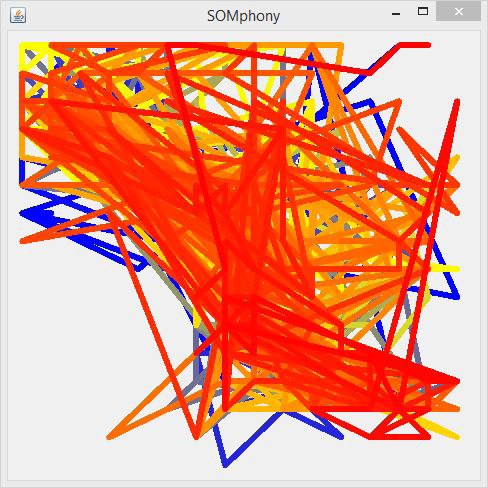
\includegraphics[width=0.5\textwidth]{somphony_sample}
\end{figure}

\subsection{Video}
Aside from representing the result of the SOM in a single image, it can also be represented in a video or multiple images. Video can be produced for the results of this research by collating  each 1 second segment result in order to show the progression of the musical trajectory grow from the start of the symphony to the end. This allows clearer visualization of the data to have more accurate analysis. Using this kind of visualization also greatly helps the survey user in the outcome of this research.

\subsection{3D Models}

In Azcarraga, Caronongan,  Setiono, \& Manalili (2016)’s research work, they incorporated the use of a structured 3D SOM instead of the regular SOM which will result in a single image. They represented the 3D map as a 3x3x3 dimensional cube with 27 subcubes each of the same sizes. Each subcube is further divided into 9x9x9 nodes. Here, they introduced the concept of a core cube at the center and the other 26 corresponding exterior cubes surrounding it. The training phase of the cube involved a four step labelling phase which was discussed in greater detail back in chapter 2. The resulting 3D SOM was then used to identify the proximity of a certain music to a particular genre. Each genre represented one corner of the cube as shown in Figure 3.4.

\begin{figure}[h]
\caption{3D SOM Cube}
\centering
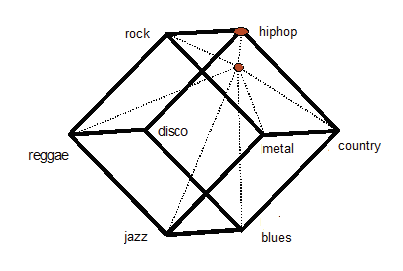
\includegraphics[width=0.5\textwidth]{cube}
\end{figure}

\section{Metrics}

There are two general types of data, qualitative and quantitative data. Qualitative data are data that cannot be measured by numbers while quantitative can be measured by numbers. Since this research will only make use of quantitative measurements, qualitative will no longer be discussed.

\subsection{Quantitative}

When using clustering as the method for machine learning, for example k-means clustering, there will result in k number of clusters after the algorithm is performed. Azcarraga \& Flores (2016) used k-means clustering in clustering the 1 second music segments. The best matching unit (BMU) for each 1 second music segment is first computed using Euclidean distance, which is the square root of the square of the difference between the x-axis of the first and second point added to the square of the difference between the y-axis of the first and second point, as shown in Figure 3.5.

\begin{figure}[h]
\caption{Euclidean Distance Diagram}
\centering
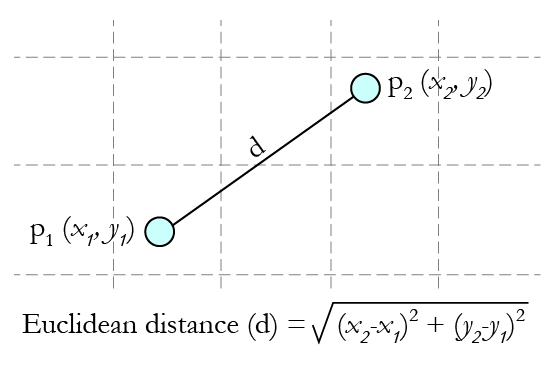
\includegraphics[width=0.5\textwidth]{euclidean}
\end{figure}

Each time a 1 second music segment has a BMU inside a cluster, the frequency count for that cluster is incremented. In this way, only the clusters that are mainly used by the music or symphony will have a high frequency count. The frequency counts are then normalized by dividing the counts of a certain composition by its total number of 1 second music segments. Once these normalized frequency counts are summarized, the resulting percentages can then be used to perform pair-wise comparisons between symphonies as shown in Appendix D.

\nocite{Dubnov}
\nocite{Azcarraga2016}
\nocite{cambouropoulosEmilios}
\nocite{3dsom}
\nocite{correa}
\nocite{imogen}
\nocite{libin}
\nocite{foote}
\nocite{silla}
\nocite{mcfee}
\nocite{hepokoski}
\nocite{heikkinen}
\nocite{bbc}
\nocite{huron}
\nocite{mckay}
\nocite{mcennis}
\nocite{loughran}
\nocite{lutter}
\nocite{mermelstein}
\nocite{agarwal}
\nocite{iitg}
\nocite{ng}
\nocite{mccria}
\nocite{brownlee}
\nocite{germano}
\nocite{bullinaria}
\nocite{kropotov}
\nocite{grabczewski}
\nocite{gupta}
\nocite{brownlee1}
\nocite{trevino}
\nocite{hartigan}
\nocite{brown}
\nocite{ziv}
\nocite{ron}
\nocite{mitchell}
\nocite{guyon}
\nocite{yang}
\nocite{kohonen}
\nocite{maaten}
\nocite{rumelhart}
\nocite{storkey}               %-- includes LaTeX source file for Chapter 3: Research Methodology
                                  %-- your job: **EDIT THIS FILE** to indicate your research methodology

%%%%%%%%%%%%%%%%%%%%%%%%%%%%%%%%%%%%%%%%%%%%%%%%%%%%%%%%%%%%%%%%%%%%%%%%%%%%%%%%%%%%%%%%%%%%%%%%%%%%%%
%
%   Filename    : chapter_3.tex 
%
%   Description : This file will contain your Research Methodology.
%                 
%%%%%%%%%%%%%%%%%%%%%%%%%%%%%%%%%%%%%%%%%%%%%%%%%%%%%%%%%%%%%%%%%%%%%%%%%%%%%%%%%%%%%%%%%%%%%%%%%%%%%%

\chapter{Research Overview}
This chapter contains procedures that propoenents will follow for the research based from theories and concepts discuess in chapter 3 and the methodologies discussed in chapter 1.

\section{System Architecture}

\begin{figure}[h]
\centering
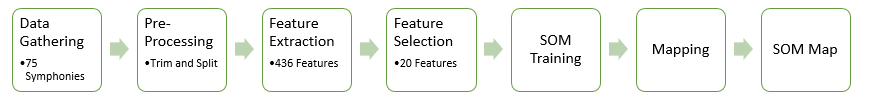
\includegraphics[scale=0.7]{sysarch1}
\end{figure}

\begin{figure}[h]
\centering
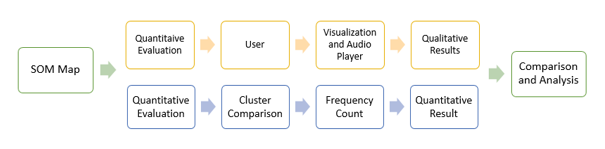
\includegraphics{sysarch2}
\end{figure}

\section{Preprocessing}

After acquiring the symphonies from online sources or through physical means, omitting segments of the music file which has no sound in it will be done using Audacity. This is done so that the output produced later will have no empty values since no sound will result in empty values. After the music files are cleaned, they will then be cut into one second music segments with a half second overlapping interval just as discussed in section 1.5.3 using Direct WAV MP3 Splitter. The music segments will then have their features be extracted using jAudio, producing an output file of XML. The XML file will then be converted to CSV format. The consolidated CSV file of all symphonies will then be used for feature selection to select only the more important features just as discussed in section 3.2.4. After the features have been selected, audio feature extraction will be done again, but only for these selected features. The resulting CSV file will then be used for machine learning using RapidMiner to be used in producing the SOM.

\section{Visualization Components}
\subsection{Function}

The program will allow the proponents to visualize the SOM in 3D by plotting the BMU of each music segment on a 2D plane and then collating the results of all segments in the composition in time series. The result is a line T(x, y, z) where (x, y) denotes the coordinates of the BMU of a particular music segment on the SOM and z being the index of the segment in the time series.

\subsection{Screenflow}

\begin{figure}[h]
\caption{Figure 4.1)}
\centering
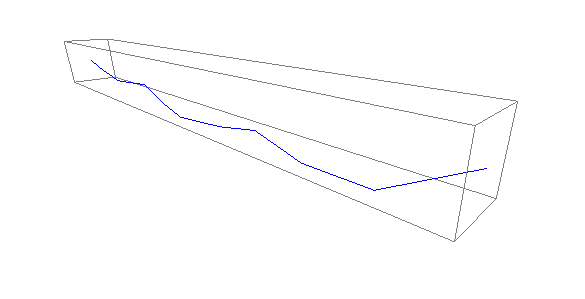
\includegraphics{visual1}
\end{figure}

Displaying the data of one symphony will plot a line that represents the musical trajectory or progression of the symphony in the SOM from start to finish. Each point on the z-axis (longest axis) represents the position of the BMU on the SOM at a particular interval in the time series as shown in Figure 4.1.

\begin{figure}[h]
\caption{Figure 4.2)}
\centering
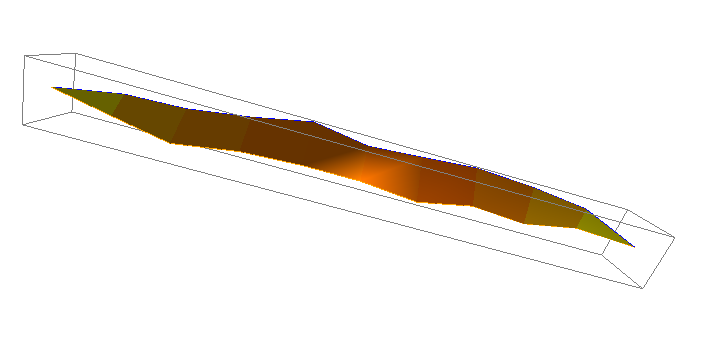
\includegraphics{visual2}
\end{figure}

Alternatively, when comparing two symphonies, two lines will be generated representing the musical trajectories of both symphonies. As shown in Figure 4.2, the area between the two lines will be colored depending on the Euclidean distance between the two BMUs in the same time axis.

\section{Testing and Methodology}
\subsection{Quantitative}

K-means clustering algorithm will be used as the algorithm for machine learning and Euclidean distance will be used for calculating the BMUs for each cluster to compare the similarities of symphonies just as discussed in section 3.5.1.

\subsection{Qualitative}

A survey form deployed online will be used to validate the result for the quantitative measurements starting April 2018 to June 2018. In the survey, the participant will first be asked for their voluntary consent as shown in Appendix E. Then, upon consenting, they will be asked to listen to two symphonies that are found to be similar using the quantitative measure used in the research as seen in figure 4.3. The system will provide suggested time slices for them to annotate. An annotation module is provided for the user to rate the similarity from 1 to 5, with 1 being dissimilar and 5 as similar. They may also choose to annotate which part/parts in the symphony that was not suggested yet they believe were similar. Upon selecting time slices, the coloration of the time slices would change depending on the \% similarity of the selected slice. A spectrum of red to green would be used, with red representing a low \% similarity and green representing a high \% similarity. The results from these should help validate if this research work’s methodology and speculated results prove true.

\begin{figure}[h]
\caption{Figure 4.3)}
\centering
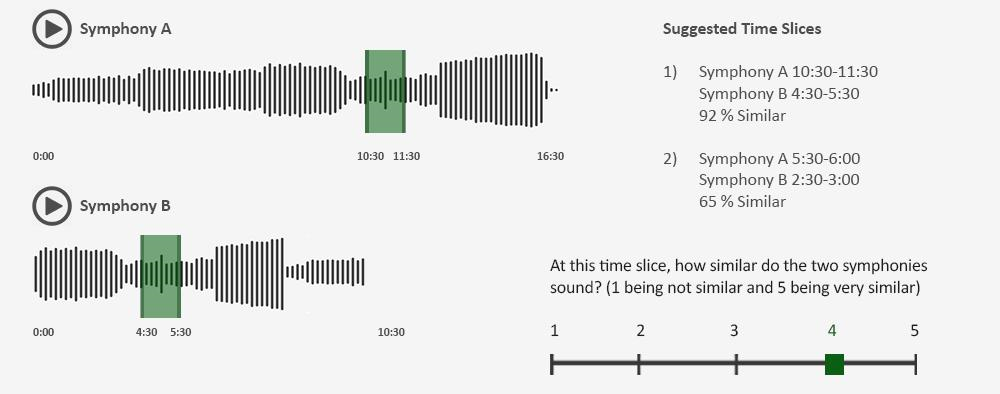
\includegraphics[scale=0.5]{survey}
\end{figure}

50 participants will be asked to answer these survey forms. The participants’ profile will come in the form of either musical inclined people or just regular people who may not know much about music. An estimate of around 60\% of the survey forms must be answered by musical inclined people and about 40\% answered by regular people because musical inclined people know best about music and are reliable sources for comparison but they may also hold biases with regards to the music they listen to or whether they like listening to this particular composer or not; therefore, including regular people in the survey will help lessen the bias since no knowledge over something will result in no bias. 

%%%%%%%%%%%%%%%%%%%%%%%%%%%%%%%%%%%%%%%%%%%%%%%%%%%%%%%%%%%%%%%%%%%%%%%%%%%%%%%%%%%%%%%%%%%%%%%%%%%%%%
%
%   Filename    : chapter_3.tex 
%
%   Description : This file will contain your Research Methodology.
%                 
%%%%%%%%%%%%%%%%%%%%%%%%%%%%%%%%%%%%%%%%%%%%%%%%%%%%%%%%%%%%%%%%%%%%%%%%%%%%%%%%%%%%%%%%%%%%%%%%%%%%%%

\chapter{Results and Analysis}
This chapter contains all the results from the research conducted and the corresponding analyses for the results.

\section{t-SNE Visualization Results}
After t-SNE was applied on the dataset as was discussed in Chapter 4, the resulting points were plotted according to different categories. For the entire set of t-SNE plots, please refer to Appendix F.

\subsection{Per Period Plot}
Figure 5.1 shows the plots for different musical periods. Each of the colors represent a different composer in each period:  blue for composer 1, green for composer 2, red for composer 3, purple for composer 4, and yellow for composer 5. All five periods had a similar shape of a ball since all of them represents an entire period of music and it would only be appropriate that the points are evenly scattered in the plane. Baroque period, however, has an obvious lack of plotted points in the figure compared to the others since this period in particular had the lowest number of data points originally due to the fact that the symphonies from here are generally shorter in time span. 20th Century, on the other hand, shows a more concentrated ball shape as opposed to others since this period had symphonies that are generally longer than that of other periods.

\begin{figure}[!htb]
\caption{Per Period Plot}
\centering
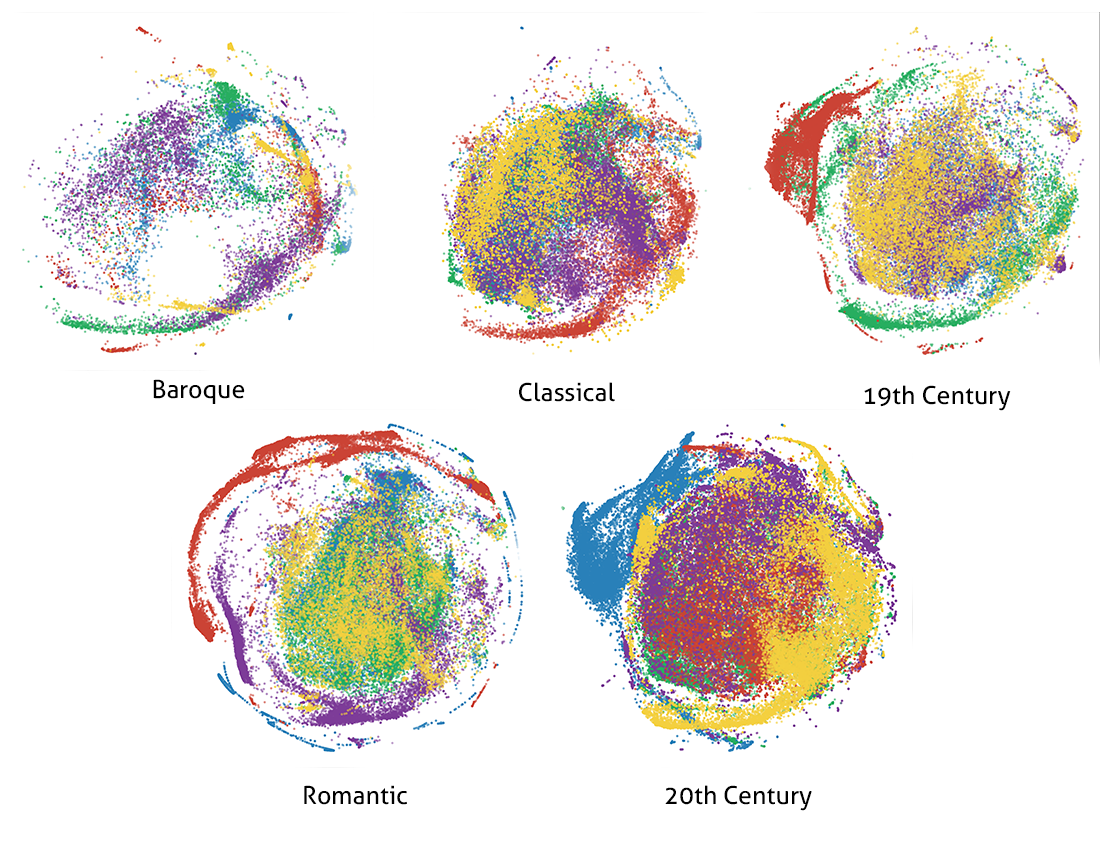
\includegraphics[scale=0.5]{per_era}
\end{figure}

\subsection{Per Composer Plot}
Figure 5.2 shows the plots of the different composer through each period. The first row of plots are from the Baroque Period, then plots from the Classical, 19th Century, Romantic and 20th Century Periods respectively.

\begin{figure}[!htb]
\caption{Per Composer Plot}
\centering
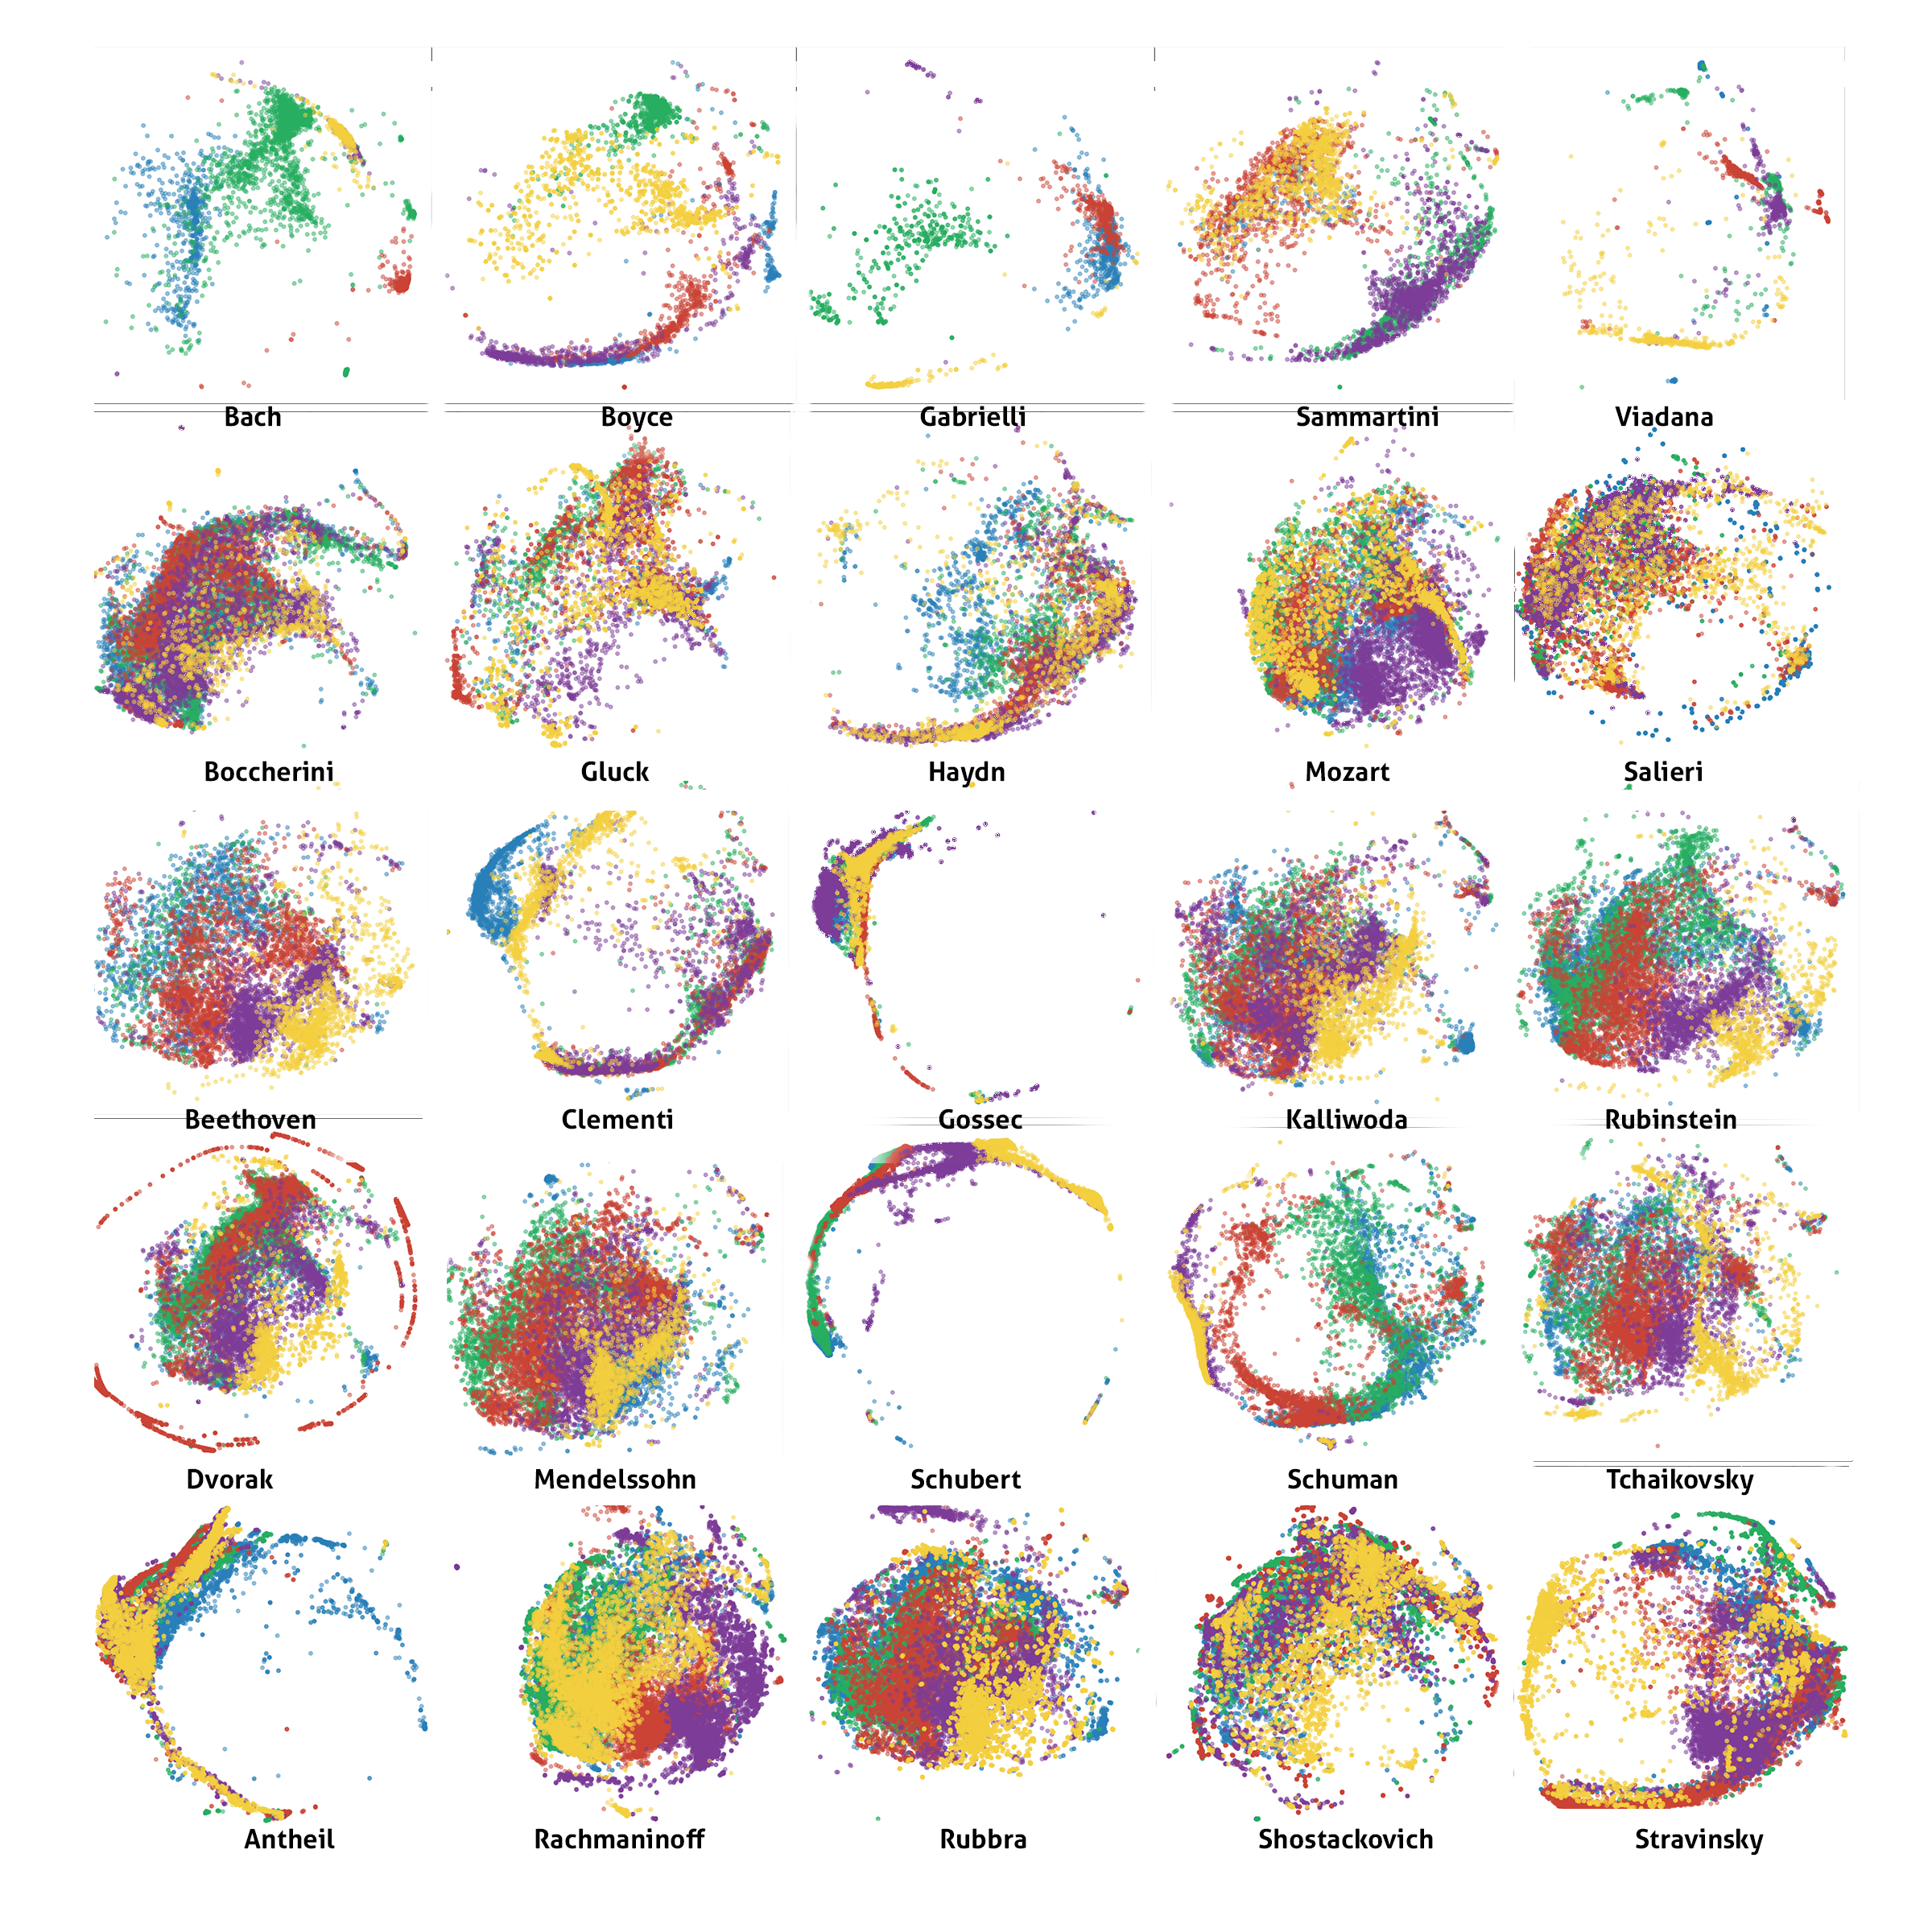
\includegraphics[scale=0.25]{per_composer}
\end{figure}

\subsection{Per Symphony Plot}
In order to represent the time-series aspect of the visualization, the researchers color graded the plotted points as the points aged. The colors span from yellow to green, to blue and to violet, from start to end respectively. An example of this gradation can be seen in Figure 5.3, which is the plot of (P5C2S5).

\begin{figure}[!htb]
\caption{Symphony Plot}
\centering
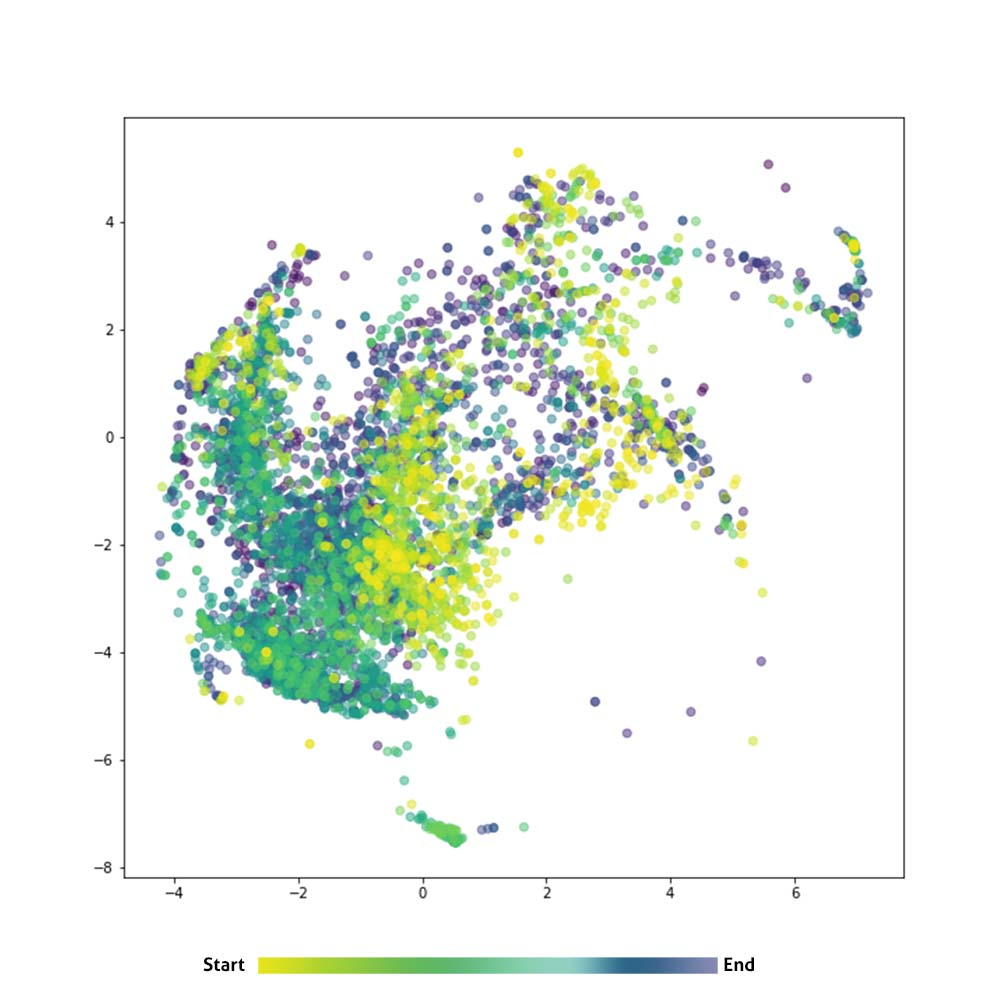
\includegraphics[scale=0.4]{Untitled-2}
\end{figure}

The gradation is done to all symphonies and is grouped and presented by music period. Figures 5.4 to 5.8 show the plots of each symphony as it progresses through time. 

\begin{figure}[h]
\caption{All Symphonies Part 1}
\centering
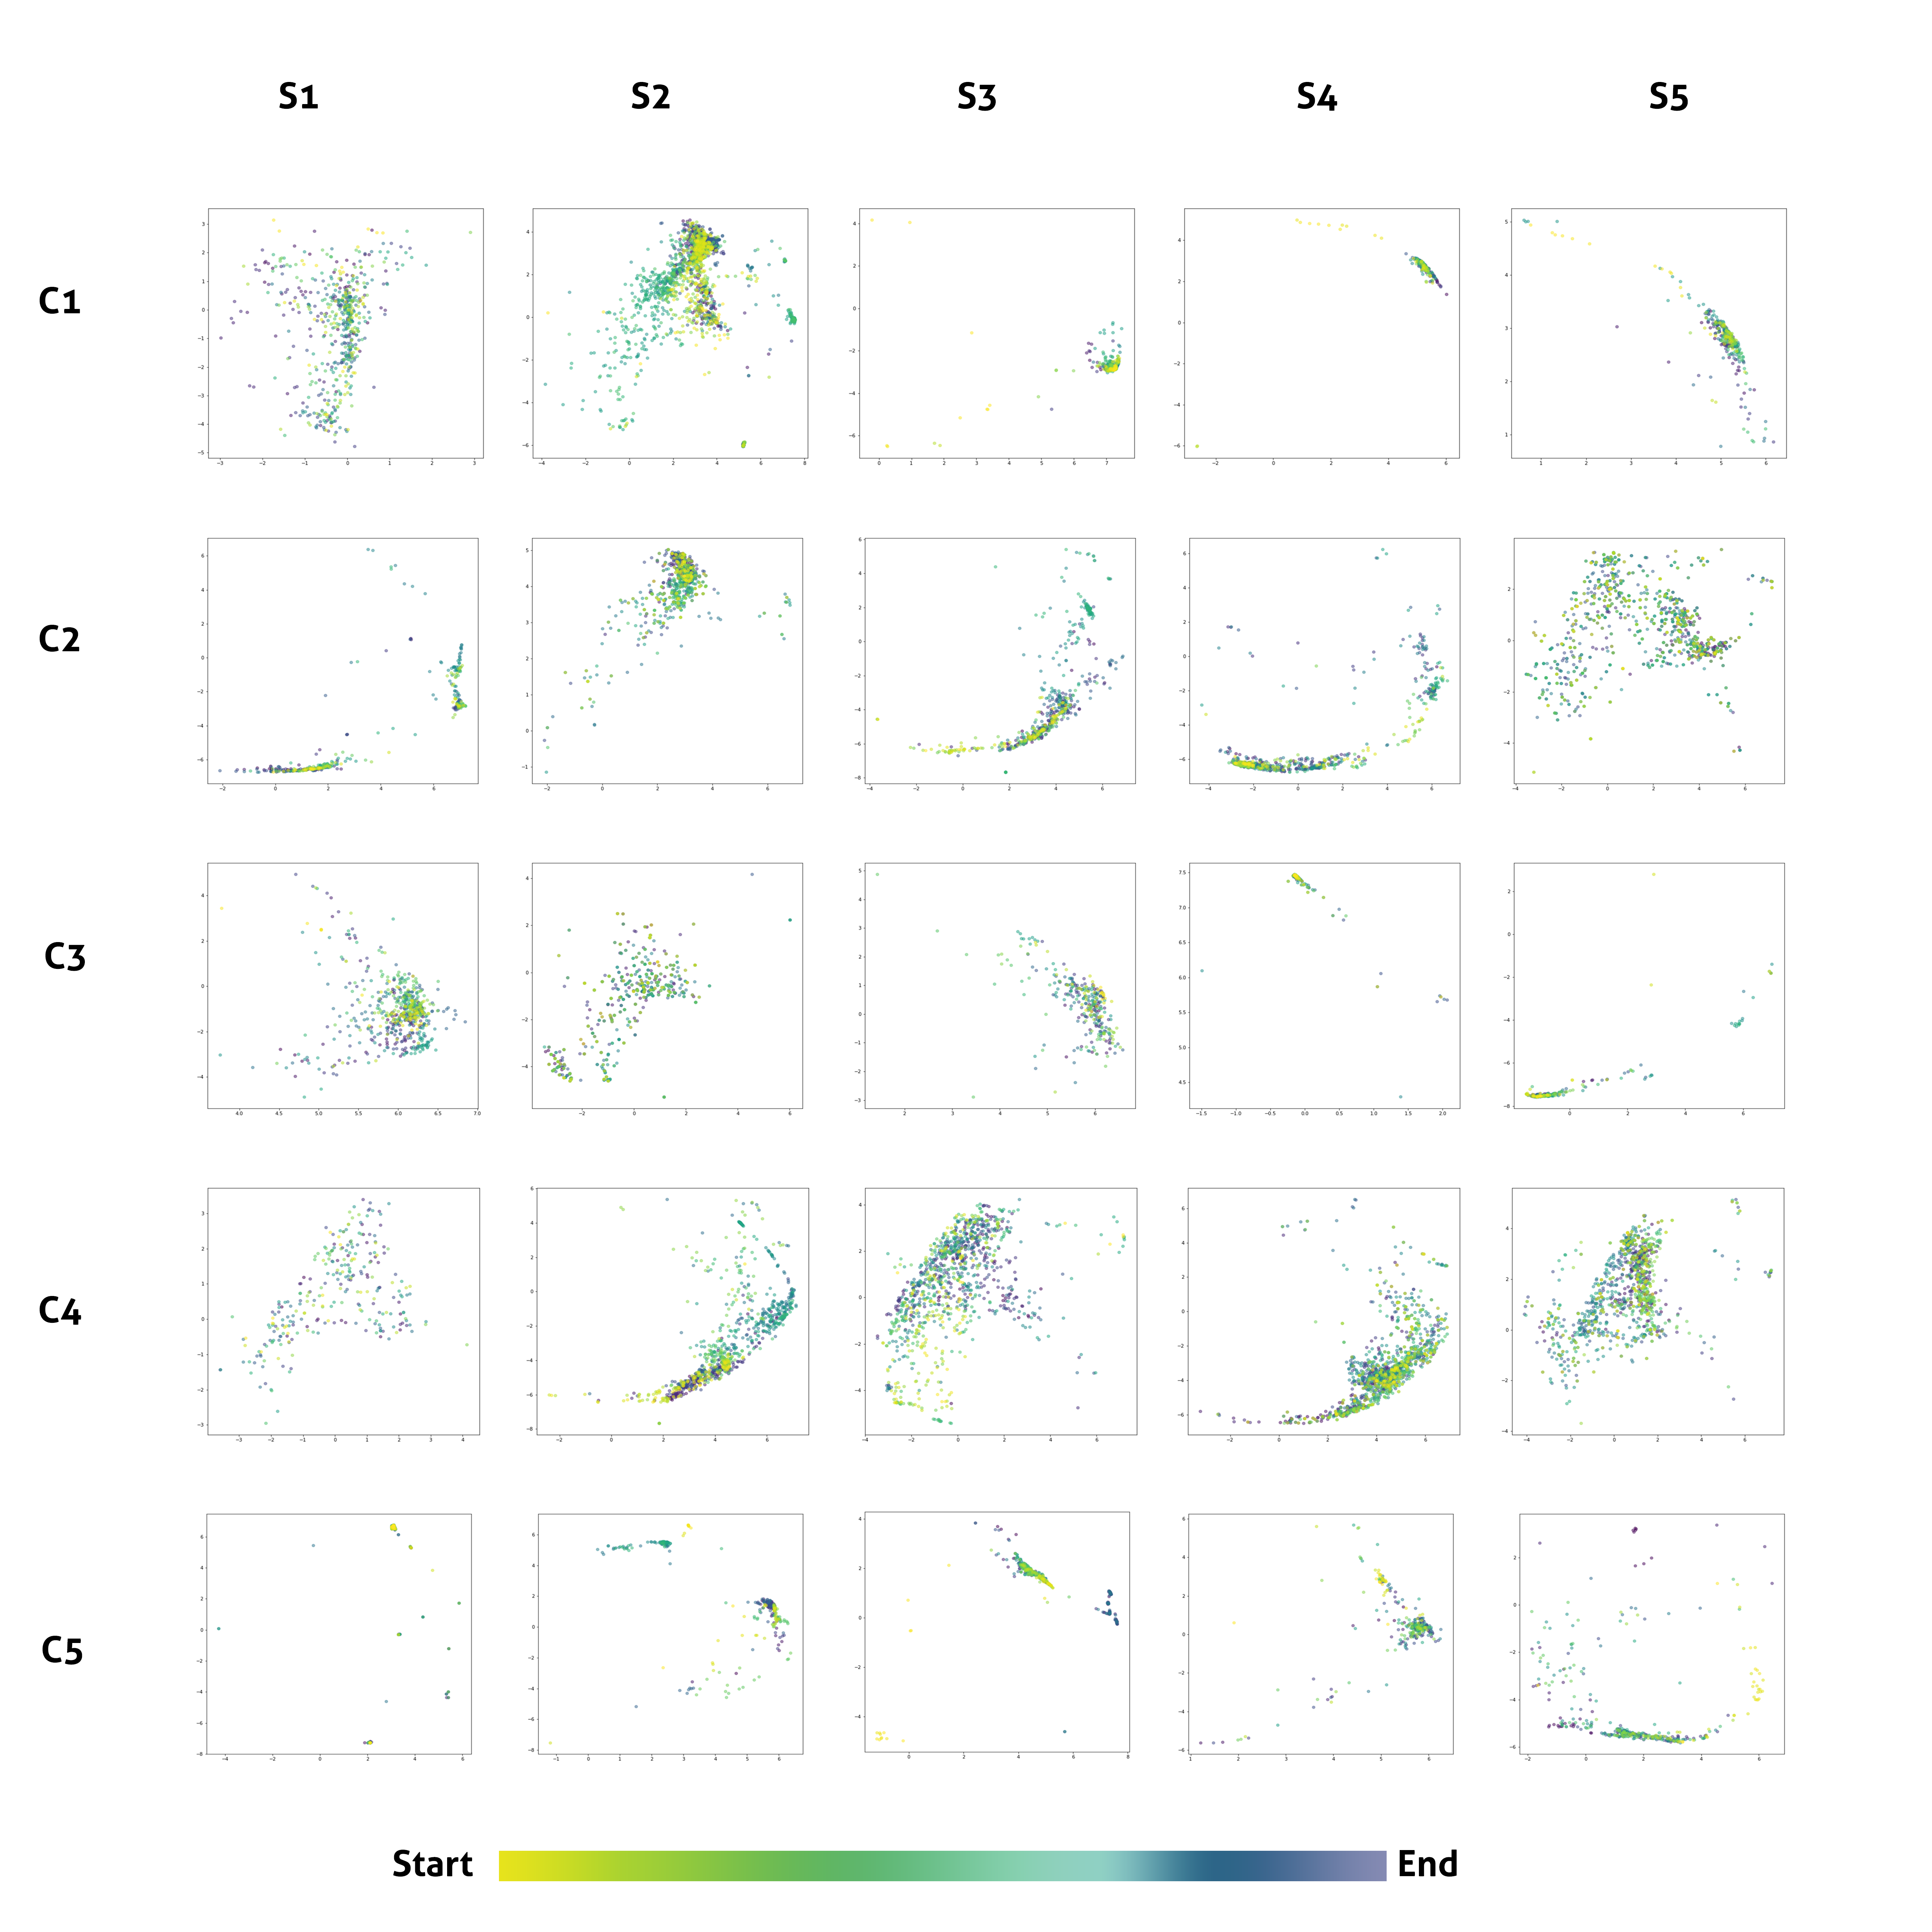
\includegraphics[scale=0.08]{p1-2_allsymphonies}
\end{figure}

\begin{figure}[h]
\caption{All Symphonies Part 2}
\centering
\includegraphics[scale=0.08]{p2_allsymphonies}
\end{figure}

\begin{figure}[h]
\caption{All Symphonies Part 3}
\centering
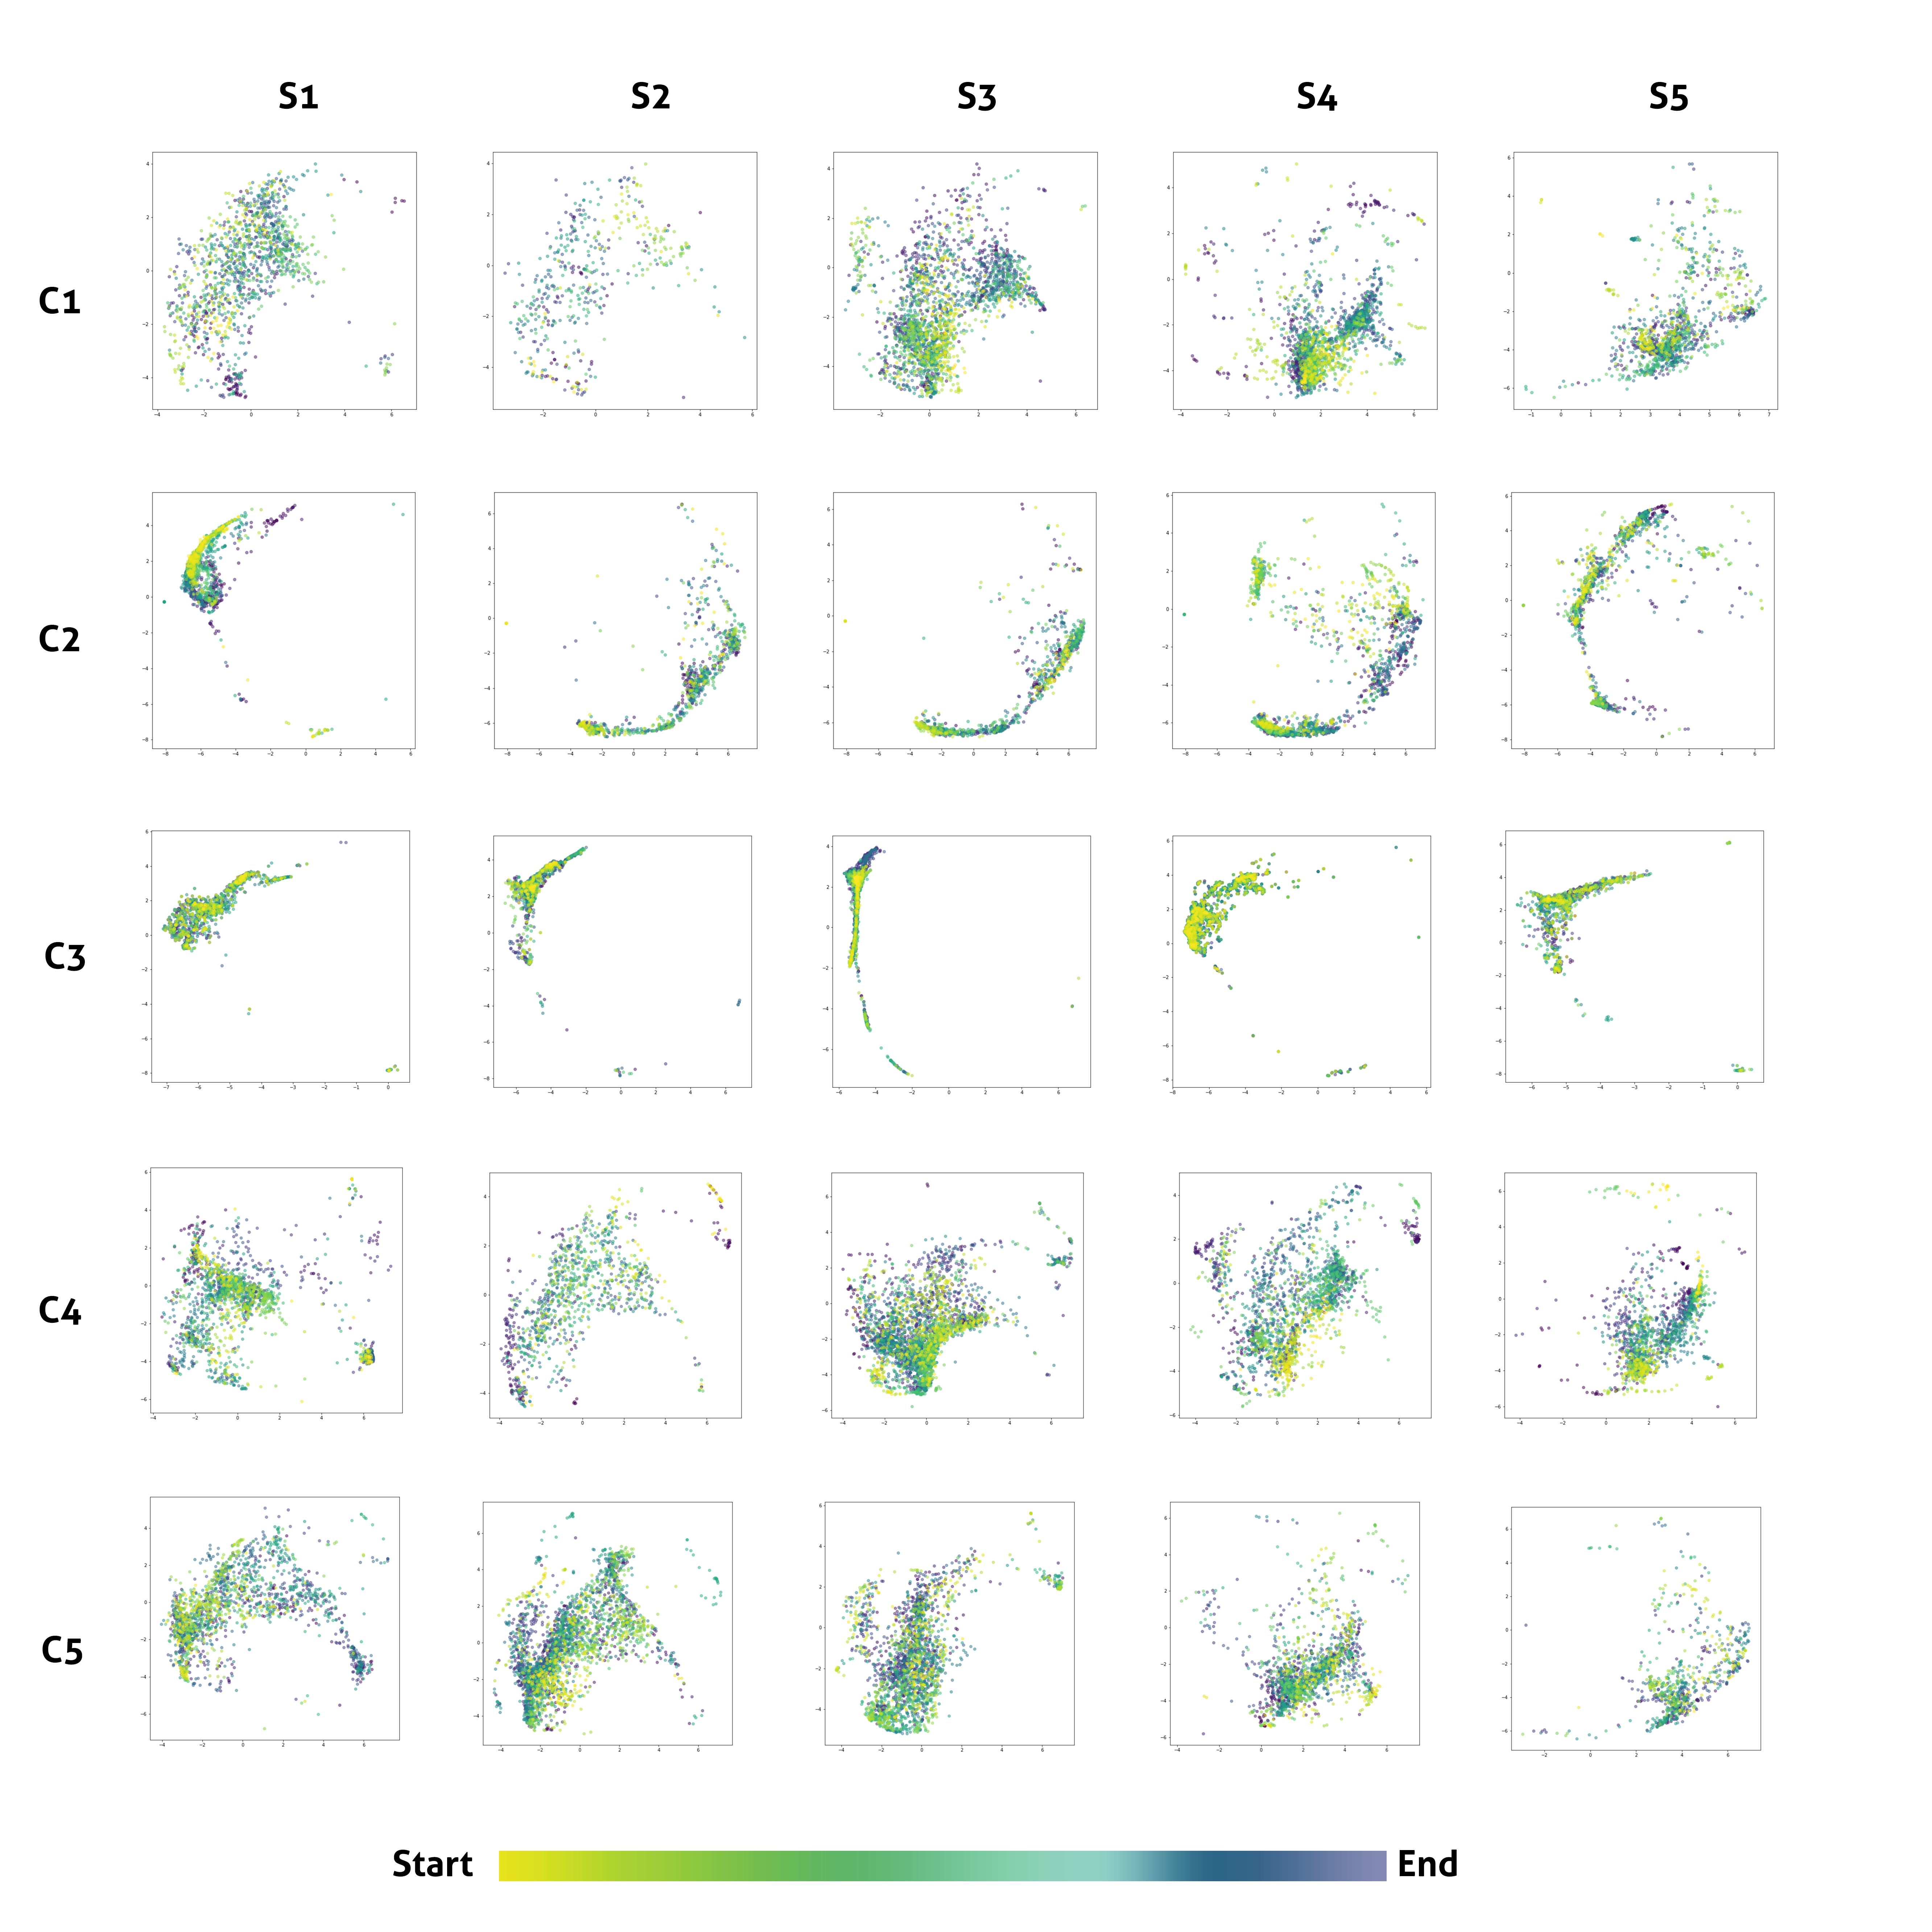
\includegraphics[scale=0.08]{p3_symphonies}
\end{figure}

\begin{figure}[h]
\caption{All Symphonies Part 4}
\centering
\includegraphics[scale=0.08]{p4_allsymphonies}
\end{figure}

\begin{figure}[h]
\caption{All Symphonies Part 5}
\centering
\includegraphics[scale=0.08]{p5_allsymphonies}
\end{figure}
\section{Qualitative Analysis}
Based on the t-SNE results of the 5 composers in the Baroque period, the researchers noticed that the points are not that scattered and forms an arc like shape. Each composer in the Baroque period have points that are located near each other especially Boyce and Sammartini. The other 3 composers in the Baroque period are parts of the pattern that the Boyce and Sammartini produced.  This result may suggest that composers in the Baroque period have similar styles of composition. In the graph of the 5 Classical composers, the points also form a similar pattern except for 1 composer, Haydn. The consistency and the solidness of the points are more noticeable in the Classical period compared to the Baroque Period. In the 19th Century Period, the results are a bit scattered throughout the map and composers Clementi and Gossec are noticeably having their own pattern. The other 3 composers of the 19th Century are the ones that created a similar pattern. This results in the 19th Century suggests that composers during this time have their own style of compositions, within the 5 composers of the 19th Century. In the Romantic Period, the graph resulted in a more diverse pattern of each composers compared to the 19th Century. There is no specific pattern or style that was shown in the graph that could determine the style of the Romantic Period composers. The same goes with the 20th Century, various styles are shown in the graph. In the earlier Periods like Baroque and Classical, more consistent and similar pattern styles are observable. This analysis suggests that early composers tend to have similar styles in composing symphonies. Through time, composers in the 19th Century, Romantic, and 20th Century period are more unique in terms of the way they compose their symphonies.

In terms of transition, the researchers noticed that the most number of similar graphs, visually looking, are present in all periods but are more dominant in the periods of Classical, 19th and 20th Century Composers. An example is the compositions of Mozart, wherein his graph has a similar pattern with 19th Century composers Beethoven, Kalliwoda and Rubinstein. This pattern continues to be present in the works of the Romantic period composers Mendelssohn and a little bit of Tchaikovsky. Lastly, the trend continues in the 20th Century composers Rachmaninoff and Rubbra. The pattern described throughout the periods is observed as a round shape style. Shown below is the development of the pattern that rooted in the composition of Mozart.

\begin{figure}[h]
\begin{minipage}{.5\textwidth}
  \captionof{figure}{Classical: Mozart}
  \centering
  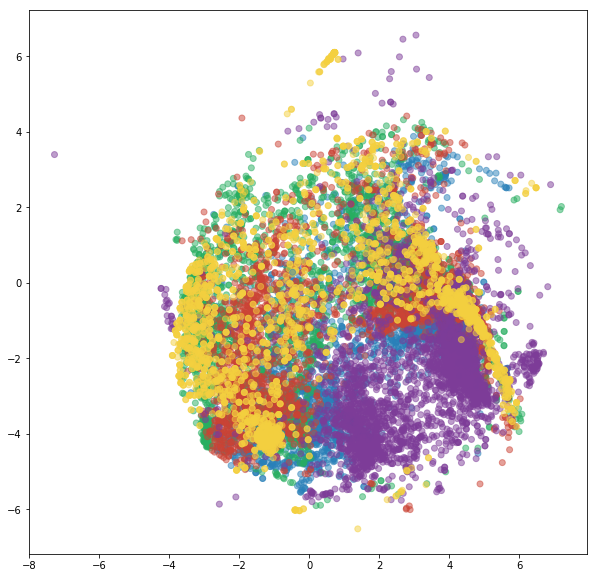
\includegraphics[scale=0.15]{P2C4}
  \label{fig:test2}
\end{minipage}
\end{figure}

\begin{figure}[h]
\begin{minipage}{.5\textwidth}
  \captionof{figure}{19th Century: Kalliwoda}
  \centering
  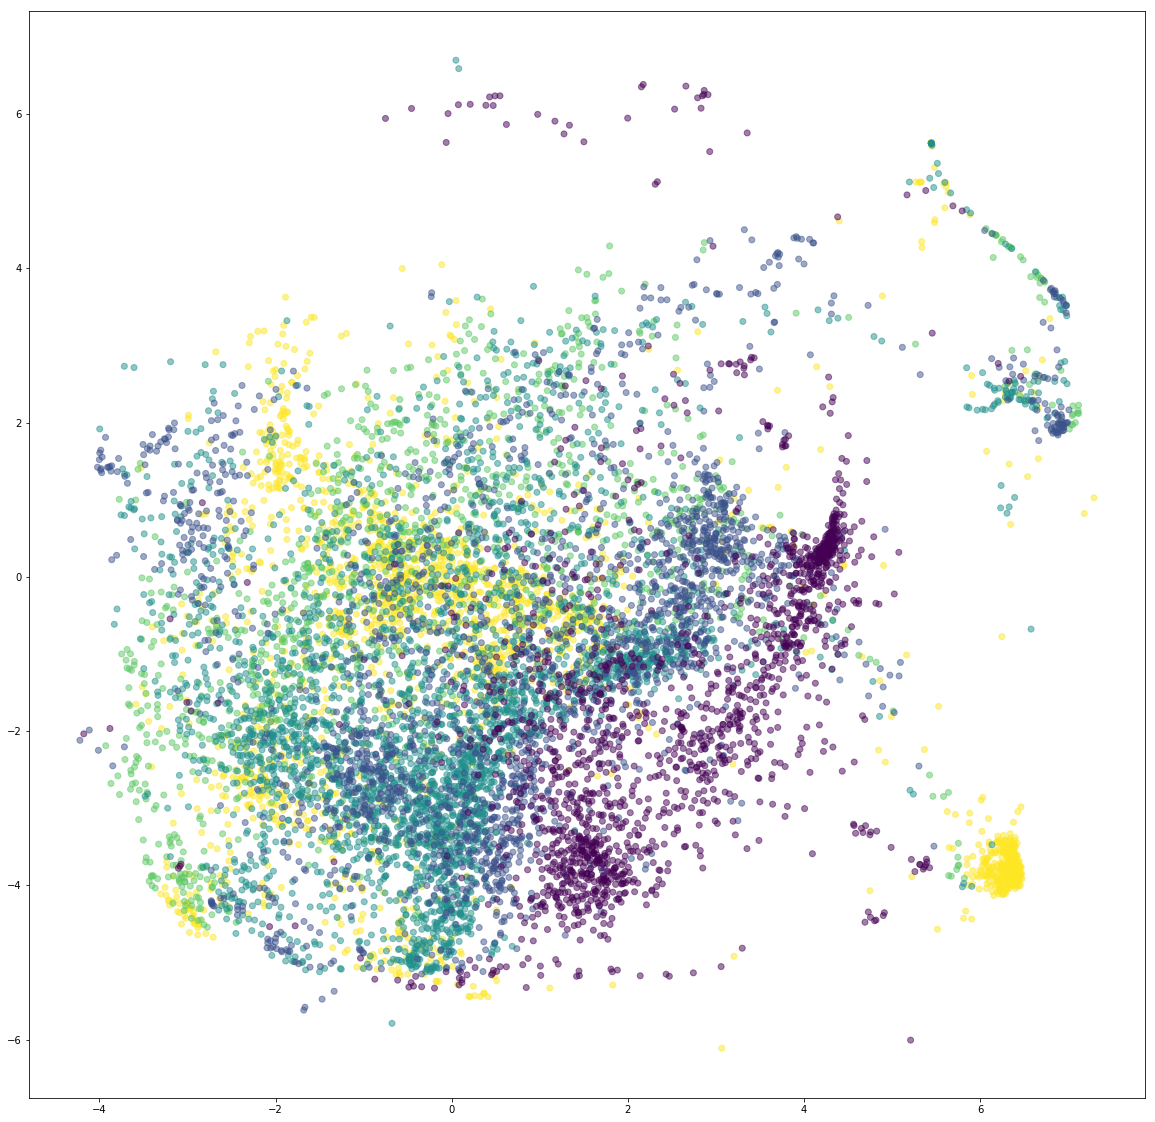
\includegraphics[scale=0.15]{P3C4}
  \label{fig:test2}
\end{minipage}
\begin{minipage}{.5\textwidth}
  \captionof{figure}{19th Century: Beethoven}
  \centering
  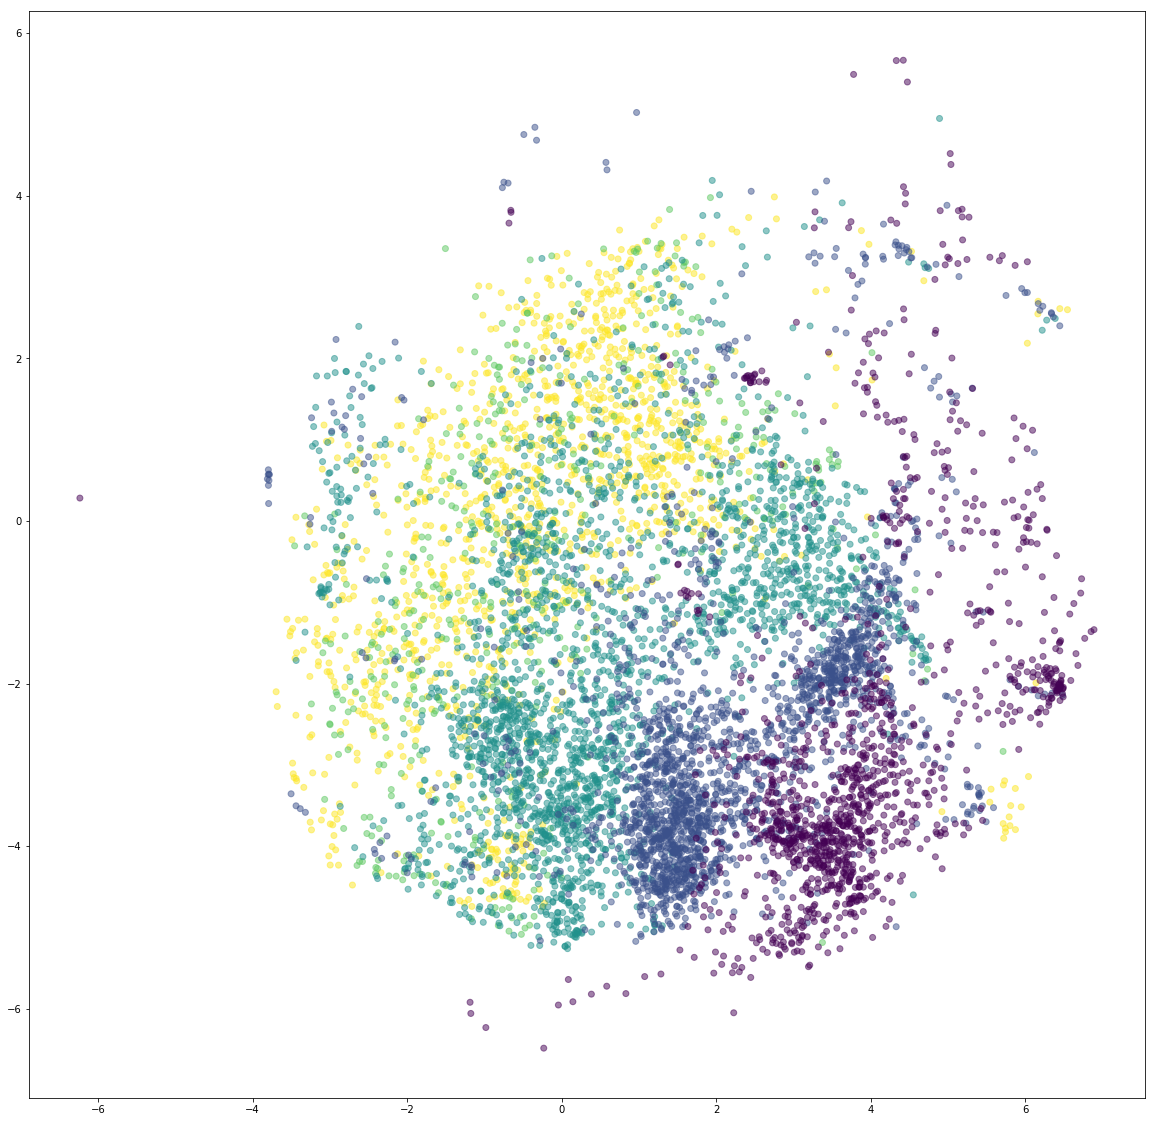
\includegraphics[scale=0.15]{P3C1}
  \label{fig:test1}
\end{minipage}
\end{figure}

\begin{figure}[h]
\begin{minipage}{.5\textwidth}
  \captionof{figure}{Romantic: Mendelssohn}
  \centering
  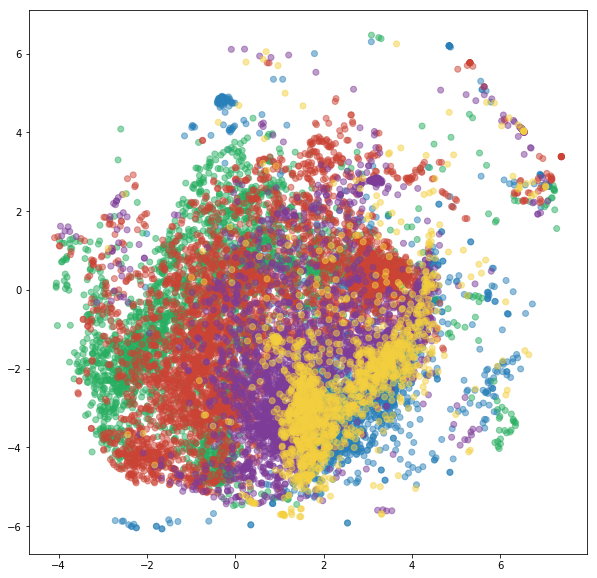
\includegraphics[scale=0.15]{P4C2}
  \label{fig:test2}
\end{minipage}
\begin{minipage}{.5\textwidth}
\caption{Romantic: Tchaikovsky}
\centering
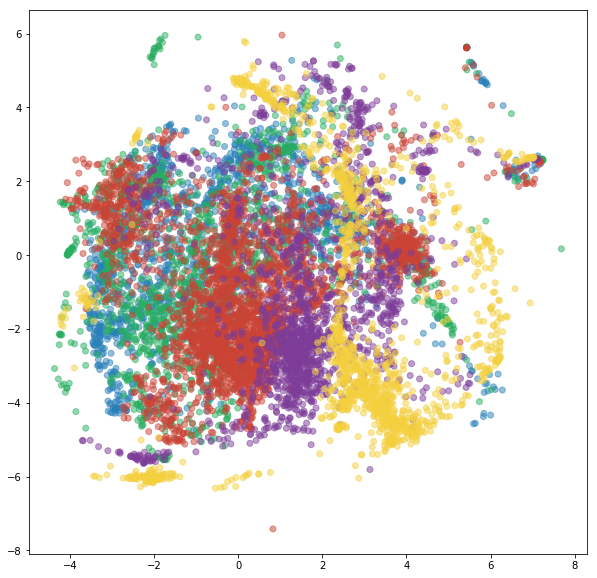
\includegraphics[scale=0.15]{P4C5}
 \label{fig:test3}
\end{minipage}
\end{figure}

\begin{figure}[h]
\begin{minipage}{.5\textwidth}
  \captionof{figure}{20th Cen: Rachmaninoff}
  \centering
  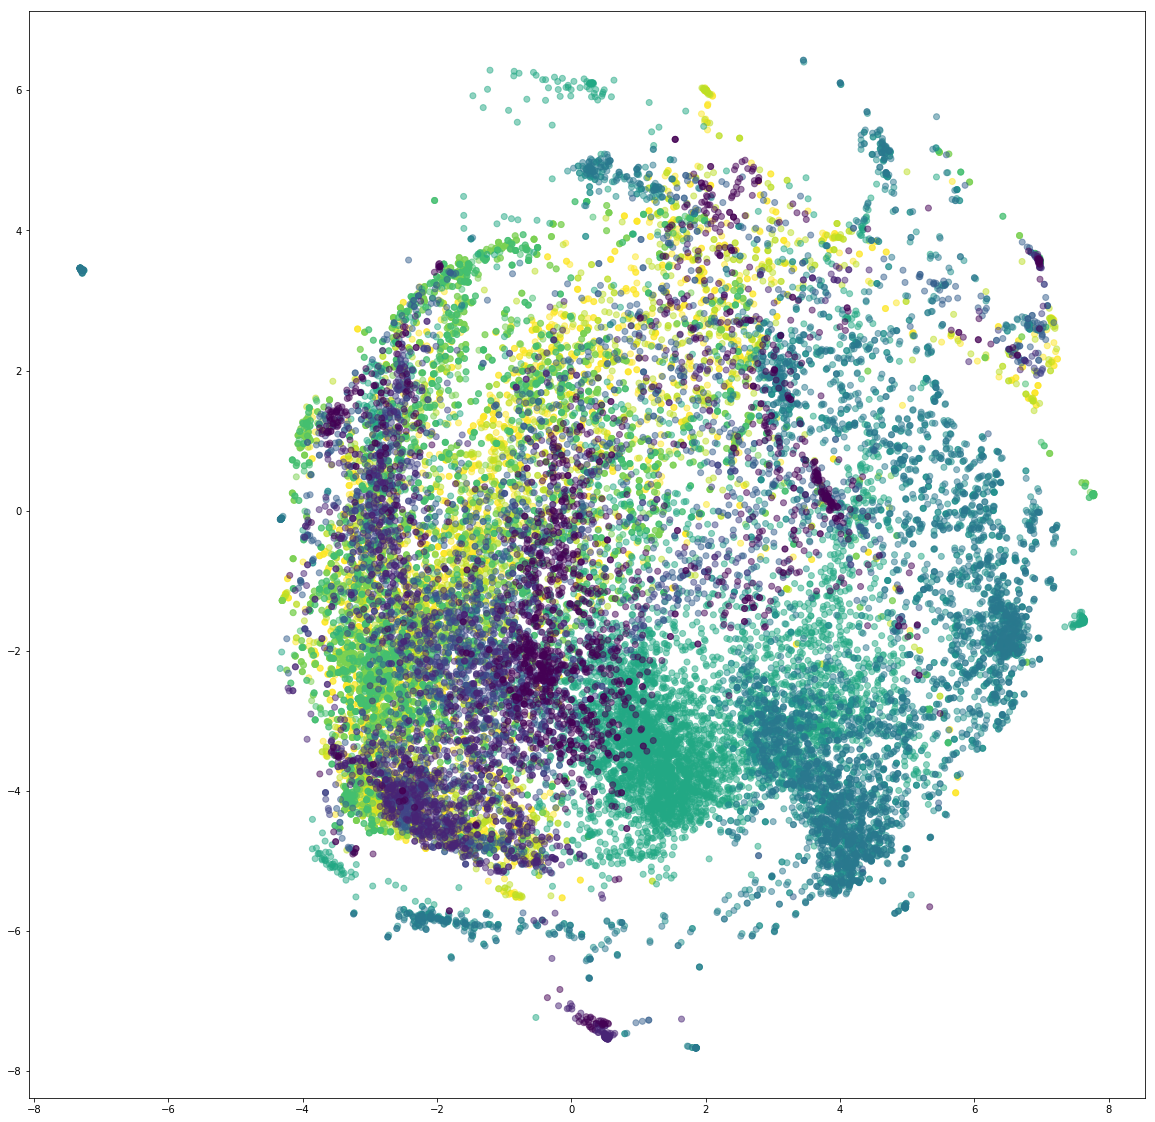
\includegraphics[scale=0.15]{P5C2}
  \label{fig:test2}
\end{minipage}
\begin{minipage}{.5\textwidth}
  \captionof{figure}{20th Cen: Rubbra}
  \centering
  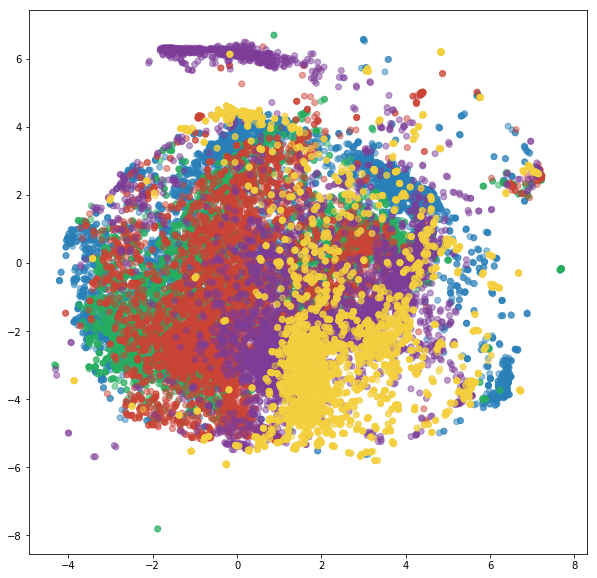
\includegraphics[scale=0.15]{P5C3}
  \label{fig:test1}
\end{minipage}
\end{figure}

\begin{figure}[h]
\caption{19th Century: Rubinstein}
\centering
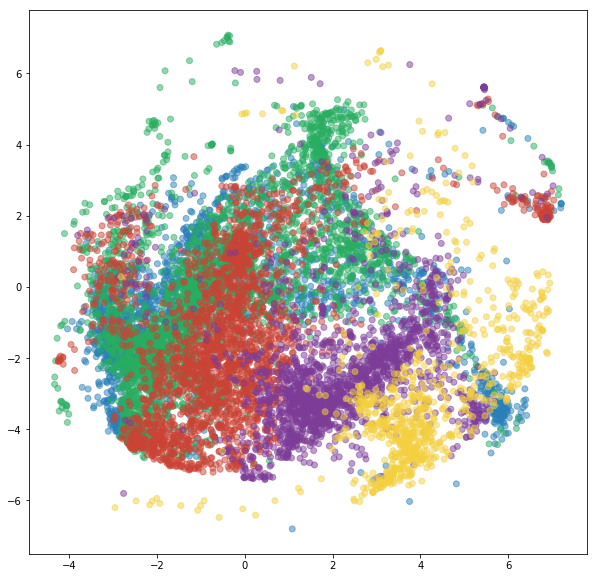
\includegraphics[scale=0.15]{P3C5}
\end{figure}
Another pattern that the researchers noticed is between the composers of the Barque, Classical and 19th Century. A unique pattern was observed to these two Baroque composers Boyce and Sammartini. Both composers have the most similar pattern in the Baroque Period as shown below.

\begin{figure}[!htb]
\begin{minipage}{.5\textwidth}
  \captionof{figure}{Baroque: Boyce}
  \centering
  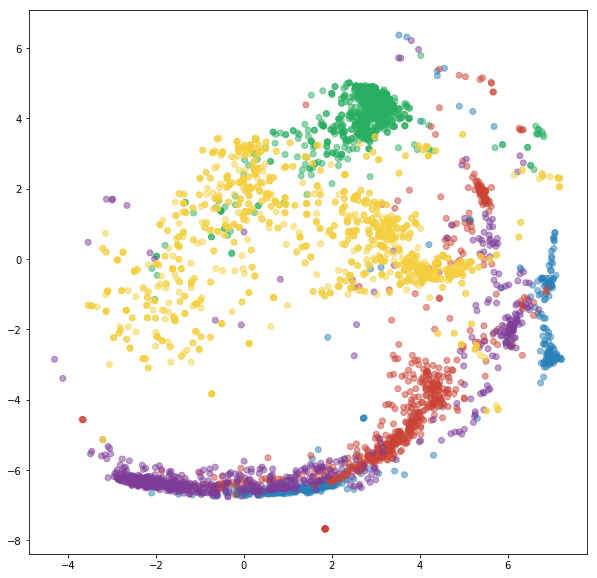
\includegraphics[scale=0.15]{P1C2}
  \label{fig:test2}
\end{minipage}
\begin{minipage}{.5\textwidth}
  \captionof{figure}{Baroque: Sammartini}
  \centering
  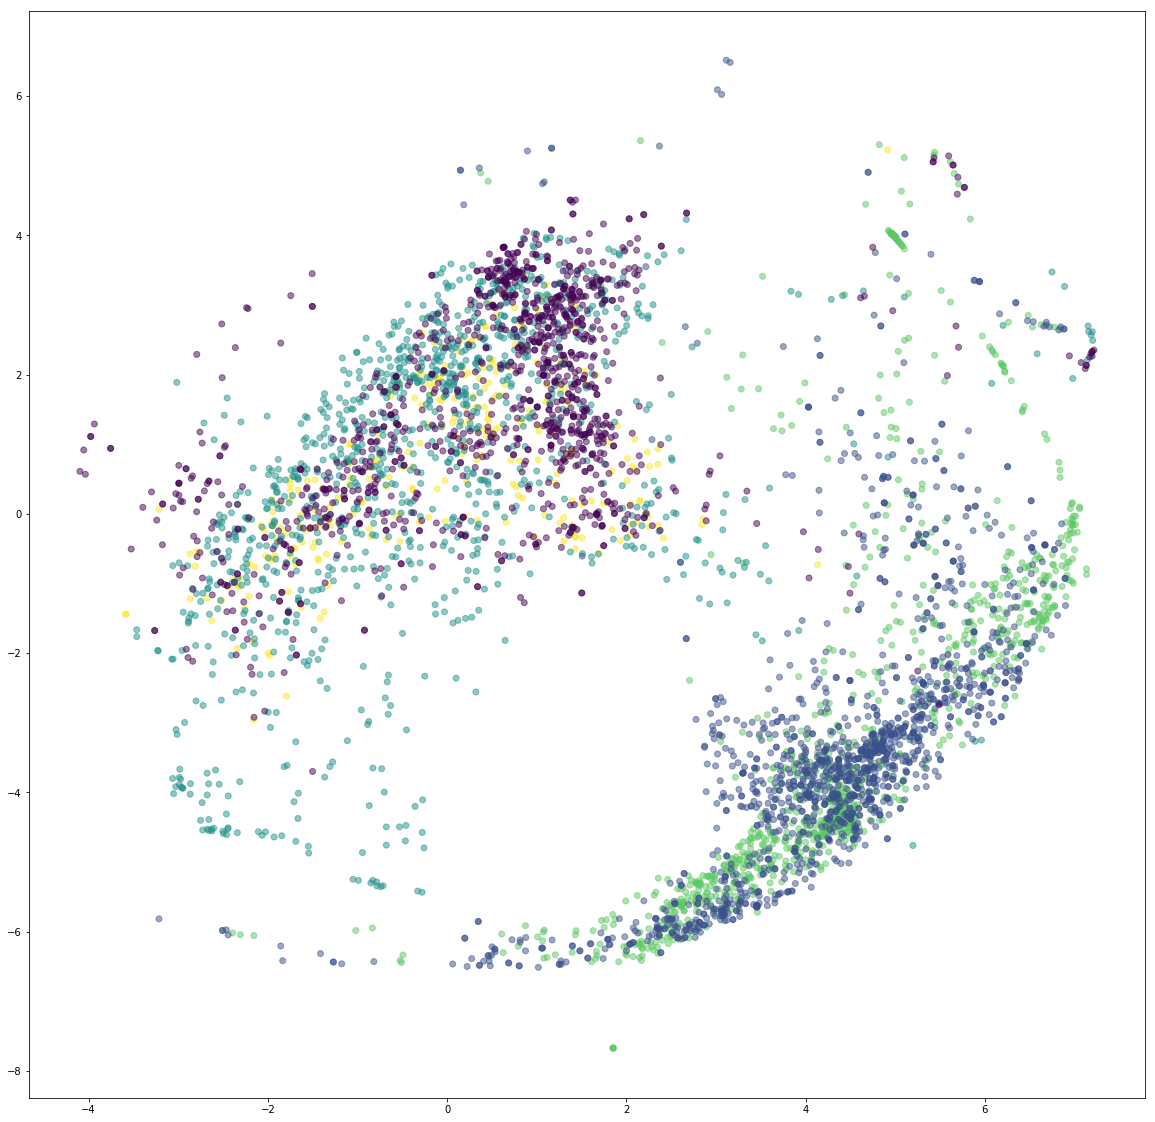
\includegraphics[scale=0.15]{P1C4}
  \label{fig:test2}
\end{minipage}
\end{figure}

In the Classical Period, composer Haydn had the same pattern except on the top left part of the graph. The research considered that the pattern of Haydn is still relevant or influenced by the Baroque composers because the left and bottom part of the graph is similar. Two of Haydn’s are the ones that influence the change of the graph in comparison to the Baroque composers. The graphs of the said composers would be more similar without the two works of Haydn. Moving on to the Classical period, the trends was observe to be present in the works of Clementi. Just like Haydn’s, the same top left area is the main difference compared to the Baroque composers that was also caused by two of his compositions. Without the blue and yellow points of Clementi, the graph would become more similar with the other composers.

\begin{figure}[!htb]
\begin{minipage}{.5\textwidth}
  \captionof{figure}{Classical: Haydn}
  \centering
  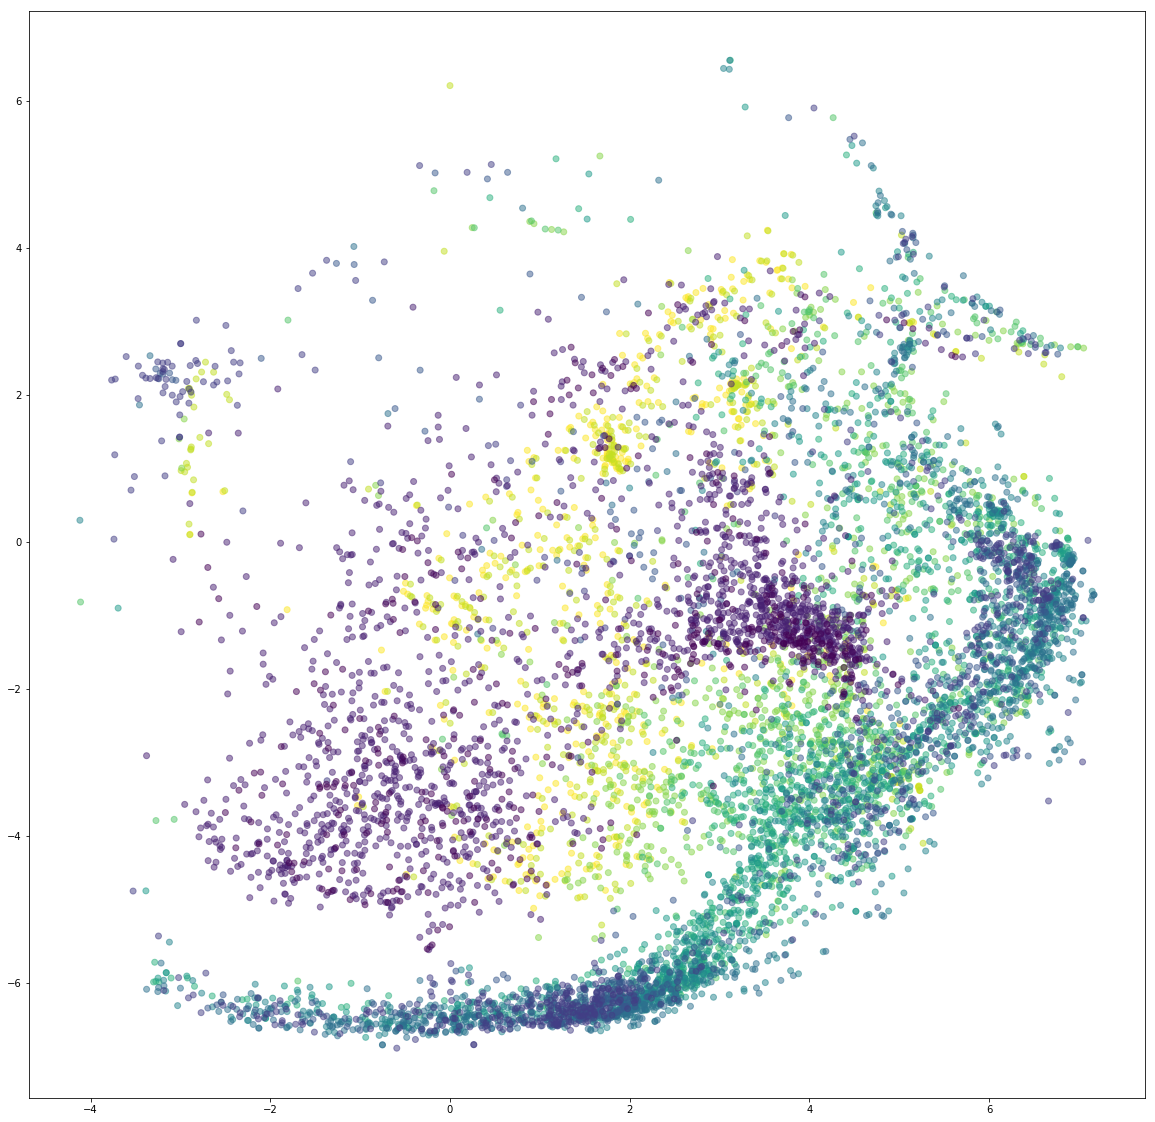
\includegraphics[scale=0.15]{P2C3}
  \label{fig:test1}
\end{minipage}
\begin{minipage}{.5\textwidth}
  \captionof{figure}{19th Century: Clementi}
  \centering
  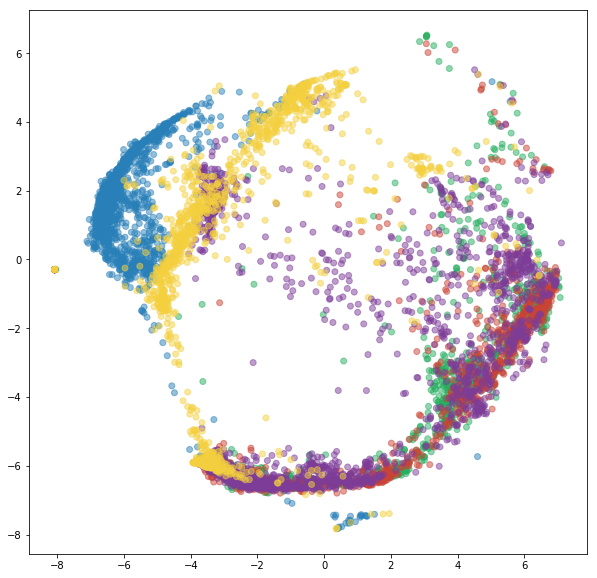
\includegraphics[scale=0.15]{P3C2}
  \label{fig:test2}
\end{minipage}
\end{figure}

Lastly, the same pattern extended until the 20th Century with composer Stravinsky. Stravinsky has a very similar pattern with the 19th Century composers. Shown below is the graph of Stravinsky.

\begin{figure}[!htb]
\caption{20th Cen: Stravinsky}
\centering
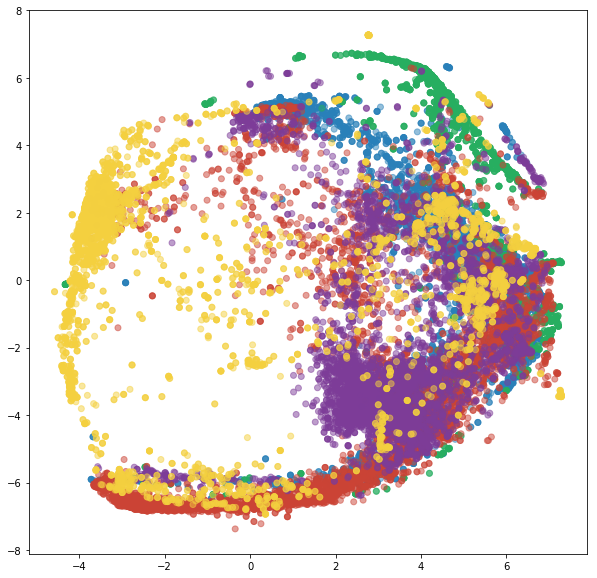
\includegraphics[scale=0.15]{P5C5}
\end{figure}

The results of the graphs may suggest that the works of the 19th and 20th Century composers are influenced by previous periods. The works of Boyce and Sammartini are the root of this specific style pattern that might be adapted to the next period. 

The researchers also noticed a pair of composers which had the most distinguishable pattern because the points are only located in the left side of the graph. 19th Century composer Gossec and 20th Century composer Antheil produced similar style pattern which may suggest that Antheil’s work is influenced by Gossec.

\begin{figure}[!htb]
\begin{minipage}{.5\textwidth}
  \captionof{figure}{19th Century: Gossec}
  \centering
  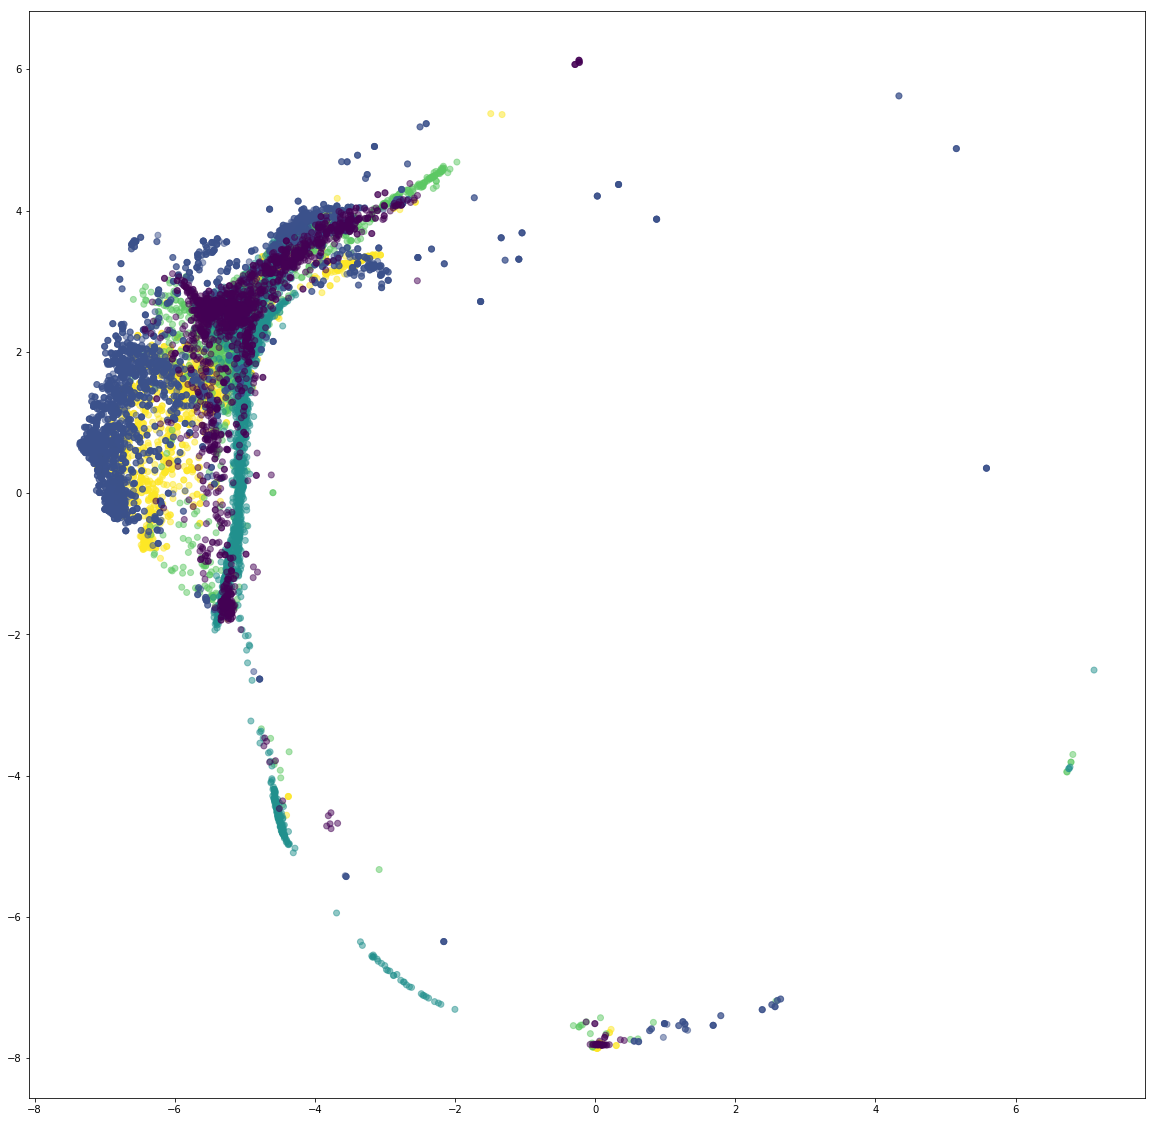
\includegraphics[scale=0.15]{P3C3}
  \label{fig:test1}
\end{minipage}
\begin{minipage}{.5\textwidth}
  \captionof{figure}{20th Cen: Antheil}
  \centering
  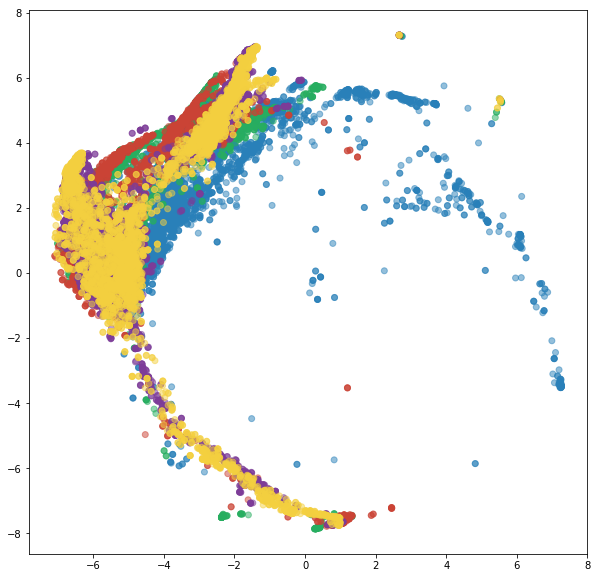
\includegraphics[scale=0.15]{P5C1}
  \label{fig:test1}
\end{minipage}
\end{figure}
\section{Quantitative Analysis}

Table 5.1 below shows the frequency count of each cluster per symphony. Each time a point is found in a cluster, the frequency count of the corresponding label is incremented. Table 5.5 shows the percentage of the same frequency distribution table of clusters per symphony. Cluster label A has the highest number of frequency with a total of 86983, followed by B with 65867, E with 65355, D with 60726, and lastly C with 51845. These cluster counts can be used to help verify the similarity of symphonies by, for example, checking the results from the above comparisons and seeing whether their cluster counts are truly similar. Since cluster counts do not incorporate the presence of time, unlike the previous comparisons, it is highly unlikely that comparisons made would be similar.and tabulated.

\begin{longtable}{|l|l|l|l|l|l|l|}
\caption{Frequency Cluster Count}
\label{my-label}\\
\hline
Row Labels & A & B & C & D & E & Grand Total \\ \hline
\endfirsthead
\endhead
%
P1C1S1 & 383 & 43 & 6 & 152 & 1 & 585 \\ \hline
P1C1S2 & 116 & 1609 & 2 & 16 & 710 & 2453 \\ \hline
P1C1S3 & 4 & 3 &  & 1 & 795 & 803 \\ \hline
P1C1S4 & 2 & 243 &  &  &  & 245 \\ \hline
P1C1S5 & 1 & 352 &  & 3 & 2 & 358 \\ \hline
P1C2S1 & 223 & 14 &  &  & 153 & 390 \\ \hline
P1C2S2 & 4 & 841 & 3 & 31 & 1 & 880 \\ \hline
P1C2S3 & 106 & 100 &  &  & 431 & 637 \\ \hline
P1C2S4 & 479 & 18 & 5 & 5 & 154 & 661 \\ \hline
P1C2S5 & 180 & 415 & 48 & 291 & 339 & 1273 \\ \hline
P1C3S1 & 1 & 41 &  &  & 596 & 638 \\ \hline
P1C3S2 & 450 & 73 & 5 & 32 & 71 & 631 \\ \hline
P1C3S3 &  & 90 &  & 1 & 227 & 318 \\ \hline
P1C3S4 & 2 & 10 &  & 387 &  & 399 \\ \hline
P1C3S5 & 276 & 2 &  & 1 & 23 & 302 \\ \hline
P1C4S1 & 58 & 99 & 20 & 82 & 22 & 281 \\ \hline
P1C4S2 & 83 & 109 &  & 2 & 783 & 977 \\ \hline
P1C4S3 & 297 & 286 & 83 & 408 & 57 & 1131 \\ \hline
P1C4S4 & 104 & 78 &  & 4 & 1344 & 1530 \\ \hline
P1C4S5 & 134 & 690 & 72 & 253 & 44 & 1193 \\ \hline
P1C5S1 & 33 & 952 & 2 & 1 & 24 & 1012 \\ \hline
P1C5S2 & 2 & 241 &  & 5 & 87 & 335 \\ \hline
P1C5S3 & 12 & 338 &  & 1 & 111 & 462 \\ \hline
P1C5S4 & 7 & 70 &  &  & 251 & 328 \\ \hline
P1C5S5 & 268 & 13 &  & 2 & 133 & 416 \\ \hline
P2C1S1 & 1369 & 643 & 228 & 414 & 121 & 2775 \\ \hline
P2C1S2 & 1055 & 827 & 77 & 398 & 180 & 2537 \\ \hline
P2C1S3 & 988 & 686 & 107 & 806 & 143 & 2730 \\ \hline
P2C1S4 & 1808 & 534 & 22 & 217 & 425 & 3006 \\ \hline
P2C1S5 & 478 & 148 & 18 & 90 & 232 & 966 \\ \hline
P2C2S1 & 86 & 91 & 40 & 40 & 191 & 448 \\ \hline
P2C2S2 & 180 & 258 & 60 & 270 & 110 & 878 \\ \hline
P2C2S3 & 336 & 1059 & 104 & 180 & 373 & 2052 \\ \hline
P2C2S4 & 353 & 287 & 39 & 32 & 454 & 1165 \\ \hline
P2C2S5 & 545 & 709 & 34 & 121 & 667 & 2076 \\ \hline
P2C3S1 & 279 & 369 & 12 & 22 & 249 & 931 \\ \hline
P2C3S2 & 72 & 206 & 2 & 8 & 804 & 1092 \\ \hline
P2C3S3 & 259 & 133 & 1 & 1 & 1218 & 1612 \\ \hline
P2C3S4 & 623 & 192 & 1 & 4 & 864 & 1684 \\ \hline
P2C3S5 & 504 & 123 & 6 & 81 & 599 & 1313 \\ \hline
P2C4S1 & 1396 & 330 & 16 & 44 & 1164 & 2950 \\ \hline
P2C4S2 & 764 & 612 & 421 & 265 & 845 & 2907 \\ \hline
P2C4S3 & 1082 & 293 & 71 & 162 & 913 & 2521 \\ \hline
P2C4S4 & 881 & 208 & 30 & 11 & 2112 & 3242 \\ \hline
P2C4S5 & 1091 & 546 & 492 & 271 & 771 & 3171 \\ \hline
P2C5S1 & 694 & 521 & 232 & 703 & 1446 & 3596 \\ \hline
P2C5S2 & 700 & 653 & 476 & 1144 & 80 & 3053 \\ \hline
P2C5S3 & 1375 & 373 & 539 & 792 & 281 & 3360 \\ \hline
P2C5S4 & 1145 & 1119 & 629 & 1408 & 26 & 4327 \\ \hline
P2C5S5 & 472 & 381 & 129 & 301 & 339 & 1622 \\ \hline
P3C1S1 & 514 & 411 & 87 & 296 & 46 & 1354 \\ \hline
P3C1S2 & 246 & 103 & 14 & 84 & 28 & 475 \\ \hline
P3C1S3 & 1460 & 258 & 65 & 112 & 498 & 2393 \\ \hline
P3C1S4 & 1032 & 102 & 15 & 29 & 933 & 2111 \\ \hline
P3C1S5 & 47 & 116 & 2 & 3 & 1109 & 1277 \\ \hline
P3C2S1 & 36 & 3 & 1653 & 237 & 2 & 1931 \\ \hline
P3C2S2 & 371 & 70 & 10 & 1 & 554 & 1006 \\ \hline
P3C2S3 & 461 & 41 & 9 &  & 531 & 1042 \\ \hline
P3C2S4 & 1048 & 102 & 80 & 199 & 574 & 2003 \\ \hline
P3C2S5 & 487 & 73 & 434 & 444 & 15 & 1453 \\ \hline
P3C3S1 & 32 &  & 1351 & 724 &  & 2107 \\ \hline
P3C3S2 & 18 &  & 1068 & 598 & 5 & 1689 \\ \hline
P3C3S3 & 173 &  & 1568 & 245 & 4 & 1990 \\ \hline
P3C3S4 & 54 & 10 & 3109 & 1114 & 4 & 4291 \\ \hline
P3C3S5 & 42 &  & 1139 & 521 &  & 1702 \\ \hline
P3C4S1 & 1028 & 139 & 53 & 378 & 462 & 2060 \\ \hline
P3C4S2 & 414 & 316 & 118 & 250 & 90 & 1188 \\ \hline
P3C4S3 & 2275 & 340 & 135 & 192 & 346 & 3288 \\ \hline
P3C4S4 & 1021 & 522 & 108 & 145 & 469 & 2265 \\ \hline
P3C4S5 & 602 & 194 & 6 & 13 & 879 & 1694 \\ \hline
P3C5S1 & 592 & 311 & 377 & 347 & 317 & 1944 \\ \hline
P3C5S2 & 1493 & 740 & 244 & 546 & 101 & 3124 \\ \hline
P3C5S3 & 1753 & 286 & 129 & 329 & 22 & 2519 \\ \hline
P3C5S4 & 713 & 126 & 14 & 28 & 938 & 1819 \\ \hline
P3C5S5 & 27 & 70 & 2 & 4 & 723 & 826 \\ \hline
P4C1S1 & 429 & 316 & 106 & 186 & 143 & 1180 \\ \hline
P4C1S2 & 820 & 2985 & 264 & 1919 & 58 & 6046 \\ \hline
P4C1S3 & 1145 & 1717 & 357 & 621 & 307 & 4147 \\ \hline
P4C1S4 & 1088 & 519 & 54 & 107 & 346 & 2114 \\ \hline
P4C1S5 & 612 & 215 & 2 & 88 & 424 & 1341 \\ \hline
P4C2S1 & 438 & 182 & 1 & 100 & 2682 & 3403 \\ \hline
P4C2S2 & 1456 & 575 & 207 & 490 & 115 & 2843 \\ \hline
P4C2S3 & 2016 & 1059 & 103 & 332 & 524 & 4034 \\ \hline
P4C2S4 & 1329 & 354 & 17 & 46 & 804 & 2550 \\ \hline
P4C2S5 & 593 & 94 &  & 15 & 848 & 1550 \\ \hline
P4C3S1 & 15 &  & 2838 & 1617 & 21 & 4491 \\ \hline
P4C3S2 & 7 &  & 2373 & 1664 & 8 & 4052 \\ \hline
P4C3S3 & 46 &  & 168 & 5139 &  & 5353 \\ \hline
P4C3S4 & 12 & 253 & 153 & 3404 & 12 & 3834 \\ \hline
P4C3S5 & 4 & 3885 &  & 62 & 99 & 4050 \\ \hline
P4C4S1 & 889 & 497 &  & 15 & 1337 & 2738 \\ \hline
P4C4S2 & 1195 & 566 & 2 & 201 & 910 & 2874 \\ \hline
P4C4S3 & 1875 & 66 & 212 & 287 & 342 & 2782 \\ \hline
P4C4S4 & 138 & 1 & 3393 & 25 &  & 3557 \\ \hline
P4C4S5 & 40 & 7 & 3044 & 60 &  & 3151 \\ \hline
P4C5S1 & 379 & 367 & 243 & 401 & 70 & 1460 \\ \hline
P4C5S2 & 673 & 250 & 204 & 327 & 140 & 1594 \\ \hline
P4C5S3 & 1866 & 331 & 157 & 398 & 408 & 3160 \\ \hline
P4C5S4 & 672 & 379 & 7 & 104 & 476 & 1638 \\ \hline
P4C5S5 & 168 & 354 & 33 & 87 & 842 & 1484 \\ \hline
P5C1S1 & 46 & 471 & 1397 & 3291 & 101 & 5306 \\ \hline
P5C1S2 & 158 & 15 & 3637 & 1511 &  & 5321 \\ \hline
P5C1S3 & 150 & 21 & 2394 & 1556 &  & 4121 \\ \hline
P5C1S4 & 472 & 11 & 3292 & 1729 &  & 5504 \\ \hline
P5C1S5 & 652 & 13 & 2826 & 2141 &  & 5632 \\ \hline
P5C2S1 & 2968 & 1071 & 756 & 822 & 75 & 5692 \\ \hline
P5C2S2 & 2594 & 683 & 1211 & 1497 & 157 & 6142 \\ \hline
P5C2S3 & 2612 & 217 & 63 & 201 & 1489 & 4582 \\ \hline
P5C2S4 & 341 & 1070 & 94 & 114 & 4240 & 5859 \\ \hline
P5C2S5 & 3811 & 854 & 690 & 526 & 385 & 3199 \\ \hline
P5C3S1 & 1194 & 1907 & 618 & 1215 & 493 & 5427 \\ \hline
P5C3S2 & 2590 & 1264 & 417 & 734 & 564 & 5569 \\ \hline
P5C3S3 & 2975 & 1009 & 212 & 786 & 419 & 5401 \\ \hline
P5C3S4 & 1460 & 534 & 20 & 730 & 1418 & 4162 \\ \hline
P5C3S5 & 2023 & 707 & 8 & 299 & 2572 & 5609 \\ \hline
P5C4S1 & 585 & 1076 & 911 & 1186 & 165 & 3923 \\ \hline
P5C4S2 & 292 & 1955 & 1144 & 1943 & 111 & 5445 \\ \hline
P5C4S3 & 624 & 2737 & 428 & 1329 & 552 & 5670 \\ \hline
P5C4S4 & 641 & 2713 & 719 & 1160 & 286 & 5519 \\ \hline
P5C4S5 & 1242 & 2513 & 299 & 561 & 424 & 5039 \\ \hline
P5C5S1 & 234 & 2447 & 6 & 360 & 3036 & 6083 \\ \hline
P5C5S2 & 58 & 3071 & 22 & 26 & 938 & 4115 \\ \hline
P5C5S3 & 2613 & 665 & 8 & 333 & 2554 & 6173 \\ \hline
P5C5S4 & 251 & 762 &  & 170 & 4067 & 5250 \\ \hline
P5C5S5 & 793 & 745 & 913 & 2509 & 777 & 5737 \\ \hline
Grand Total & 86983 & 65867 & 51845 & 60726 & 65355 & 330776 \\ \hline
\end{longtable}

\begin{longtable}{|l|l|l|l|l|l|}
\caption{Percentage Cluster Count}
\label{my-label}\\
\hline
Row Labels & A & B & C & D & E \\ \hline
\endfirsthead
\endhead
%
P1C1S1 & 65\% & 7\% & 1\% & 26\% & 0\% \\ \hline
P1C1S2 & 5\% & 66\% & 0\% & 1\% & 29\% \\ \hline
P1C1S3 & 0\% & 0\% & 0\% & 0\% & 99\% \\ \hline
P1C1S4 & 1\% & 99\% & 0\% & 0\% & 0\% \\ \hline
P1C1S5 & 0\% & 98\% & 0\% & 1\% & 1\% \\ \hline
P1C2S1 & 57\% & 4\% & 0\% & 0\% & 39\% \\ \hline
P1C2S2 & 0\% & 96\% & 0\% & 4\% & 0\% \\ \hline
P1C2S3 & 17\% & 16\% & 0\% & 0\% & 68\% \\ \hline
P1C2S4 & 72\% & 3\% & 1\% & 1\% & 23\% \\ \hline
P1C2S5 & 14\% & 33\% & 4\% & 23\% & 27\% \\ \hline
P1C3S1 & 0\% & 6\% & 0\% & 0\% & 93\% \\ \hline
P1C3S2 & 71\% & 12\% & 1\% & 5\% & 11\% \\ \hline
P1C3S3 & 0\% & 28\% & 0\% & 0\% & 71\% \\ \hline
P1C3S4 & 1\% & 3\% & 0\% & 97\% & 0\% \\ \hline
P1C3S5 & 91\% & 1\% & 0\% & 0\% & 8\% \\ \hline
P1C4S1 & 21\% & 35\% & 7\% & 29\% & 8\% \\ \hline
P1C4S2 & 8\% & 11\% & 0\% & 0\% & 80\% \\ \hline
P1C4S3 & 26\% & 25\% & 7\% & 36\% & 5\% \\ \hline
P1C4S4 & 7\% & 5\% & 0\% & 0\% & 88\% \\ \hline
P1C4S5 & 11\% & 58\% & 6\% & 21\% & 4\% \\ \hline
P1C5S1 & 3\% & 94\% & 0\% & 0\% & 2\% \\ \hline
P1C5S2 & 1\% & 72\% & 0\% & 1\% & 26\% \\ \hline
P1C5S3 & 3\% & 73\% & 0\% & 0\% & 24\% \\ \hline
P1C5S4 & 2\% & 21\% & 0\% & 0\% & 77\% \\ \hline
P1C5S5 & 64\% & 3\% & 0\% & 0\% & 32\% \\ \hline
P2C1S1 & 49\% & 23\% & 8\% & 15\% & 4\% \\ \hline
P2C1S2 & 42\% & 33\% & 3\% & 16\% & 7\% \\ \hline
P2C1S3 & 36\% & 25\% & 4\% & 30\% & 5\% \\ \hline
P2C1S4 & 60\% & 18\% & 1\% & 7\% & 14\% \\ \hline
P2C1S5 & 49\% & 15\% & 2\% & 9\% & 24\% \\ \hline
P2C2S1 & 19\% & 20\% & 9\% & 9\% & 43\% \\ \hline
P2C2S2 & 21\% & 29\% & 7\% & 31\% & 13\% \\ \hline
P2C2S3 & 16\% & 52\% & 5\% & 9\% & 18\% \\ \hline
P2C2S4 & 30\% & 25\% & 3\% & 3\% & 39\% \\ \hline
P2C2S5 & 26\% & 34\% & 2\% & 6\% & 32\% \\ \hline
P2C3S1 & 30\% & 40\% & 1\% & 2\% & 27\% \\ \hline
P2C3S2 & 7\% & 19\% & 0\% & 1\% & 74\% \\ \hline
P2C3S3 & 16\% & 8\% & 0\% & 0\% & 76\% \\ \hline
P2C3S4 & 37\% & 11\% & 0\% & 0\% & 51\% \\ \hline
P2C3S5 & 38\% & 9\% & 0\% & 6\% & 46\% \\ \hline
P2C4S1 & 47\% & 11\% & 1\% & 1\% & 39\% \\ \hline
P2C4S2 & 26\% & 21\% & 14\% & 9\% & 29\% \\ \hline
P2C4S3 & 43\% & 12\% & 3\% & 6\% & 36\% \\ \hline
P2C4S4 & 27\% & 6\% & 1\% & 0\% & 65\% \\ \hline
P2C4S5 & 34\% & 17\% & 16\% & 9\% & 24\% \\ \hline
P2C5S1 & 19\% & 14\% & 6\% & 20\% & 40\% \\ \hline
P2C5S2 & 23\% & 21\% & 16\% & 37\% & 3\% \\ \hline
P2C5S3 & 41\% & 11\% & 16\% & 24\% & 8\% \\ \hline
P2C5S4 & 26\% & 26\% & 15\% & 33\% & 1\% \\ \hline
P2C5S5 & 29\% & 23\% & 8\% & 19\% & 21\% \\ \hline
P3C1S1 & 38\% & 30\% & 6\% & 22\% & 3\% \\ \hline
P3C1S2 & 52\% & 22\% & 3\% & 18\% & 6\% \\ \hline
P3C1S3 & 61\% & 11\% & 3\% & 5\% & 21\% \\ \hline
P3C1S4 & 49\% & 5\% & 1\% & 1\% & 44\% \\ \hline
P3C1S5 & 4\% & 9\% & 0\% & 0\% & 87\% \\ \hline
P3C2S1 & 2\% & 0\% & 86\% & 12\% & 0\% \\ \hline
P3C2S2 & 37\% & 7\% & 1\% & 0\% & 55\% \\ \hline
P3C2S3 & 44\% & 4\% & 1\% & 0\% & 51\% \\ \hline
P3C2S4 & 52\% & 5\% & 4\% & 10\% & 29\% \\ \hline
P3C2S5 & 34\% & 5\% & 30\% & 31\% & 1\% \\ \hline
P3C3S1 & 2\% & 0\% & 64\% & 34\% & 0\% \\ \hline
P3C3S2 & 1\% & 0\% & 63\% & 35\% & 0\% \\ \hline
P3C3S3 & 9\% & 0\% & 79\% & 12\% & 0\% \\ \hline
P3C3S4 & 1\% & 0\% & 72\% & 26\% & 0\% \\ \hline
P3C3S5 & 2\% & 0\% & 67\% & 31\% & 0\% \\ \hline
P3C4S1 & 50\% & 7\% & 3\% & 18\% & 22\% \\ \hline
P3C4S2 & 35\% & 27\% & 10\% & 21\% & 8\% \\ \hline
P3C4S3 & 69\% & 10\% & 4\% & 6\% & 11\% \\ \hline
P3C4S4 & 45\% & 23\% & 5\% & 6\% & 21\% \\ \hline
P3C4S5 & 36\% & 11\% & 0\% & 1\% & 52\% \\ \hline
P3C5S1 & 30\% & 16\% & 19\% & 18\% & 16\% \\ \hline
P3C5S2 & 48\% & 24\% & 8\% & 17\% & 3\% \\ \hline
P3C5S3 & 70\% & 11\% & 5\% & 13\% & 1\% \\ \hline
P3C5S4 & 39\% & 7\% & 1\% & 2\% & 52\% \\ \hline
P3C5S5 & 3\% & 8\% & 0\% & 0\% & 88\% \\ \hline
P4C1S1 & 36\% & 27\% & 9\% & 16\% & 12\% \\ \hline
P4C1S2 & 14\% & 49\% & 4\% & 32\% & 1\% \\ \hline
P4C1S3 & 28\% & 41\% & 9\% & 15\% & 7\% \\ \hline
P4C1S4 & 51\% & 25\% & 3\% & 5\% & 16\% \\ \hline
P4C1S5 & 46\% & 16\% & 0\% & 7\% & 32\% \\ \hline
P4C2S1 & 13\% & 5\% & 0\% & 3\% & 79\% \\ \hline
P4C2S2 & 51\% & 20\% & 7\% & 17\% & 4\% \\ \hline
P4C2S3 & 50\% & 26\% & 3\% & 8\% & 13\% \\ \hline
P4C2S4 & 52\% & 14\% & 1\% & 2\% & 32\% \\ \hline
P4C2S5 & 38\% & 6\% & 0\% & 1\% & 55\% \\ \hline
P4C3S1 & 0\% & 0\% & 63\% & 36\% & 0\% \\ \hline
P4C3S2 & 0\% & 0\% & 59\% & 41\% & 0\% \\ \hline
P4C3S3 & 1\% & 0\% & 3\% & 96\% & 0\% \\ \hline
P4C3S4 & 0\% & 7\% & 4\% & 89\% & 0\% \\ \hline
P4C3S5 & 0\% & 96\% & 0\% & 2\% & 2\% \\ \hline
P4C4S1 & 32\% & 18\% & 0\% & 1\% & 49\% \\ \hline
P4C4S2 & 42\% & 20\% & 0\% & 7\% & 32\% \\ \hline
P4C4S3 & 67\% & 2\% & 8\% & 10\% & 12\% \\ \hline
P4C4S4 & 4\% & 0\% & 95\% & 1\% & 0\% \\ \hline
P4C4S5 & 1\% & 0\% & 97\% & 2\% & 0\% \\ \hline
P4C5S1 & 26\% & 25\% & 17\% & 27\% & 5\% \\ \hline
P4C5S2 & 42\% & 16\% & 13\% & 21\% & 9\% \\ \hline
P4C5S3 & 59\% & 10\% & 5\% & 13\% & 13\% \\ \hline
P4C5S4 & 41\% & 23\% & 0\% & 6\% & 29\% \\ \hline
P4C5S5 & 11\% & 24\% & 2\% & 6\% & 57\% \\ \hline
P5C1S1 & 1\% & 9\% & 26\% & 62\% & 2\% \\ \hline
P5C1S2 & 3\% & 0\% & 68\% & 28\% & 0\% \\ \hline
P5C1S3 & 4\% & 1\% & 58\% & 38\% & 0\% \\ \hline
P5C1S4 & 9\% & 0\% & 60\% & 31\% & 0\% \\ \hline
P5C1S5 & 12\% & 0\% & 50\% & 38\% & 0\% \\ \hline
P5C2S1 & 52\% & 19\% & 13\% & 14\% & 1\% \\ \hline
P5C2S2 & 42\% & 11\% & 20\% & 24\% & 3\% \\ \hline
P5C2S3 & 57\% & 5\% & 1\% & 4\% & 32\% \\ \hline
P5C2S4 & 6\% & 18\% & 2\% & 2\% & 72\% \\ \hline
P5C2S5 & 119\% & 27\% & 22\% & 16\% & 12\% \\ \hline
P5C3S1 & 22\% & 35\% & 11\% & 22\% & 9\% \\ \hline
P5C3S2 & 47\% & 23\% & 7\% & 13\% & 10\% \\ \hline
P5C3S3 & 55\% & 19\% & 4\% & 15\% & 8\% \\ \hline
P5C3S4 & 35\% & 13\% & 0\% & 18\% & 34\% \\ \hline
P5C3S5 & 36\% & 13\% & 0\% & 5\% & 46\% \\ \hline
P5C4S1 & 15\% & 27\% & 23\% & 30\% & 4\% \\ \hline
P5C4S2 & 5\% & 36\% & 21\% & 36\% & 2\% \\ \hline
P5C4S3 & 11\% & 48\% & 8\% & 23\% & 10\% \\ \hline
P5C4S4 & 12\% & 49\% & 13\% & 21\% & 5\% \\ \hline
P5C4S5 & 25\% & 50\% & 6\% & 11\% & 8\% \\ \hline
P5C5S1 & 4\% & 40\% & 0\% & 6\% & 50\% \\ \hline
P5C5S2 & 1\% & 75\% & 1\% & 1\% & 23\% \\ \hline
P5C5S3 & 42\% & 11\% & 0\% & 5\% & 41\% \\ \hline
P5C5S4 & 5\% & 15\% & 0\% & 3\% & 77\% \\ \hline
P5C5S5 & 14\% & 13\% & 16\% & 44\% & 14\% \\ \hline
\end{longtable}

Listed below in table 5.3 are the results of using Manhattan distance for pairwise comparison of symphonies with respect to the time dimension of each symphonies. Each point in time of the t-SNE result for a symphony is matched with a point of another symphony and the distance between these two points is computed. The process is simply repeated until the end of either symphony is reached. Truncation is thus performed on the longer string to match the lengths of the two symphonies being compared. The resulting collection of distances are thus summed 

The results show that Bach’s sinfonia no. 7 and sinfonia no. 4 are the most similar among the entire list of symphonies, followed by Gabrieli’s canzon noni toni a 12-correggio with Viadana’s sinfonia la bolognese, and so on. Contrary to expectation that symphonies from the same composer would be more similar compared to those of other composers, a lot of entries in the top 30 have symphonies that come from different composers. Interestingly, a lot of entries in the top 30 also come from Bach’s sinfonia no. 7, which could very well indicate that its points may be well scattered throughout the map when plotted or the points could be positioned near the center of the map. Verifying this, we look at Bach’s graph in Figure 5.6 and the green points, which represent Bach’s sinfonia no. 7 are somewhat located near the middle of the graph. They are not, however, scattered throughout the map. Viadana’s Sinfonia la Bergamasca is the second most number of matches in the top 30 and based on its graph in Figure 5.10, it can be seen that this symphony is somewhat scattered but the main bulk of its points are still near the middle. Seeing this result may well indicate that symphonies located near the middle when graphed may have a stronger tendency to have higher matches with more symphonies when comparing through distances of points via time. To furr verify this method of comparison between symphonies, we shall compare these results with the results of other metrics later on. The results of this metric together with other succeeding partial results below can be further viewed in their respective spreadsheet files as the results of these pairwise comparisons have a total number of 125x125 rows.

\begin{longtable}{|l|l|l|}
\caption{Manhattan Distance Top Results: Full Length Summed}
\label{my-label}\\
\hline
Symphony A & Symphony B & Distance Sum \\ \hline
\endfirsthead
\endhead
%
P1C1S4 & P1C1S5 & 269.9242 \\ \hline
P1C3S3 & P1C5S4 & 598.8077 \\ \hline
P1C1S4 & P1C5S3 & 776.0105 \\ \hline
P1C1S4 & P1C3S3 & 787.6107 \\ \hline
P1C1S4 & P1C5S4 & 807.6517 \\ \hline
P1C4S1 & P1C4S3 & 947.415 \\ \hline
P1C3S3 & P1C5S3 & 967.2533 \\ \hline
P1C1S5 & P1C5S3 & 970.1439 \\ \hline
P1C4S1 & P1C4S5 & 993.4798 \\ \hline
P1C1S4 & P5C5S2 & 999.3968 \\ \hline
P1C4S1 & P4C1S2A & 1010.578 \\ \hline
P1C1S4 & P1C2S2 & 1017.719 \\ \hline
P1C1S4 & P1C5S2 & 1027.048 \\ \hline
P1C4S1 & P5C3S3A & 1034.093 \\ \hline
P1C4S1 & P2C5S2A & 1045.884 \\ \hline
P1C4S1 & P2C2S2A & 1059.302 \\ \hline
P1C4S1 & P2C5S4A & 1074.551 \\ \hline
P1C4S1 & P4C1S3A & 1104.918 \\ \hline
P1C4S1 & P3C5S3 & 1117.526 \\ \hline
P1C4S1 & P4C2S3A & 1130.082 \\ \hline
P1C4S1 & P3C1S1 & 1153.61 \\ \hline
P1C4S1 & P2C1S3 & 1156.801 \\ \hline
P1C4S1 & P3C1S2 & 1158.137 \\ \hline
P1C1S4 & P1C2S5 & 1167.234 \\ \hline
P1C4S1 & P4C1S4 & 1181.949 \\ \hline
P1C4S1 & P2C1S2 & 1186.405 \\ \hline
P1C4S1 & P3C5S2 & 1198.531 \\ \hline
P1C1S4 & P1C3S1 & 1222.162 \\ \hline
P1C4S1 & P2C3S1A & 1225.814 \\ \hline
P1C4S1 & P2C1S1 & 1234.873 \\ \hline
P1C4S1 & P4C1S1A & 1238.681 \\ \hline
\end{longtable}

Table 5.4 below shows the Manhattan distance comparison of symphonies, but this time, through the transitions only. Interestingly, a lot of the rankings of the results matched that of the earlier comparisons like for example, a lot of the top 30 results here still showed Bach’s sinfonia no. 7.

\begin{longtable}{|l|l|l|}
\caption{Manhattan Distance Result: Transitions Summed}
\label{my-label}\\
\hline
Symphony A & Symphony B & Distance Sum \\ \hline
\endfirsthead
%
\endhead
%
P2C1S3 & P1C1S4 & 6.342487 \\ \hline
P2C5S3A & P1C1S4 & 7.09482 \\ \hline
P3C1S3 & P1C1S4 & 7.191891 \\ \hline
P2C4S2A & P1C1S4 & 7.276127 \\ \hline
P1C1S4 & P1C1S5 & 7.354168 \\ \hline
P4C2S1A & P1C1S4 & 7.489208 \\ \hline
P1C2S5 & P1C1S4 & 7.49975 \\ \hline
P2C3S1A & P1C1S4 & 7.522169 \\ \hline
P1C1S5 & P1C1S4 & 7.667543 \\ \hline
P1C1S4 & P1C5S5 & 7.682119 \\ \hline
P1C1S4 & P2C3S2A & 7.769781 \\ \hline
P2C3S2A & P1C1S4 & 7.805628 \\ \hline
P2C1S4 & P1C1S4 & 7.806015 \\ \hline
P2C2S5A & P1C1S4 & 7.961077 \\ \hline
P2C3S3A & P1C1S4 & 7.981119 \\ \hline
P5C2S3 & P1C1S4 & 8.046022 \\ \hline
P1C2S3 & P1C2S3 & 8.079905 \\ \hline
P4C1S1A & P1C1S4 & 8.13656 \\ \hline
P4C1S5A & P1C1S4 & 8.149289 \\ \hline
P2C4S1A & P1C1S4 & 8.167969 \\ \hline
P2C2S1 & P1C1S4 & 8.23078 \\ \hline
P4C5S4 & P1C1S4 & 8.290154 \\ \hline
P2C5S1A & P1C1S4 & 8.318904 \\ \hline
P5C5S4 & P1C1S4 & 8.383004 \\ \hline
P1C1S4 & P2C5S1A & 8.563907 \\ \hline
P1C1S4 & P1C1S2 & 8.621842 \\ \hline
P1C1S4 & P5C3S1A & 8.723814 \\ \hline
P1C4S5 & P1C1S4 & 8.732073 \\ \hline
P4C4S2 & P1C1S4 & 8.783347 \\ \hline
P1C1S4 & P3C1S5 & 8.82796 \\ \hline
\end{longtable}

If we take the the top results from the Manhattan distance above, with Bach’s sinfonia no. 7 (P1C1S4) and sinfonia no. 4 (P1C1S5) being the top for Manhattan distance comparison, we can see below in Table 5.4 that indeed their cluster couts are somewhat similar with the majority of the points being in cluster B. Sinfonia no. 7 has 99\% of points in B while sinfonia no. 4 has 98\% of points in B.  The second closest with the Manhattan result, Gabrieli’s canzon noni toni a 12-correggio (P1C3S3) and Viadana’s sinfonia la bolognese (P1C5S4), again show the same result with their cluster counts being very similar in that both of them had near 75\% of points in cluster E and nea 25\% in cluster B.

Bach’s sinfonia no. 7 (P1C1S4) which produced a lot of high matches with other symphonies is also coincidentally the shortest symphony among the dataset and this may indicate that truncation indeed is not a reliable method of matching the lengths of the symphonies for comparison or it could also mean that sinfonia no. 7 simply has a lot in common with most symphonies. In order to further verify this, we repeat the Manhattan distance comparison, but this time, by taking the average of the distances of all the points that were compared instead of simply adding them all up. Table 5.5 below shows the top 30 results. Bach’s sinfonia no. 7 can still be seen in some entries but the entries this time around have more variance in them unlike the total distance from before.

\begin{longtable}{|l|l|l|}
\caption{Manhattan Distance Result: Distances Mean}
\label{my-label}\\
\hline
Symphony A & Symphony B & Distance Mean \\ \hline
\endfirsthead
%
\endhead
%
P1C1S4 & P1C1S5 & 1.106247 \\ \hline
P1C3S3 & P1C5S4 & 1.888983 \\ \hline
P3C3S2 & P3C3S5 & 2.709862 \\ \hline
P1C1S5 & P1C5S3 & 2.71749 \\ \hline
P4C4S4 & P4C4S5 & 2.783062 \\ \hline
P3C2S1 & P3C3S1 & 2.885411 \\ \hline
P3C3S1 & P3C3S2 & 2.894063 \\ \hline
P1C3S3 & P1C5S3 & 3.051272 \\ \hline
P3C2S1 & P3C3S4 & 3.158728 \\ \hline
P1C1S4 & P1C5S3 & 3.180371 \\ \hline
P3C3S1 & P3C3S3 & 3.197033 \\ \hline
P3C3S2 & P3C3S3 & 3.213563 \\ \hline
P1C1S4 & P1C3S3 & 3.227913 \\ \hline
P3C3S1 & P3C3S4 & 3.303385 \\ \hline
P1C1S4 & P1C5S4 & 3.310048 \\ \hline
P1C1S1 & P3C5S3 & 3.356575 \\ \hline
P1C4S1 & P1C4S3 & 3.383625 \\ \hline
P3C2S1 & P3C3S2 & 3.384755 \\ \hline
P3C1S4 & P4C2S1A & 3.422252 \\ \hline
P1C1S1 & P1C3S2 & 3.433787 \\ \hline
P2C4S4A & P4C2S1A & 3.438686 \\ \hline
P1C1S1 & P3C1S1 & 3.472338 \\ \hline
P3C1S4 & P3C5S4 & 3.541771 \\ \hline
P3C4S5 & P4C2S1A & 3.548003 \\ \hline
P1C4S1 & P1C4S5 & 3.548142 \\ \hline
P1C5S1 & P4C3S5 & 3.583475 \\ \hline
P3C5S4 & P4C2S1A & 3.58519 \\ \hline
P3C2S1 & P3C3S3 & 3.594948 \\ \hline
P1C4S1 & P4C1S2A & 3.609206 \\ \hline
P2C4S4A & P3C1S4 & 3.637364 \\ \hline
P1C1S1 & P4C5S2 & 3.6608 \\ \hline
\end{longtable}

Table 5.6 below shows the top results when longest common subsequence (LCS) is used and the symphony points were truncated to match each pair of symphonies. Table 5.7 shows the top results when LCS was used and no truncation was done. When truncation was done, a lot of top results became perfect matches as seen below and due to this, the results are deemed bad and inapproriate for comparison. The untruncated version shows better results with the top match being 61\%. Table 5.8, on the other hand, shows LCS results using the transitions only. This resulted in overall lower percentage matches but may still be a good metric and shall be evaluated further later on.

\begin{longtable}{|l|l|l|}
\caption{LCS Truncated Result}
\label{my-label}\\
\hline
Symphony A & Symphony B & Percent Match \\ \hline
\endfirsthead
%
\endhead
%
P1C1S3 & P1C4S4 & 100\% \\ \hline
P1C1S3 & P2C3S4A & 100\% \\ \hline
P1C1S3 & P2C4S1A & 100\% \\ \hline
P1C1S3 & P2C4S2A & 100\% \\ \hline
P1C1S3 & P2C4S3A & 100\% \\ \hline
P1C1S3 & P2C4S4A & 100\% \\ \hline
P1C1S3 & P2C5S1A & 100\% \\ \hline
P1C1S3 & P3C1S4 & 100\% \\ \hline
P1C1S3 & P3C1S5 & 100\% \\ \hline
P1C1S3 & P4C2S1A & 100\% \\ \hline
P1C1S3 & P4C4S1 & 100\% \\ \hline
P1C1S3 & P4C4S2 & 100\% \\ \hline
P1C1S3 & P5C2S3 & 100\% \\ \hline
P1C1S3 & P5C2S4A & 100\% \\ \hline
P1C1S3 & P5C3S4 & 100\% \\ \hline
P1C1S3 & P5C3S5A & 100\% \\ \hline
P1C1S3 & P5C5S1A & 100\% \\ \hline
P1C1S3 & P5C5S3 & 100\% \\ \hline
P1C1S3 & P5C5S4 & 100\% \\ \hline
P1C1S4 & P1C1S2 & 100\% \\ \hline
P1C1S4 & P1C2S5 & 100\% \\ \hline
P1C1S4 & P1C4S3 & 100\% \\ \hline
P1C1S4 & P1C4S5 & 100\% \\ \hline
P1C1S4 & P1C5S1 & 100\% \\ \hline
P1C1S4 & P2C1S1 & 100\% \\ \hline
P1C1S4 & P2C1S2 & 100\% \\ \hline
P1C1S4 & P2C1S3 & 100\% \\ \hline
P1C1S4 & P2C1S4 & 100\% \\ \hline
P1C1S4 & P2C2S2A & 100\% \\ \hline
P1C1S4 & P2C2S3A & 100\% \\ \hline
\end{longtable}

\begin{longtable}{|l|l|l|}
\caption{LCS Full Length Result}
\label{my-label}\\
\hline
Symphony A & Symphony B & Percent Match \\ \hline
\endfirsthead
%
\endhead
%
P2C4S4A & P2C4S4A & 61\% \\ \hline
P2C5S2A & P2C5S2A & 58\% \\ \hline
P2C5S4A & P5C2S2A & 56\% \\ \hline
P2C4S1A & P2C4S1A & 56\% \\ \hline
P2C4S4A & P5C3S5A & 55\% \\ \hline
P2C5S4A & P5C4S2A & 54\% \\ \hline
P2C4S4A & P5C5S3 & 53\% \\ \hline
P2C5S4A & P5C4S3A & 53\% \\ \hline
P2C5S4A & P5C5S5A & 51\% \\ \hline
P2C5S4A & P5C2S1A & 51\% \\ \hline
P2C5S4A & P5C4S4A & 49\% \\ \hline
P2C5S3A & P5C2S2A & 49\% \\ \hline
P2C4S1A & P5C5S3 & 49\% \\ \hline
P2C5S1A & P5C3S5A & 49\% \\ \hline
P2C5S4A & P5C3S1A & 49\% \\ \hline
P2C4S4A & P5C2S4A & 48\% \\ \hline
P2C5S4A & P5C3S2A & 48\% \\ \hline
P2C4S4A & P5C5S4 & 47\% \\ \hline
P2C1S4 & P5C5S3 & 47\% \\ \hline
P2C4S4A & P5C5S1A & 47\% \\ \hline
P2C5S4A & P5C3S3A & 47\% \\ \hline
P2C4S4A & P4C2S1A & 46\% \\ \hline
P2C1S4 & P5C3S3A & 46\% \\ \hline
P2C5S4A & P5C4S5A & 46\% \\ \hline
P2C1S4 & P5C2S5A & 46\% \\ \hline
P2C5S3A & P5C2S1A & 46\% \\ \hline
P2C1S4 & P5C3S2A & 45\% \\ \hline
P2C1S4 & P5C2S1A & 45\% \\ \hline
P2C5S4A & P5C4S1A & 45\% \\ \hline
P2C5S2A & P5C2S2A & 45\% \\ \hline
\end{longtable}

\begin{longtable}{|l|l|l|}
\caption{LCS  Transitions Result}
\label{my-label}\\
\hline
Symphony A & Symphony B & Percentage Match \\ \hline
\endfirsthead
%
\endhead
%
P2C5S4A & P5C2S2A & 42\% \\ \hline
P5C5S5A & P5C2S2A & 41\% \\ \hline
P5C4S3A & P5C5S5A & 41\% \\ \hline
P5C5S5A & P5C4S3A & 41\% \\ \hline
P5C2S1A & P5C2S2A & 41\% \\ \hline
P2C5S4A & P5C4S3A & 41\% \\ \hline
P5C4S2A & P5C5S5A & 40\% \\ \hline
P5C2S2A & P5C4S2A & 40\% \\ \hline
P5C2S2A & P5C4S3A & 40\% \\ \hline
P5C4S3A & P5C4S4A & 40\% \\ \hline
P2C5S4A & P5C4S2A & 40\% \\ \hline
P5C3S1A & P5C4S3A & 39\% \\ \hline
P5C2S2A & P5C3S2A & 39\% \\ \hline
P5C4S2A & P5C4S4A & 38\% \\ \hline
P5C4S3A & P5C5S1A & 38\% \\ \hline
P2C5S4A & P5C5S5A & 38\% \\ \hline
P5C3S2A & P5C4S3A & 37\% \\ \hline
P5C3S5A & P5C5S1A & 37\% \\ \hline
P2C5S4A & P5C2S1A & 37\% \\ \hline
P5C4S3A & P5C4S5A & 37\% \\ \hline
P5C1S4A & P5C1S5A & 37\% \\ \hline
P2C5S4A & P5C4S4A & 36\% \\ \hline
P5C3S5A & P5C5S3 & 36\% \\ \hline
P5C2S2A & P5C3S1A & 36\% \\ \hline
P5C4S4A & P5C5S5A & 36\% \\ \hline
P5C1S5A & P5C2S2A & 36\% \\ \hline
P5C2S2A & P5C4S4A & 36\% \\ \hline
P2C5S4A & P5C3S2A & 36\% \\ \hline
P2C5S4A & P5C3S1A & 35\% \\ \hline
P5C2S1A & P5C4S3A & 35\% \\ \hline
\end{longtable}

Table 5.9 below shows the top results for sequence matcher as was discussed in Chapter 4.

\begin{longtable}{|l|l|l|}
\caption{Sequence Match Result}
\label{my-label}\\
\hline
Symphony A & Symphony B & Percentage Match \\ \hline
\endfirsthead
%
\endhead
%
P1C3S1 & P1C5S2 & 83\% \\ \hline
P1C5S5 & P3C2S3 & 76\% \\ \hline
P1C5S2 & P1C5S4 & 74\% \\ \hline
P1C2S3 & P1C2S4 & 72\% \\ \hline
P4C3S2 & P3C2S1 & 69\% \\ \hline
P1C4S2 & P1C4S4 & 68\% \\ \hline
P1C2S4 & P3C2S2 & 68\% \\ \hline
P1C3S1 & P1C3S3 & 67\% \\ \hline
P3C2S2 & P1C2S4 & 67\% \\ \hline
P1C3S1 & P1C5S4 & 64\% \\ \hline
P3C3S2 & P3C2S1 & 63\% \\ \hline
P1C5S3 & P1C5S4 & 63\% \\ \hline
P1C5S5 & P3C2S2 & 62\% \\ \hline
P1C3S5 & P1C5S5 & 61\% \\ \hline
P1C2S1 & P1C5S5 & 61\% \\ \hline
P1C2S4 & P1C5S5 & 60\% \\ \hline
P1C2S4 & P1C2S1 & 60\% \\ \hline
P1C3S1 & P1C5S3 & 59\% \\ \hline
P1C2S1 & P1C2S4 & 59\% \\ \hline
P3C1S5 & P3C2S2 & 59\% \\ \hline
P3C4S5 & P1C4S2 & 59\% \\ \hline
P1C5S1 & P3C5S5 & 58\% \\ \hline
P3C2S3 & P1C4S2 & 58\% \\ \hline
P3C4S5 & P1C4S4 & 58\% \\ \hline
P3C2S3 & P3C5S5 & 57\% \\ \hline
P3C2S2 & P3C1S5 & 57\% \\ \hline
P3C3S5 & P3C2S1 & 57\% \\ \hline
P3C2S2 & P1C5S5 & 57\% \\ \hline
P1C5S2 & P1C5S3 & 57\% \\ \hline
P4C3S3 & P3C2S1 & 57\% \\ \hline
\end{longtable}

Levenshtein distance was applied to the cluster trajectories of the each symphony. Given the trajectory of the symphony, which is represented by letters from A to E, the researchers compared all of the symphonies and tabulated their respective Levenshtein distances. The same is done to the compressed version of these trajectories.  Table 5.10 shows the results of Levenshtein using the full length data while 5.11 shows the transitions results.

\begin{longtable}{|l|l|l|}
\caption{Levenshtein Result - Full Length}
\label{my-label}\\
\hline
Symphony A & Symphony B & Distance \\ \hline
\endfirsthead
%
\endhead
%
P1C1S4 & P1C5S2 & 95 \\ \hline
P1C3S3 & P1C5S4 & 102 \\ \hline
P1C1S3 & P3C5S5 & 107 \\ \hline
P1C1S5 & P1C5S2 & 114 \\ \hline
P1C1S4 & P1C1S5 & 115 \\ \hline
P1C1S5 & P1C5S3 & 125 \\ \hline
P1C2S1 & P1C3S5 & 147 \\ \hline
P1C3S5 & P1C5S5 & 155 \\ \hline
P1C2S2 & P1C5S1 & 167 \\ \hline
P1C1S4 & P1C4S1 & 180 \\ \hline
P1C2S1 & P1C5S5 & 184 \\ \hline
P1C3S3 & P1C5S2 & 188 \\ \hline
P1C1S3 & P1C4S2 & 194 \\ \hline
P1C5S2 & P1C5S4 & 202 \\ \hline
P1C1S3 & P1C3S1 & 205 \\ \hline
P1C5S2 & P1C5S3 & 205 \\ \hline
P1C3S1 & P3C5S5 & 207 \\ \hline
P1C2S3 & P1C3S1 & 217 \\ \hline
P1C1S4 & P1C5S3 & 219 \\ \hline
P1C3S5 & P3C1S2 & 223 \\ \hline
P1C4S1 & P1C5S2 & 226 \\ \hline
P1C1S4 & P1C3S3 & 228 \\ \hline
P1C2S1 & P1C5S4 & 234 \\ \hline
P1C3S3 & P2C2S1 & 234 \\ \hline
P1C3S5 & P1C4S1 & 238 \\ \hline
P1C2S4 & P1C3S2 & 240 \\ \hline
P1C3S3 & P1C4S1 & 242 \\ \hline
P1C4S2 & P3C5S5 & 244 \\ \hline
P1C5S4 & P2C2S1 & 249 \\ \hline
P1C2S1 & P1C3S3 & 252 \\ \hline
\end{longtable}

\begin{longtable}{|l|l|l|}
\caption{Levenshtein Transitions Result}
\label{my-label}\\
\hline
Symphony A & Symphony B & Distance \\ \hline
\endfirsthead
%
\endhead
%
P1C1S3 & P1C1S5 & 6 \\ \hline
P1C1S5 & P1C3S4 & 6 \\ \hline
P1C1S3 & P1C1S4 & 8 \\ \hline
P1C1S4 & P1C1S5 & 8 \\ \hline
P1C3S1 & P1C5S4 & 8 \\ \hline
P1C1S3 & P1C3S4 & 11 \\ \hline
P1C1S4 & P1C3S4 & 12 \\ \hline
P1C3S1 & P1C5S2 & 12 \\ \hline
P1C3S5 & P1C5S3 & 14 \\ \hline
P1C1S5 & P1C5S3 & 15 \\ \hline
P1C2S1 & P1C5S5 & 15 \\ \hline
P1C3S4 & P1C5S3 & 15 \\ \hline
P1C5S2 & P1C5S4 & 15 \\ \hline
P1C1S3 & P1C5S3 & 16 \\ \hline
P1C1S3 & P1C3S5 & 17 \\ \hline
P1C1S4 & P1C5S3 & 20 \\ \hline
P1C3S1 & P1C5S3 & 21 \\ \hline
P1C1S5 & P1C3S5 & 22 \\ \hline
P1C2S1 & P1C2S3 & 22 \\ \hline
P1C5S3 & P1C5S4 & 22 \\ \hline
P1C1S4 & P1C3S5 & 23 \\ \hline
P1C3S4 & P1C3S5 & 24 \\ \hline
P1C2S1 & P3C2S3 & 25 \\ \hline
P1C2S3 & P3C2S3 & 25 \\ \hline
P1C3S5 & P1C5S4 & 25 \\ \hline
P1C2S2 & P1C5S2 & 27 \\ \hline
P1C2S3 & P1C2S4 & 27 \\ \hline
P1C5S5 & P3C2S3 & 27 \\ \hline
P1C3S1 & P1C3S5 & 28 \\ \hline
P1C5S2 & P1C5S5 & 28 \\ \hline
\end{longtable}

In order to verify which metric was the best, we compare the top 30 most similar pairs of symphonies generated by each metric and find out which two metrics had the most matches. Note also that we chose to include different implementations for each algorithm like the mean procedure of Manhattan distance over the summation procedure. Based on Table 5.12 below, mean and summation procedure of Manhattan distance would produce non-similar results since only 10 out of 30 matched. 

Among the different metrics, Levenshtein and sequence match matched best with 8 out of 30 matches, although the score is still low. Manhattan distance and Edit Distance had the most number of entries in the top 10, with Manhattan distance sum having 5 entries while the mean version having 3. Edit Distance has a total of 3 for the full length and 3 for the transitions. LCS had the worst performance with all its entries below the top 10 and sequence match performed decent with half of its entries above the top 10 and the rest below.

There resulted a total of 12 entries for the non-transitions and 8 for transitions which means that testing only the transitions for comparison is not enough to find similarities as its results are more inconsistent compared to that of the original length.

\begin{longtable}[c]{|l|l|l|}
\caption{Metric Evaluation from Pairwise Symphonies}
\label{my-label}\\
\hline
Metric 1 & Metric 2 & Matches \\ \hline
\endfirsthead
%
\endhead
%
Manhattan Distance Mean & Manhattan Distance Sum & 10 \\ \hline
Manhattan Distance Mean & LCS Truncated & 1 \\ \hline
Manhattan Distance Mean & Sequence Match & 1 \\ \hline
Manhattan Distance Sum & LCS Truncated & 0 \\ \hline
Manhattan Distance Sum & Sequence Match & 0 \\ \hline
LCS Truncated & Sequence Match & 0 \\ \hline
Manhattan Distance Transition Sum & Manhattan Distance Mean & 2 \\ \hline
Manhattan Distance Transition Sum & Manhattan Distance Sum & 3 \\ \hline
Manhattan Distance Transition Sum & LCS Truncated & 0 \\ \hline
Manhattan Distance Transition Sum & Sequence Match & 1 \\ \hline
Edit Distance Full & Manhattan Distance Mean & 5 \\ \hline
Edit Distance Full & Manhattan Distance Sum & 6 \\ \hline
Edit Distance Full & LCS Truncated & 0 \\ \hline
Edit Distance Full & Sequence Match & 4 \\ \hline
Edit Distance Full & Manhattan Distance Transition Sum & 2 \\ \hline
Edit Distance Transitions & Manhattan Distance Mean & 3 \\ \hline
Edit Distance Transitions & Manhattan Distance Sum & 3 \\ \hline
Edit Distance Transitions & LCS Truncated & 0 \\ \hline
Edit Distance Transitions & Sequence Match & 8 \\ \hline
Edit Distance Transitions & Manhattan Distance Transition Sum & 2 \\ \hline
Edit Distance Transitions & Edit Distance Full & 5 \\ \hline
\end{longtable}

In order to evaluate which composers had a wider impact to other symphonies, we tabulate the average distances or percentage per composer per era to see which composer had the least distance or the highest percentage. If different metrics produce similar results, then we can say that those metrics produced good results. Table 5.13 shows the average number of edits per composer, under each era. The table shows that Gabrieli (P1C3) has the lowest average Levenshtein distance from all of the composers across all eras while Rachmaninoff (P5C2) has the largest. It can be seen that composers from the 20th Century era (P5) returned the largest results, this could be due to the fact that the symphonies are longer than the other symphonies, which results to them having a longer trajectory string. In order to address the issue, the researchers have normalized the Levenshtein distances by dividing the results by the length of the longer trajectory string.

\begin{longtable}{|l|l|l|l|l|l|}
\caption{Average Levenshtein Distance per Composer}
\label{my-label}\\
\hline
Row & Baroque & Classical & 19th Century & Romantic & 20th Century \\ \hline
\endfirsthead
%
\endhead
%
C1 & 1191.4 & 1120.7 & 1420.6 & 3097.2 & 2447.4 \\ \hline
C2 & 724.5 & 1204 & 1309.1 & 2232.6 & 4005.6 \\ \hline
C3 & 468.3 & 815.3 & 1424.7 & 3308.7 & 3380.3 \\ \hline
C4 & 1018 & 1755.8 & 1639.6 & 2451 & 3133.3 \\ \hline
C5 & 503 & 2378.3 & 1852.2 & 1559.4 & 3863 \\ \hline
\end{longtable}

\begin{longtable}{|l|l|l|l|l|l|}
\caption{My caption}
\label{my-label}\\
\hline
Row & Baroque & Classical & 19th Century & Romantic & 20th Century \\ \hline
\endfirsthead
%
\endhead
%
C1 & 0.854 & 0.439 & 0.693 & 0.705 & 0.436 \\ \hline
C2 & 0.743 & 0.681 & 0.721 & 0.701 & 0.66-1 \\ \hline
C3 & 0.857 & 0.538 & 0.442 & 0.7101 & 0.611 \\ \hline
C4 & 0.781 & 0.569 & 0.635 & 0.755 & 0.569 \\ \hline
C5 & 0.736 & 0.63 & 0.717 & 0.7 & 0.649 \\ \hline
\end{longtable}

The researchers experimented on compressing the trajectory string, only taking into consideration the different transitions from letter to letter, ignoring the number of times the letter was repeated. This compressed trajectory string will now be compared using Levenshtein distance. Table 5.15 shows the average Levenshtein distances per composer using the compressed trajectory string. Viadana (P1C5) has the lowest average Levenshtein distance.

\begin{longtable}{|l|l|l|l|l|l|}
\caption{Average Levenshtein Distance (Compressed) per Composer}
\label{my-label}\\
\hline
Row & Baroque & Classical & 19th Century & Romantic & 20th Century \\ \hline
\endfirsthead
%
\endhead
%
C1 & 160.7 & 422.6 & 229.5 & 852.3 & 702.3 \\ \hline
C2 & 272.1 & 623 & 199.1 & 674.4 & 1736.7 \\ \hline
C3 & 111.2 & 191.7 & 509.7 & 260.5 & 1547.7 \\ \hline
C4 & 228.3 & 795.6 & 290.1 & 428.1 & 1583.2 \\ \hline
C5 & 40.1 & 1448.3 & 403.2 & 302.1 & 1581.6 \\ \hline
\end{longtable}

The compressed trajectory strings also underwent normalized Levenshtein distance and results are shown in Table 5.16. Antheil (P5C1) is shown to have the smallest average Levenshtein distance. It also can be noted that having a low Levenshtein distance does not not guarantee having a low normalized Levenshtein distance. In this case, 

\begin{longtable}{|l|l|l|l|l|l|}
\caption{Average Normalized Levenshtein Distance (Compressed) per Composer}
\label{my-label}\\
\hline
Row & Baroque & Classical & 19th Century & Romantic & 20th Century \\ \hline
\endfirsthead
%
\endhead
%
C1 & 0.873 & 0.58 & 0.624 & 0.593 & 0.319 \\ \hline
C2 & 0.697 & 0.641 & 0.693 & 0.54 & 0.621 \\ \hline
C3 & 0.807 & 0.382 & 0.579 & 0.626 & 0.532 \\ \hline
C4 & 0.64 & 0.485 & 0.54 & 0.722 & 0.492 \\ \hline
C5 & 0.559 & 0.565 & 0.676 & 0.584 & 0.544 \\ \hline
\end{longtable}

Similarly, the result from Manhattan distance was tabulated to show the average distances of each composer per era as seen in Table 5.17. The result shows that Gabrieli of Baroque era (P1C3) had the smallest distance value using the Manhattan while Schubert of Romantic era (P4C3) had the largest. This means that Gabrieli had symphonies that are closer to more symphonies than by other composers while Schubert had symphonies that are more dissimilar to other symphonies. Baroque era, in general, also had overall smaller distances compared to other eras while Romantic era had the largest.

\begin{longtable}{|l|l|l|l|l|l|}
\caption{Average Manhattan Distance per Composer}
\label{my-label}\\
\hline
Row & Baroque & Classical & 19th Century & Romantic & 20th Century \\ \hline
\endfirsthead
%
\endhead
%
C1 & 8166.221 & 15215.32 & 10140.51 & 15769.45 & 23068.61 \\ \hline
C2 & 6089.764 & 8331.856 & 13083.8 & 14746.23 & 19661.5 \\ \hline
C3 & 4140.392 & 9954.428 & 17667.8 & 27076.32 & 18392.58 \\ \hline
C4 & 7199.323 & 16218.67 & 11979.14 & 19391.64 & 20215.49 \\ \hline
C5 & 4918.109 & 17404.75 & 12183.51 & 13561.83 & 22579.82 \\ \hline
\end{longtable}

Using the normalized Manhattan distance results with the same procedure as above, it can be seen in Table 5.18 that this time, Viadana of Baroque era (P1C5) had the smallest distance, although Gabrieli, the smallest distance from the non-normalized manhattan distance result, still had a very small distance compared to most composers. This time, however, Antheil of 20th Century had the largest distance instead of Schubert

\begin{longtable}{|l|l|l|l|l|l|}
\caption{Average Normalized Manhattan Distance per Composer}
\label{my-label}\\
\hline
Row & Baroque & Classical & 19th Century & Romantic & 20th Century \\ \hline
\endfirsthead
%
\endhead
%
C1 & 491.3077674 & 2117.378009 & 1291.064646 & 3230.844887 & 6138.347886 \\ \hline
C2 & 905.0273959 & 2499.334816 & 1299.300606 & 3090.077958 & 4774.202967 \\ \hline
C3 & 461.8045741 & 2436.608763 & 2771.299898 & 2163.809725 & 4931.113653 \\ \hline
C4 & 1279.07484 & 3778.909272 & 1838.724787 & 2024.689936 & 5613.785691 \\ \hline
C5 & 410.6783212 & 4618.480295 & 1784.439225 & 1848.743024 & 5857.821717 \\ \hline
\end{longtable}
\chapter{Conclusion}
The results of t-SNE produced good visualizations that represented each symphony, composer, and era well. The result of using t-SNE provided a good substitute for SOM as its results had the same characteristics while also being fast and almost the same overall visual maps. The colored maps, however, did not improve upon the previous visualization that SOMphony has provided, since the points still overlap each other as time progresses. Aside from this, using visual results is not enough to compare two different symphonies, there is still the need to support the visual observations by quantitative metrics. 

Among the metrics tested for comparison of symphonies, both Manhattan distance and Levenshtein distance provided results that also had a high similarity percentage when plotted in the 3D visualization. Both these metrics\' 2D symphony graphs did not look anything alike however. LCS, on the other hand, had symphonies that look very much alike in the 2D graph but have a lower similarity percentage in the 3D graph. We can conclude here that even though t-SNE produced a 2D graph that looked similar, incorporating time using the 3D graph will not necessarily give the same similarity as with the 2D. Time sequence plays a huge role in determining whether a symphony is similar with another. For instance, if a symphony starts from the right side and moves to the left part of the 2D graph as it progresses through time, it would look just the same as a symphony that started from the left and ended at the right.

The top matches from LCS and from Levenshtein distance had symphonies that were composed far apart from each other while the result of Manhattan distance for both the original and the compressed data had symphonies that were composed near each other. For comparing symphonies, date of composition therefore will not dictate whether a symphony is similar or not depending on the proximity of the dates. Two symphonies that are similar have a hgih chance of being composed near each other but two symphonies that were composed far apart are not necessarily non-similar. Factors such as a composer's influence through the years plays a huge role in the similarity of symphonies because people learn music through former musicians\' compositions as well.

When the composers were all quantized as to how similar their symphonies are with each other, both Antheil, which resulted as the least distance from Levenshtein, and Gossec, which resulted as the least distance from Manhattan, had symphonies that looked very similar with each other. Additionally, both composers\' symphonies were composed very near each other.

From this, we can conclude that since both Levenshtein distance and Manhattan distance produced good results in general, both these metrics are good quantifiers for comparing the similarity of two symphonies or maybe not just music, but any data.

Prior to the research, it was hypothesized that using simply the transitions instead of all the points might also produce good comparisons and indeed as shown in Chapter 5's results, both the original and the compressed versions had generally the same results.

Even though this research’s results point to these conclusions, it does not mean that the metrics that were deemed bad are always bad when comparing music in general quantitatively. Some  factors pour in such as the research methodology followed in this research. It may have affected the result either positively or poorly. For future works, it is highly encouraged to either alter the research methodology or test plenty more metrics to further test music comparisons and see if other metrics can perform better than the metrics tested here. Testing different datasets and using the same methodology might also be a possible research work in the future as this methodology should also work for other datasets and not just music.

\nocite{*}
%\appendix                         %-- used to specify appendices
%%%%%%%%%%%%%%%%%%%%%%%%%%%%%%%%%%%%%%%%%%%%%%%%%%%%%%%%%%%%%%%%%%%%%%%%%%%%%%%%%%%%%%%%%%%%%%%%%%%%%%%
%
%   Filename    : appendix_A.tex 
%
%   Description : This file is one of the appendices. 
%                 
%%%%%%%%%%%%%%%%%%%%%%%%%%%%%%%%%%%%%%%%%%%%%%%%%%%%%%%%%%%%%%%%%%%%%%%%%%%%%%%%%%%%%%%%%%%%%%%%%%%%%%

\textbf{\Huge Appendix A}
\bigskip

\textbf{\LARGE Research Ethics Documents}

\bigskip
This section contains all documents related to research ethics.

\newpage
\setlength{\voffset}{0cm}
\setlength{\hoffset}{0cm}

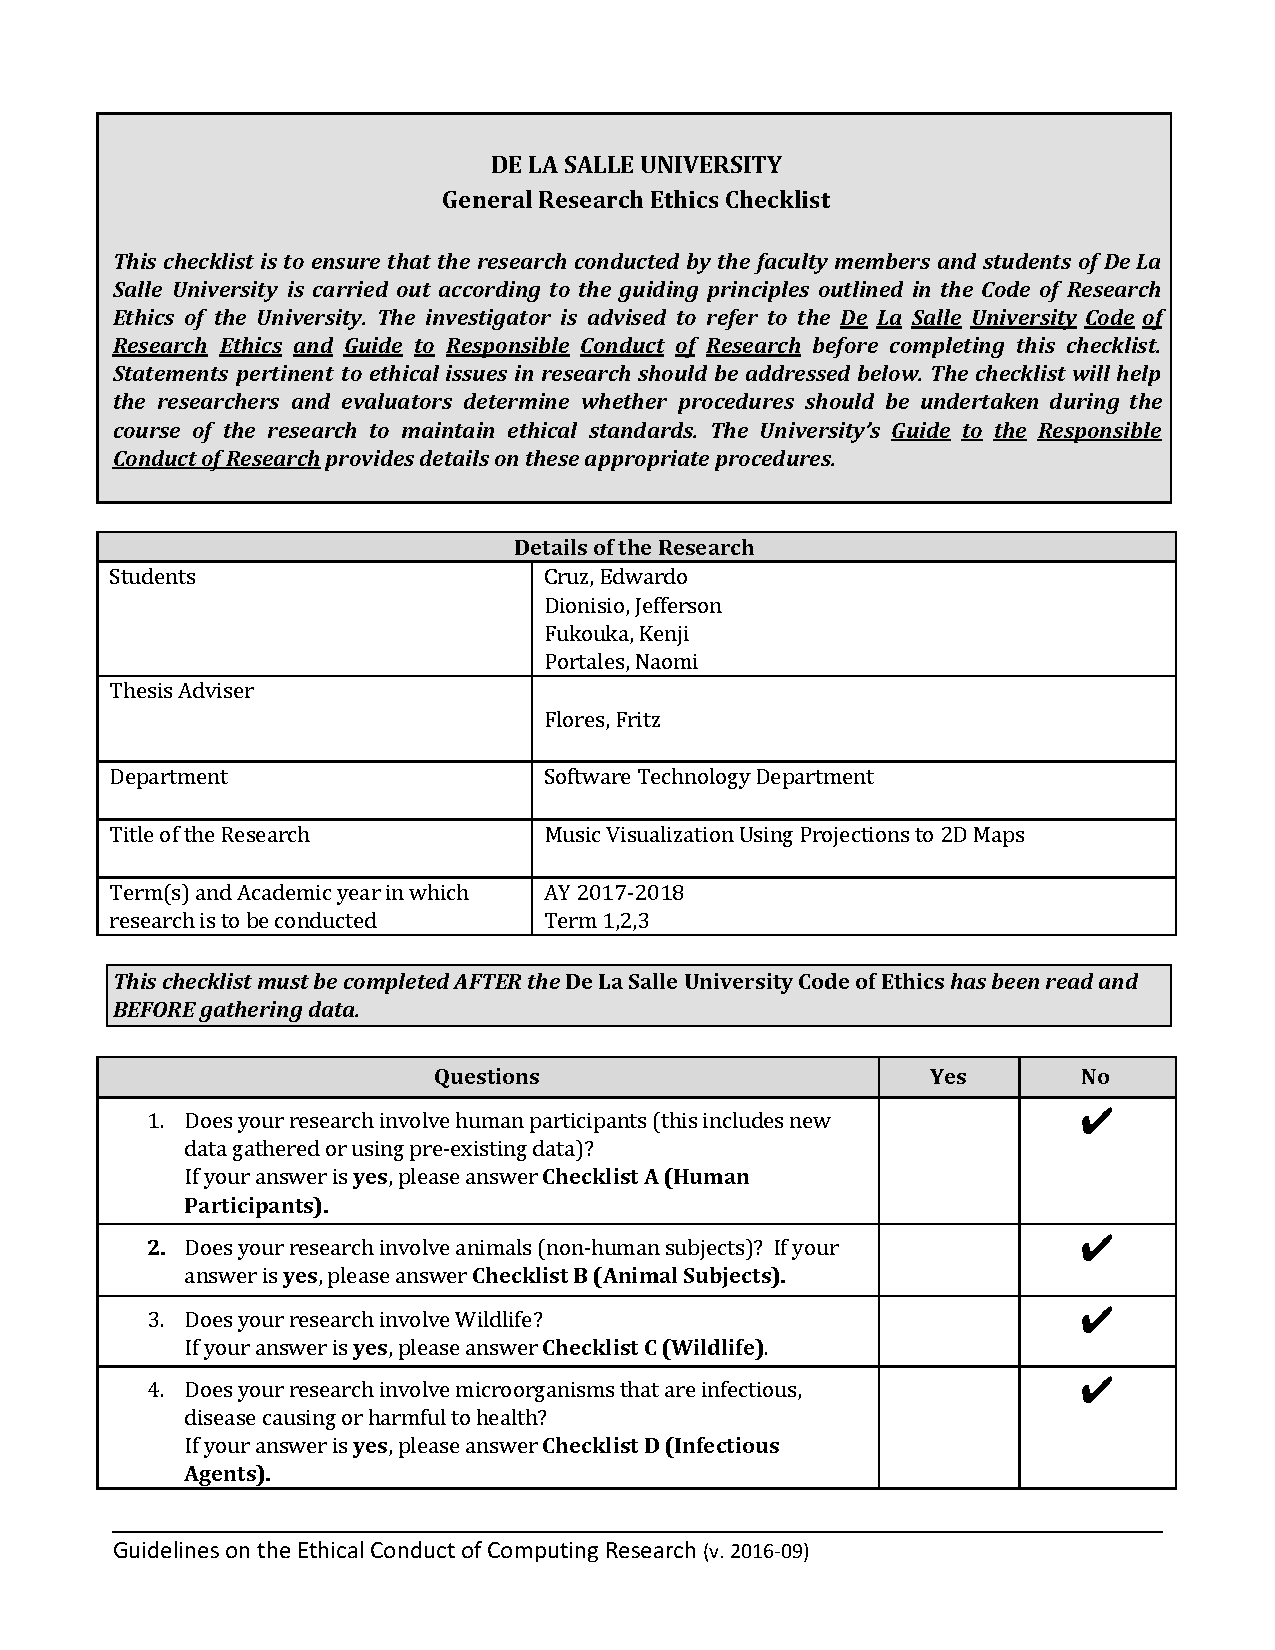
\includepdf[pages=-]{general_checklist.pdf}
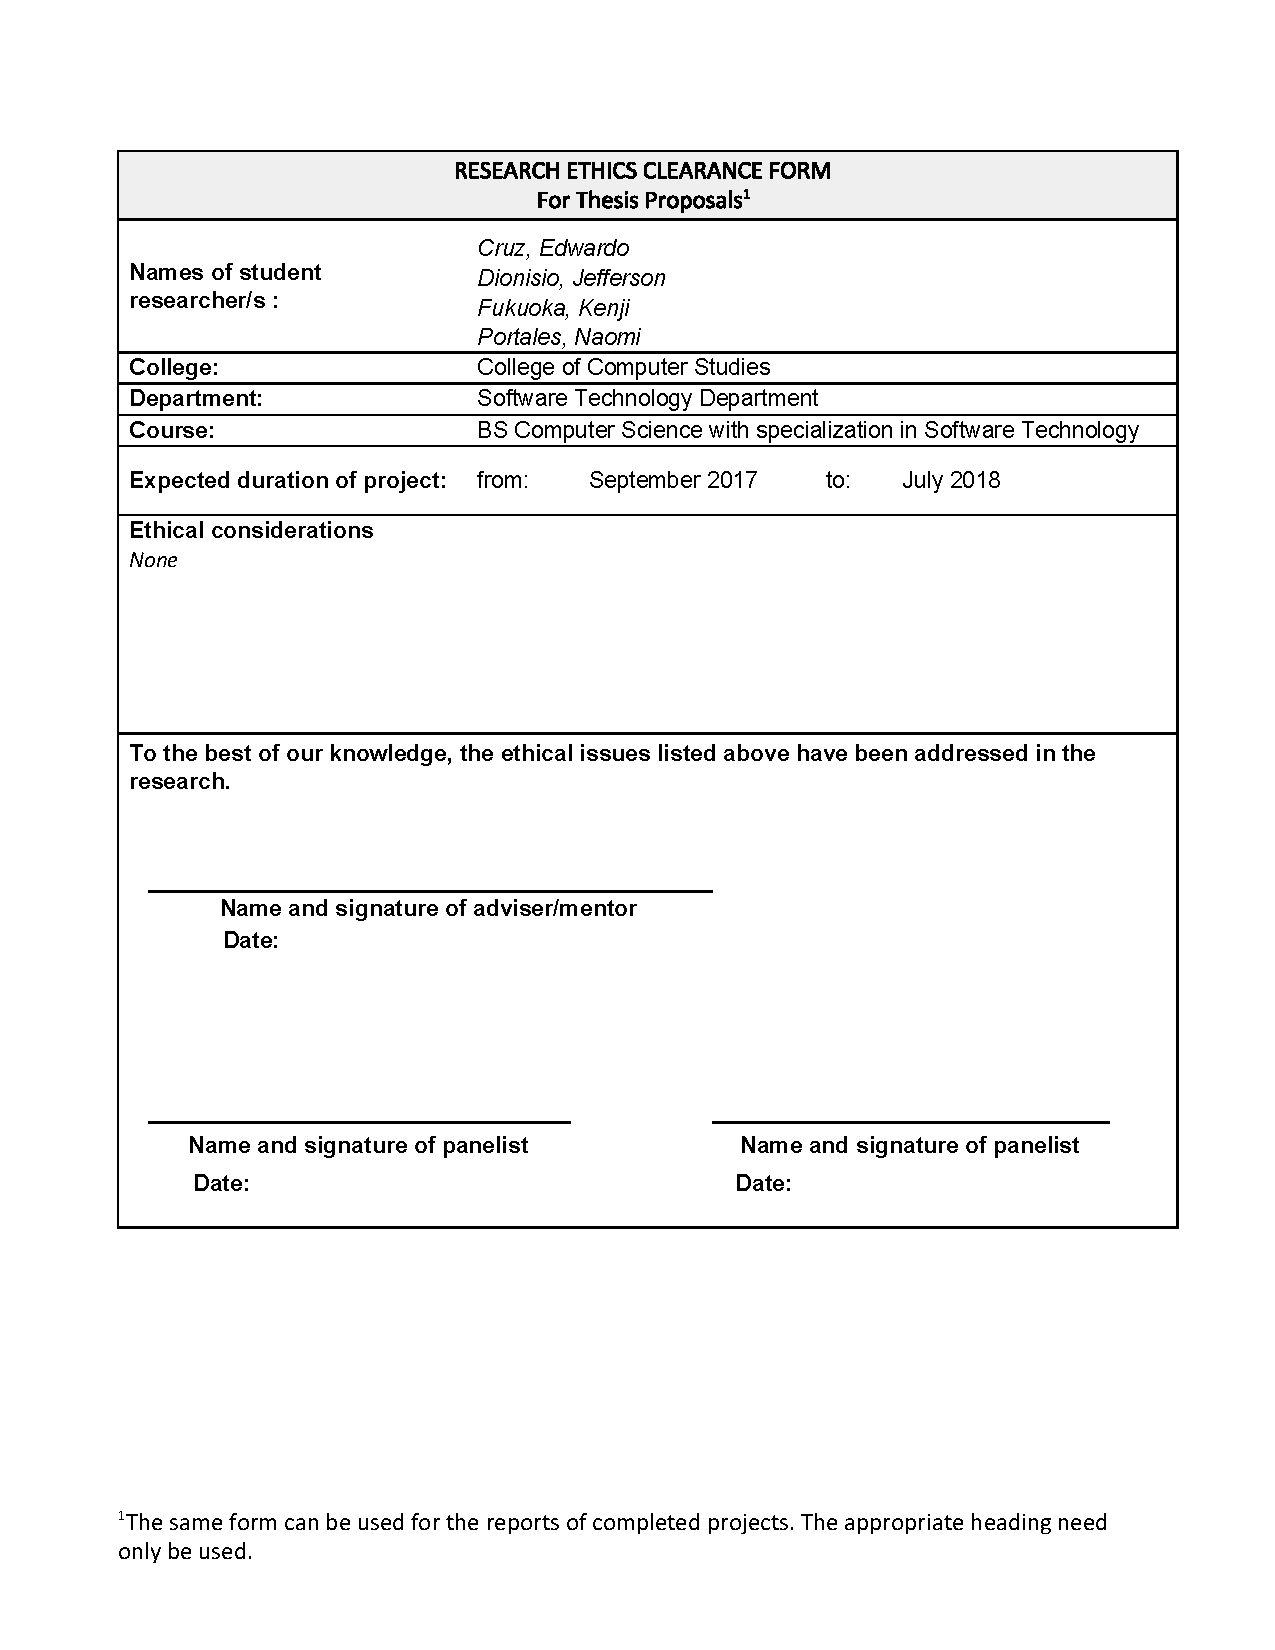
\includepdf[pages=-]{ethics_clearance.pdf}

              %-- includes LaTeX source file for Appendix A
                                                 %-- your job: **CREATE/EDIT** your own source file for the appendices
%%%%%%%%%%%%%%%%%%%%%%%%%%%%%%%%%%%%%%%%%%%%%%%%%%%%%%%%%%%%%%%%%%%%%%%%%%%%%%%%%%%%%%%%%%%%%%%%%%%%%%%
%
%   Filename    : appendix_B.tex 
%
%   Description : This file will contain one of your appendices.
%                 
%%%%%%%%%%%%%%%%%%%%%%%%%%%%%%%%%%%%%%%%%%%%%%%%%%%%%%%%%%%%%%%%%%%%%%%%%%%%%%%%%%%%%%%%%%%%%%%%%%%%%%

\chapter{Theoretical and/or Conceptual Framework}
\label{sec:appendixb}

Discusses the basic framework/foundation the thesis is based on. This section is normally referred to when discussing Scope and Limitations,
and Research Methodology



%%%%%%%%%%%%%%%%%%%%%%%%%%%%%%%%%%%%%%%%%%%%%%%%%%%%%%%%%%%%%%%%%%%%%%%%%%%%%%%%%%%%%%%%%%%%%%%%%%%%%%%
%
%   Filename    : appendix_C.tex
%
%   Description : This file will contain information about your Resource Persons
%                 
%%%%%%%%%%%%%%%%%%%%%%%%%%%%%%%%%%%%%%%%%%%%%%%%%%%%%%%%%%%%%%%%%%%%%%%%%%%%%%%%%%%%%%%%%%%%%%%%%%%%%%

\chapter{Resource Persons}
\label{sec:appendixc}

%
%  Indicate your resource persons here:
%
%	<full name and title, e.g., Dr. Juan de la Cruz>
%	<profession, e.g., faculty>
%	<department, e.g., College of Computer Studies>
%	<name of institution, e.g., De La Salle University>
%	<e-mail address>
%
%

%
%  the following shows 3 examples, replace entries with your own
%
\newcommand{\resperson}[4]{\textbf{#1} \\ #2 \\ #3 \\ \url{#4}\vspace{0.5em}\\}

\resperson{Dr. Firstname1 Lastname1}{Adviser}{College of Computer Studies\\De La Salle University-Manila}{emailaddr@dlsu.edu.ph}
\resperson{Mr. Firstname2 Lastname2}{Role2}{Affiliation2}{emailaddr2@domain.com}
\resperson{Ms. Firstname3 Lastname3}{Role3}{Affiliation3}{emailaddr3@domain.net}



%\bibliographystyle{apacite}       %-- specified APA style for bibliograpy
                                  %-- more details about APA style citation can be found in www.ctan.org/tex-archive/biblio/bibtex/contrib/apacite/

                                  %-- bibliographic entries are handled via bibtex; refer to www.bibtex.org for more details

%%%%%%%%%%%%%%%%%%%%%%%%%%%%%%%%%%%%%%%%%%%%%%%%%%%%%%%%%%%%%%%%%%%%%%%%%%%%%%%%%%%%%%%%%%%%%%%%%%%%%%
%
%   Filename    : appendix_A.tex 
%
%   Description : This file is one of the appendices. 
%                 
%%%%%%%%%%%%%%%%%%%%%%%%%%%%%%%%%%%%%%%%%%%%%%%%%%%%%%%%%%%%%%%%%%%%%%%%%%%%%%%%%%%%%%%%%%%%%%%%%%%%%%

\textbf{\Huge Appendix A}
\bigskip

\textbf{\LARGE Research Ethics Documents}

\bigskip
This section contains all documents related to research ethics.

\newpage
\setlength{\voffset}{0cm}
\setlength{\hoffset}{0cm}

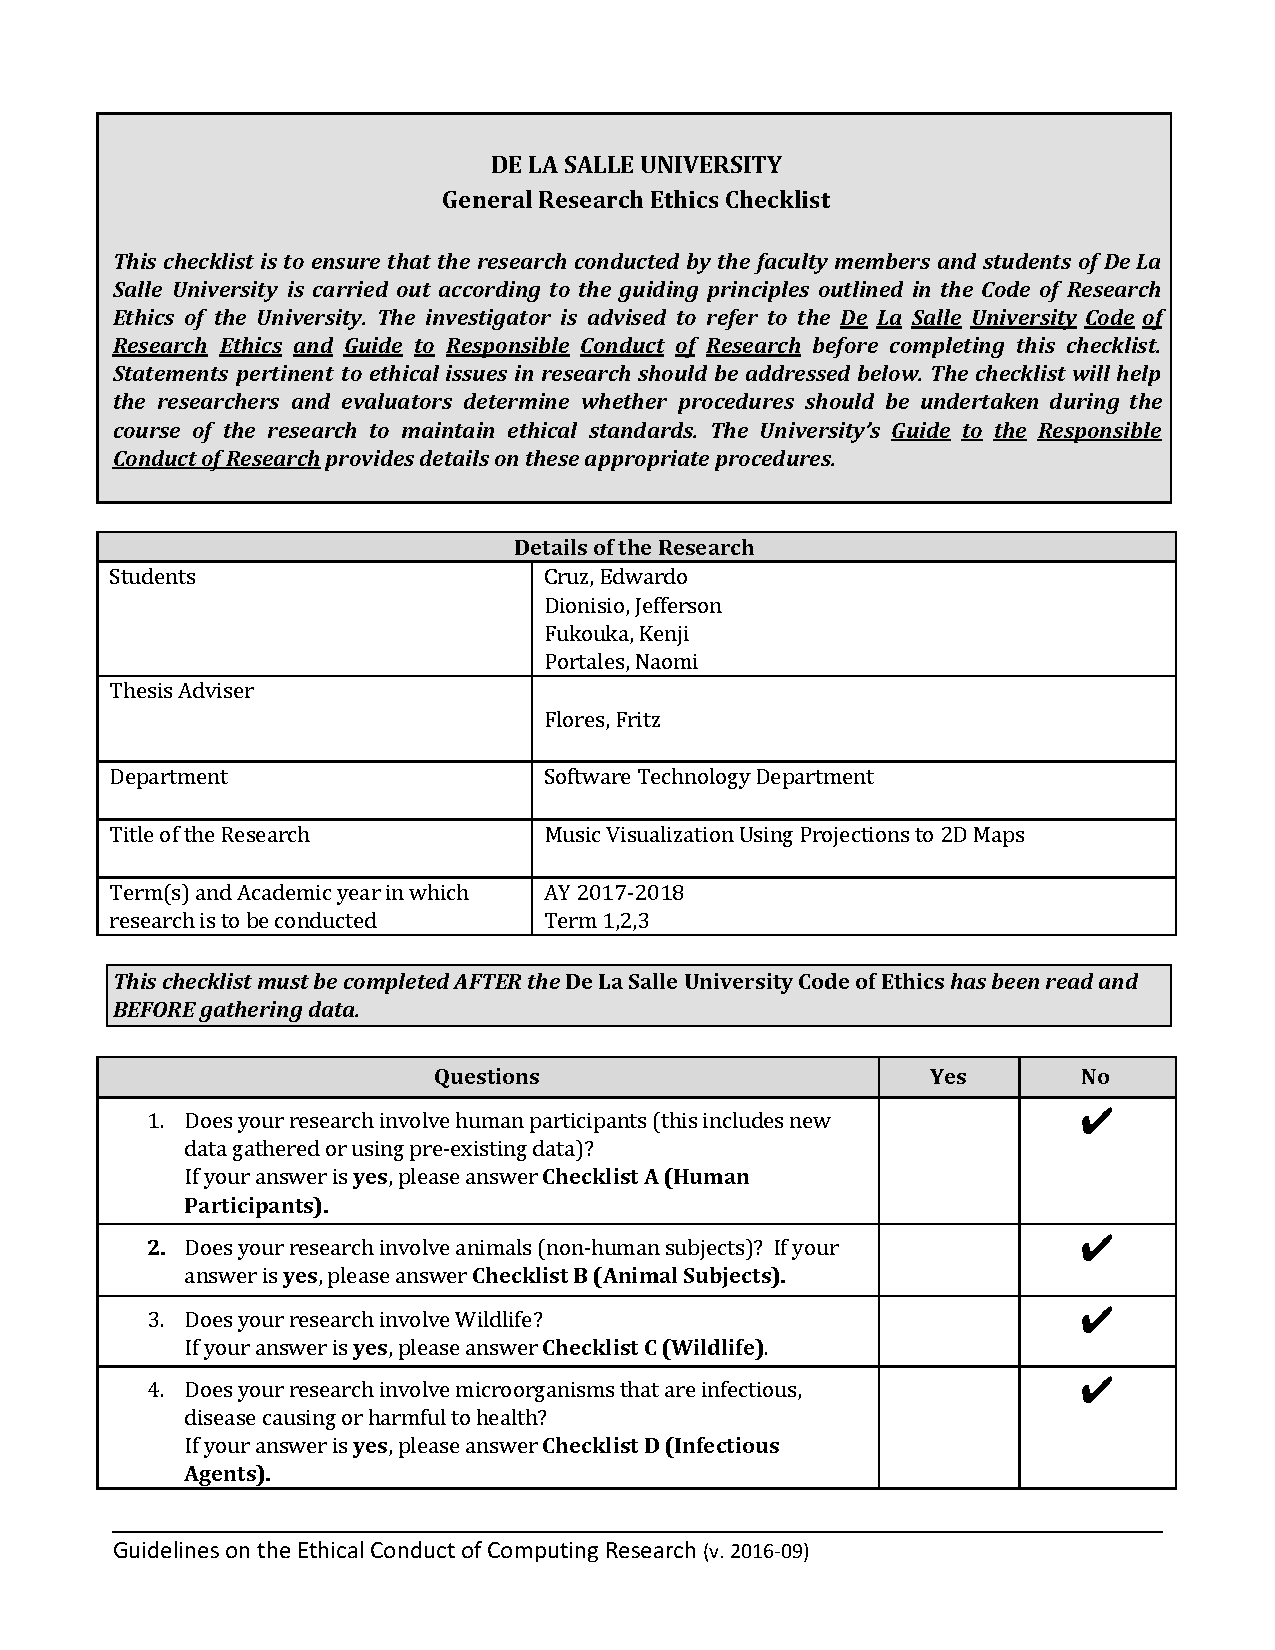
\includepdf[pages=-]{general_checklist.pdf}
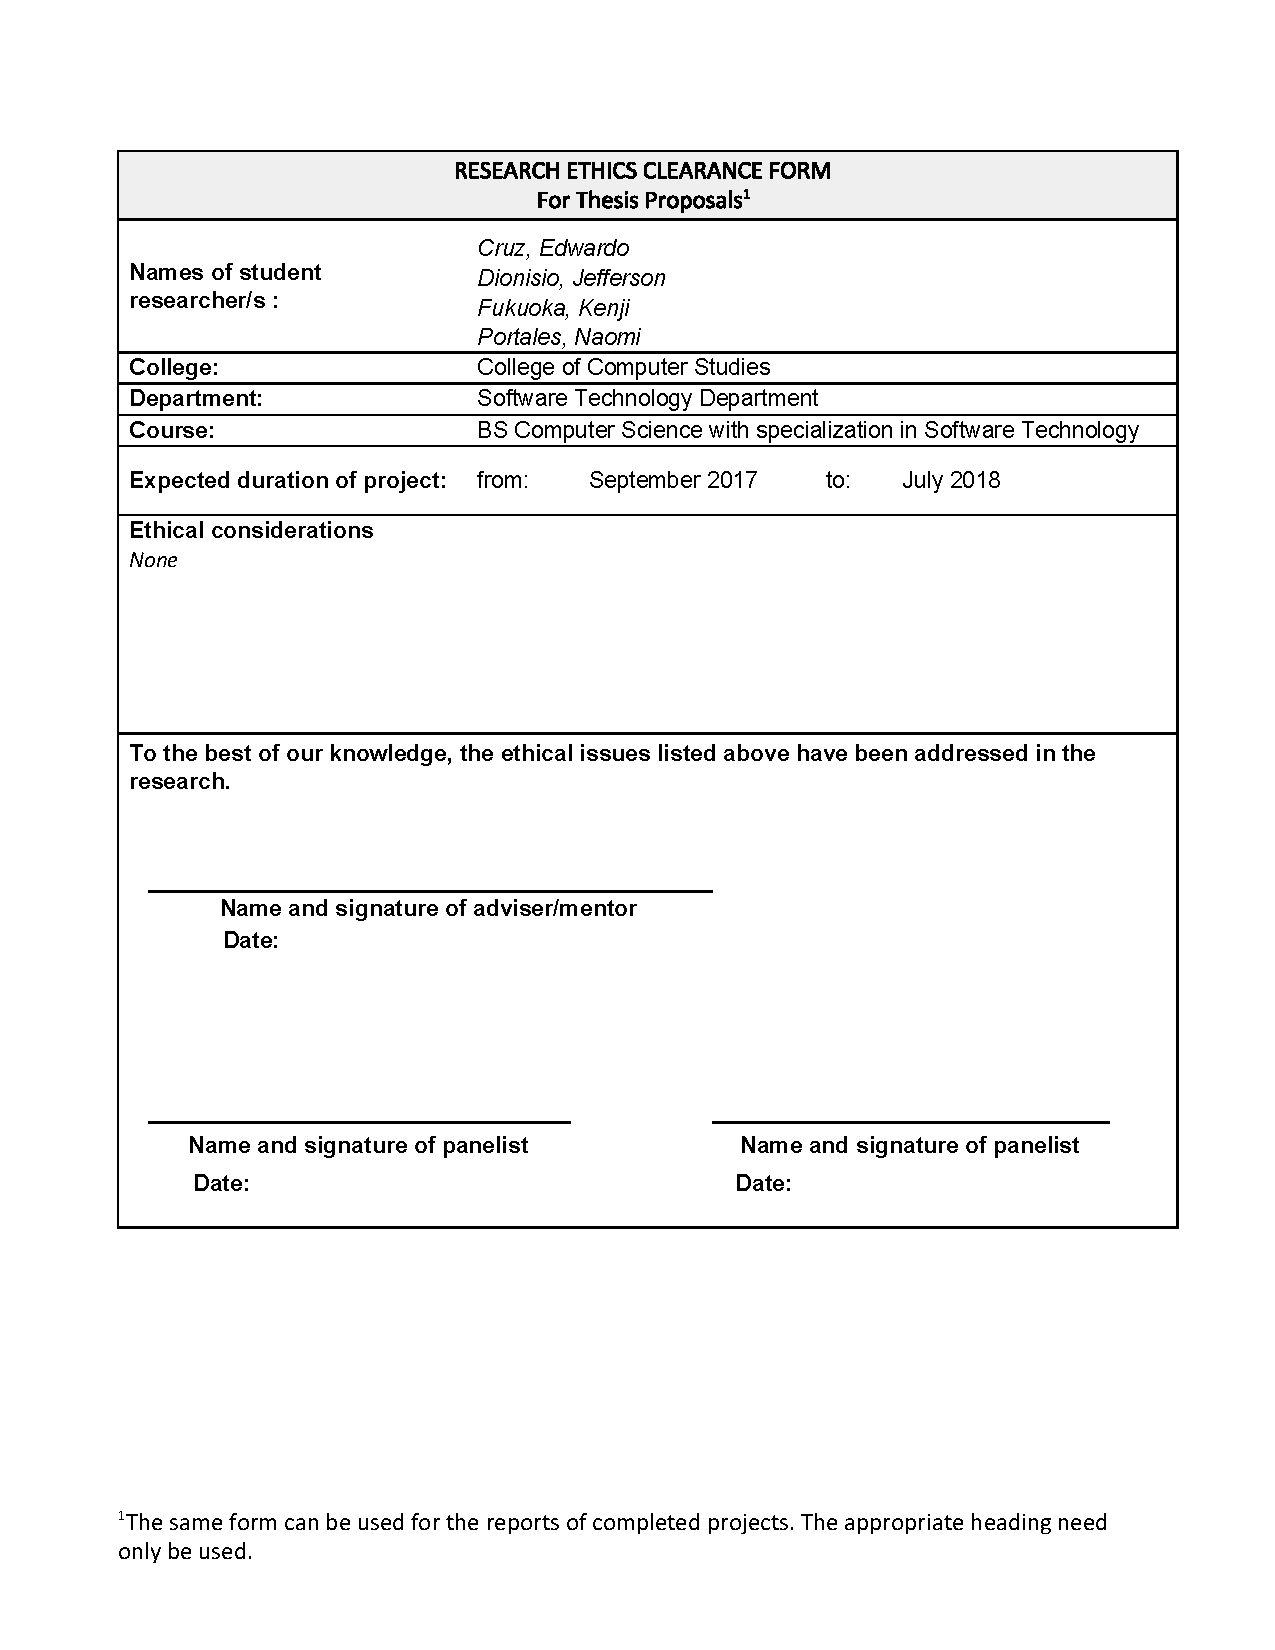
\includepdf[pages=-]{ethics_clearance.pdf}


%%%%%%%%%%%%%%%%%%%%%%%%%%%%%%%%%%%%%%%%%%%%%%%%%%%%%%%%%%%%%%%%%%%%%%%%%%%%%%%%%%%%%%%%%%%%%%%%%%%%%%
%
%   Filename    : appendix_B.tex 
%
%   Description : This file will contain one of your appendices.
%                 
%%%%%%%%%%%%%%%%%%%%%%%%%%%%%%%%%%%%%%%%%%%%%%%%%%%%%%%%%%%%%%%%%%%%%%%%%%%%%%%%%%%%%%%%%%%%%%%%%%%%%%

\chapter{Theoretical and/or Conceptual Framework}
\label{sec:appendixb}

Discusses the basic framework/foundation the thesis is based on. This section is normally referred to when discussing Scope and Limitations,
and Research Methodology



%%%%%%%%%%%%%%%%%%%%%%%%%%%%%%%%%%%%%%%%%%%%%%%%%%%%%%%%%%%%%%%%%%%%%%%%%%%%%%%%%%%%%%%%%%%%%%%%%%%%%%
%
%   Filename    : appendix_C.tex
%
%   Description : This file will contain information about your Resource Persons
%                 
%%%%%%%%%%%%%%%%%%%%%%%%%%%%%%%%%%%%%%%%%%%%%%%%%%%%%%%%%%%%%%%%%%%%%%%%%%%%%%%%%%%%%%%%%%%%%%%%%%%%%%

\chapter{Resource Persons}
\label{sec:appendixc}

%
%  Indicate your resource persons here:
%
%	<full name and title, e.g., Dr. Juan de la Cruz>
%	<profession, e.g., faculty>
%	<department, e.g., College of Computer Studies>
%	<name of institution, e.g., De La Salle University>
%	<e-mail address>
%
%

%
%  the following shows 3 examples, replace entries with your own
%
\newcommand{\resperson}[4]{\textbf{#1} \\ #2 \\ #3 \\ \url{#4}\vspace{0.5em}\\}

\resperson{Dr. Firstname1 Lastname1}{Adviser}{College of Computer Studies\\De La Salle University-Manila}{emailaddr@dlsu.edu.ph}
\resperson{Mr. Firstname2 Lastname2}{Role2}{Affiliation2}{emailaddr2@domain.com}
\resperson{Ms. Firstname3 Lastname3}{Role3}{Affiliation3}{emailaddr3@domain.net}


%%%%%%%%%%%%%%%%%%%%%%%%%%%%%%%%%%%%%%%%%%%%%%%%%%%%%%%%%%%%%%%%%%%%%%%%%%%%%%%%%%%%%%%%%%%%%%%%%%%%%%
%
%   Filename    : appendix_C.tex
%
%   Description : This file will contain information about your Resource Persons
%                 
%%%%%%%%%%%%%%%%%%%%%%%%%%%%%%%%%%%%%%%%%%%%%%%%%%%%%%%%%%%%%%%%%%%%%%%%%%%%%%%%%%%%%%%%%%%%%%%%%%%%%%

\textbf{\Huge Appendix D}
\bigskip

\textbf{\LARGE Symphony Map from Azcarraga \& Flores (2016)'s SOMphony}

\bigskip
This section contains an image sample of a symphony map

\begin{figure}[h]
\centering
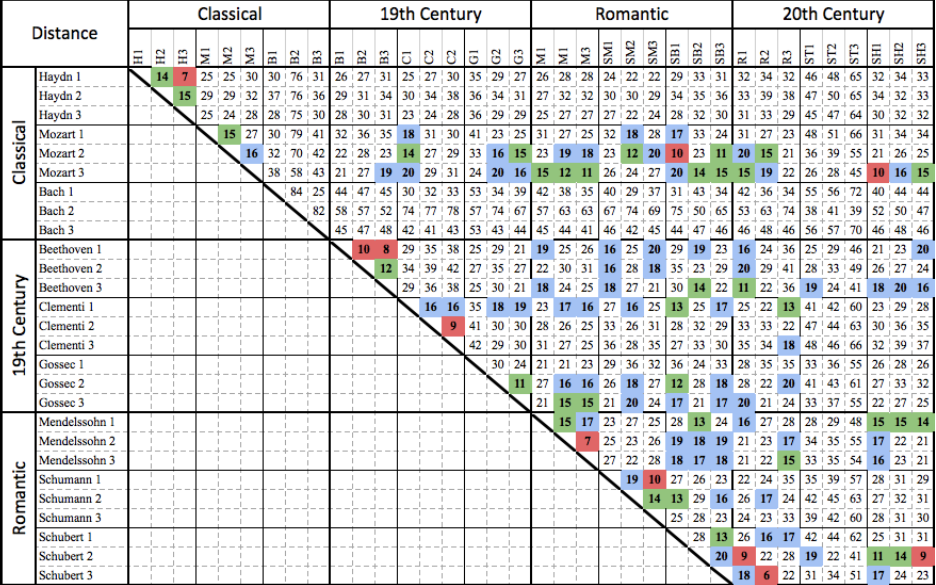
\includegraphics[scale=0.7]{somphony_composers}
\end{figure}


%%%%%%%%%%%%%%%%%%%%%%%%%%%%%%%%%%%%%%%%%%%%%%%%%%%%%%%%%%%%%%%%%%%%%%%%%%%%%%%%%%%%%%%%%%%%%%%%%%%%%%
%
%   Filename    : appendix_C.tex
%
%   Description : This file will contain information about your Resource Persons
%                 
%%%%%%%%%%%%%%%%%%%%%%%%%%%%%%%%%%%%%%%%%%%%%%%%%%%%%%%%%%%%%%%%%%%%%%%%%%%%%%%%%%%%%%%%%%%%%%%%%%%%%%

\textbf{\Huge Appendix E}
\bigskip

\textbf{\LARGE Resource persons}

\bigskip
\textbf{Mr. Fritz Kevin S. Flores}

Adviser

College of Computer Studies

{De La Salle University-Manila}

fritz.flores$@$dlsu.edu.ph


\textbf{\Huge Appendix F}
\bigskip

\textbf{\LARGE t-SNE Results}

\bigskip
This section contains all the t-SNE plots that resulted from this research.


\begin{figure}[!htb]
\caption{Per Period Plot}
\centering
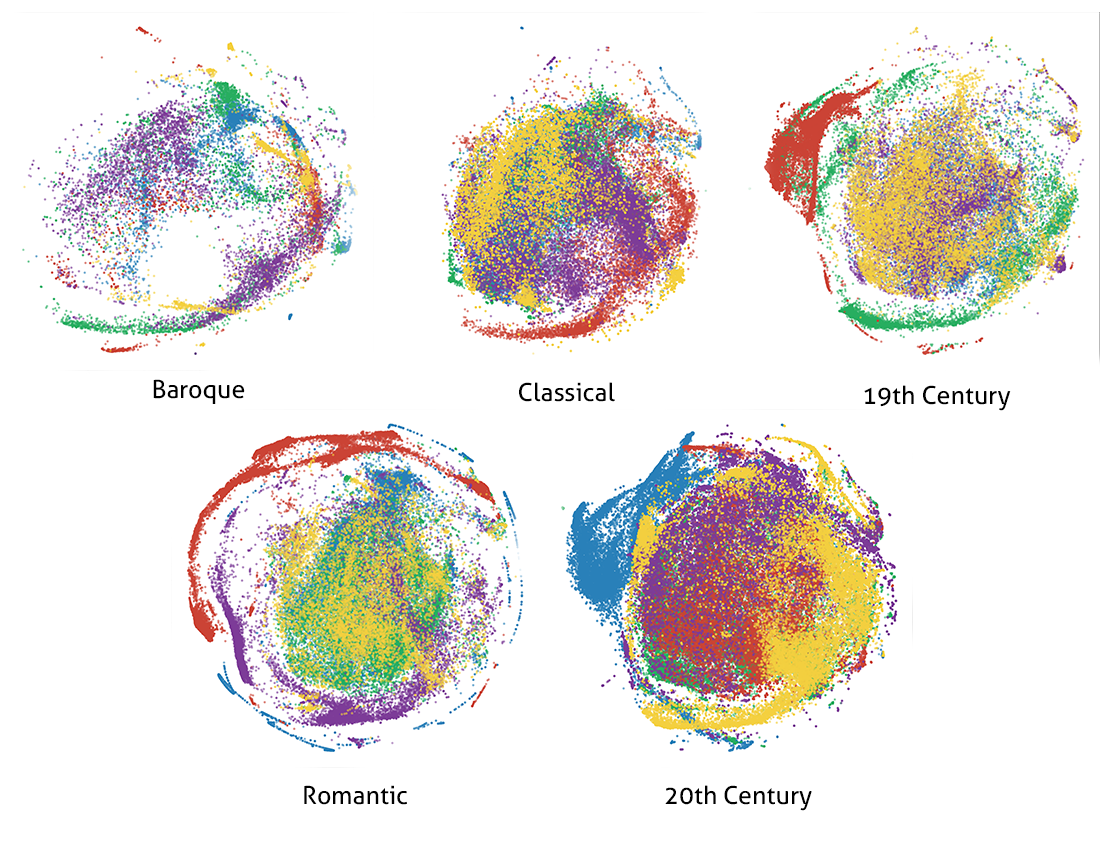
\includegraphics[scale=0.5]{per_era}
\end{figure}

\begin{figure}[!htb]
\caption{Per Composer Plot}
\centering
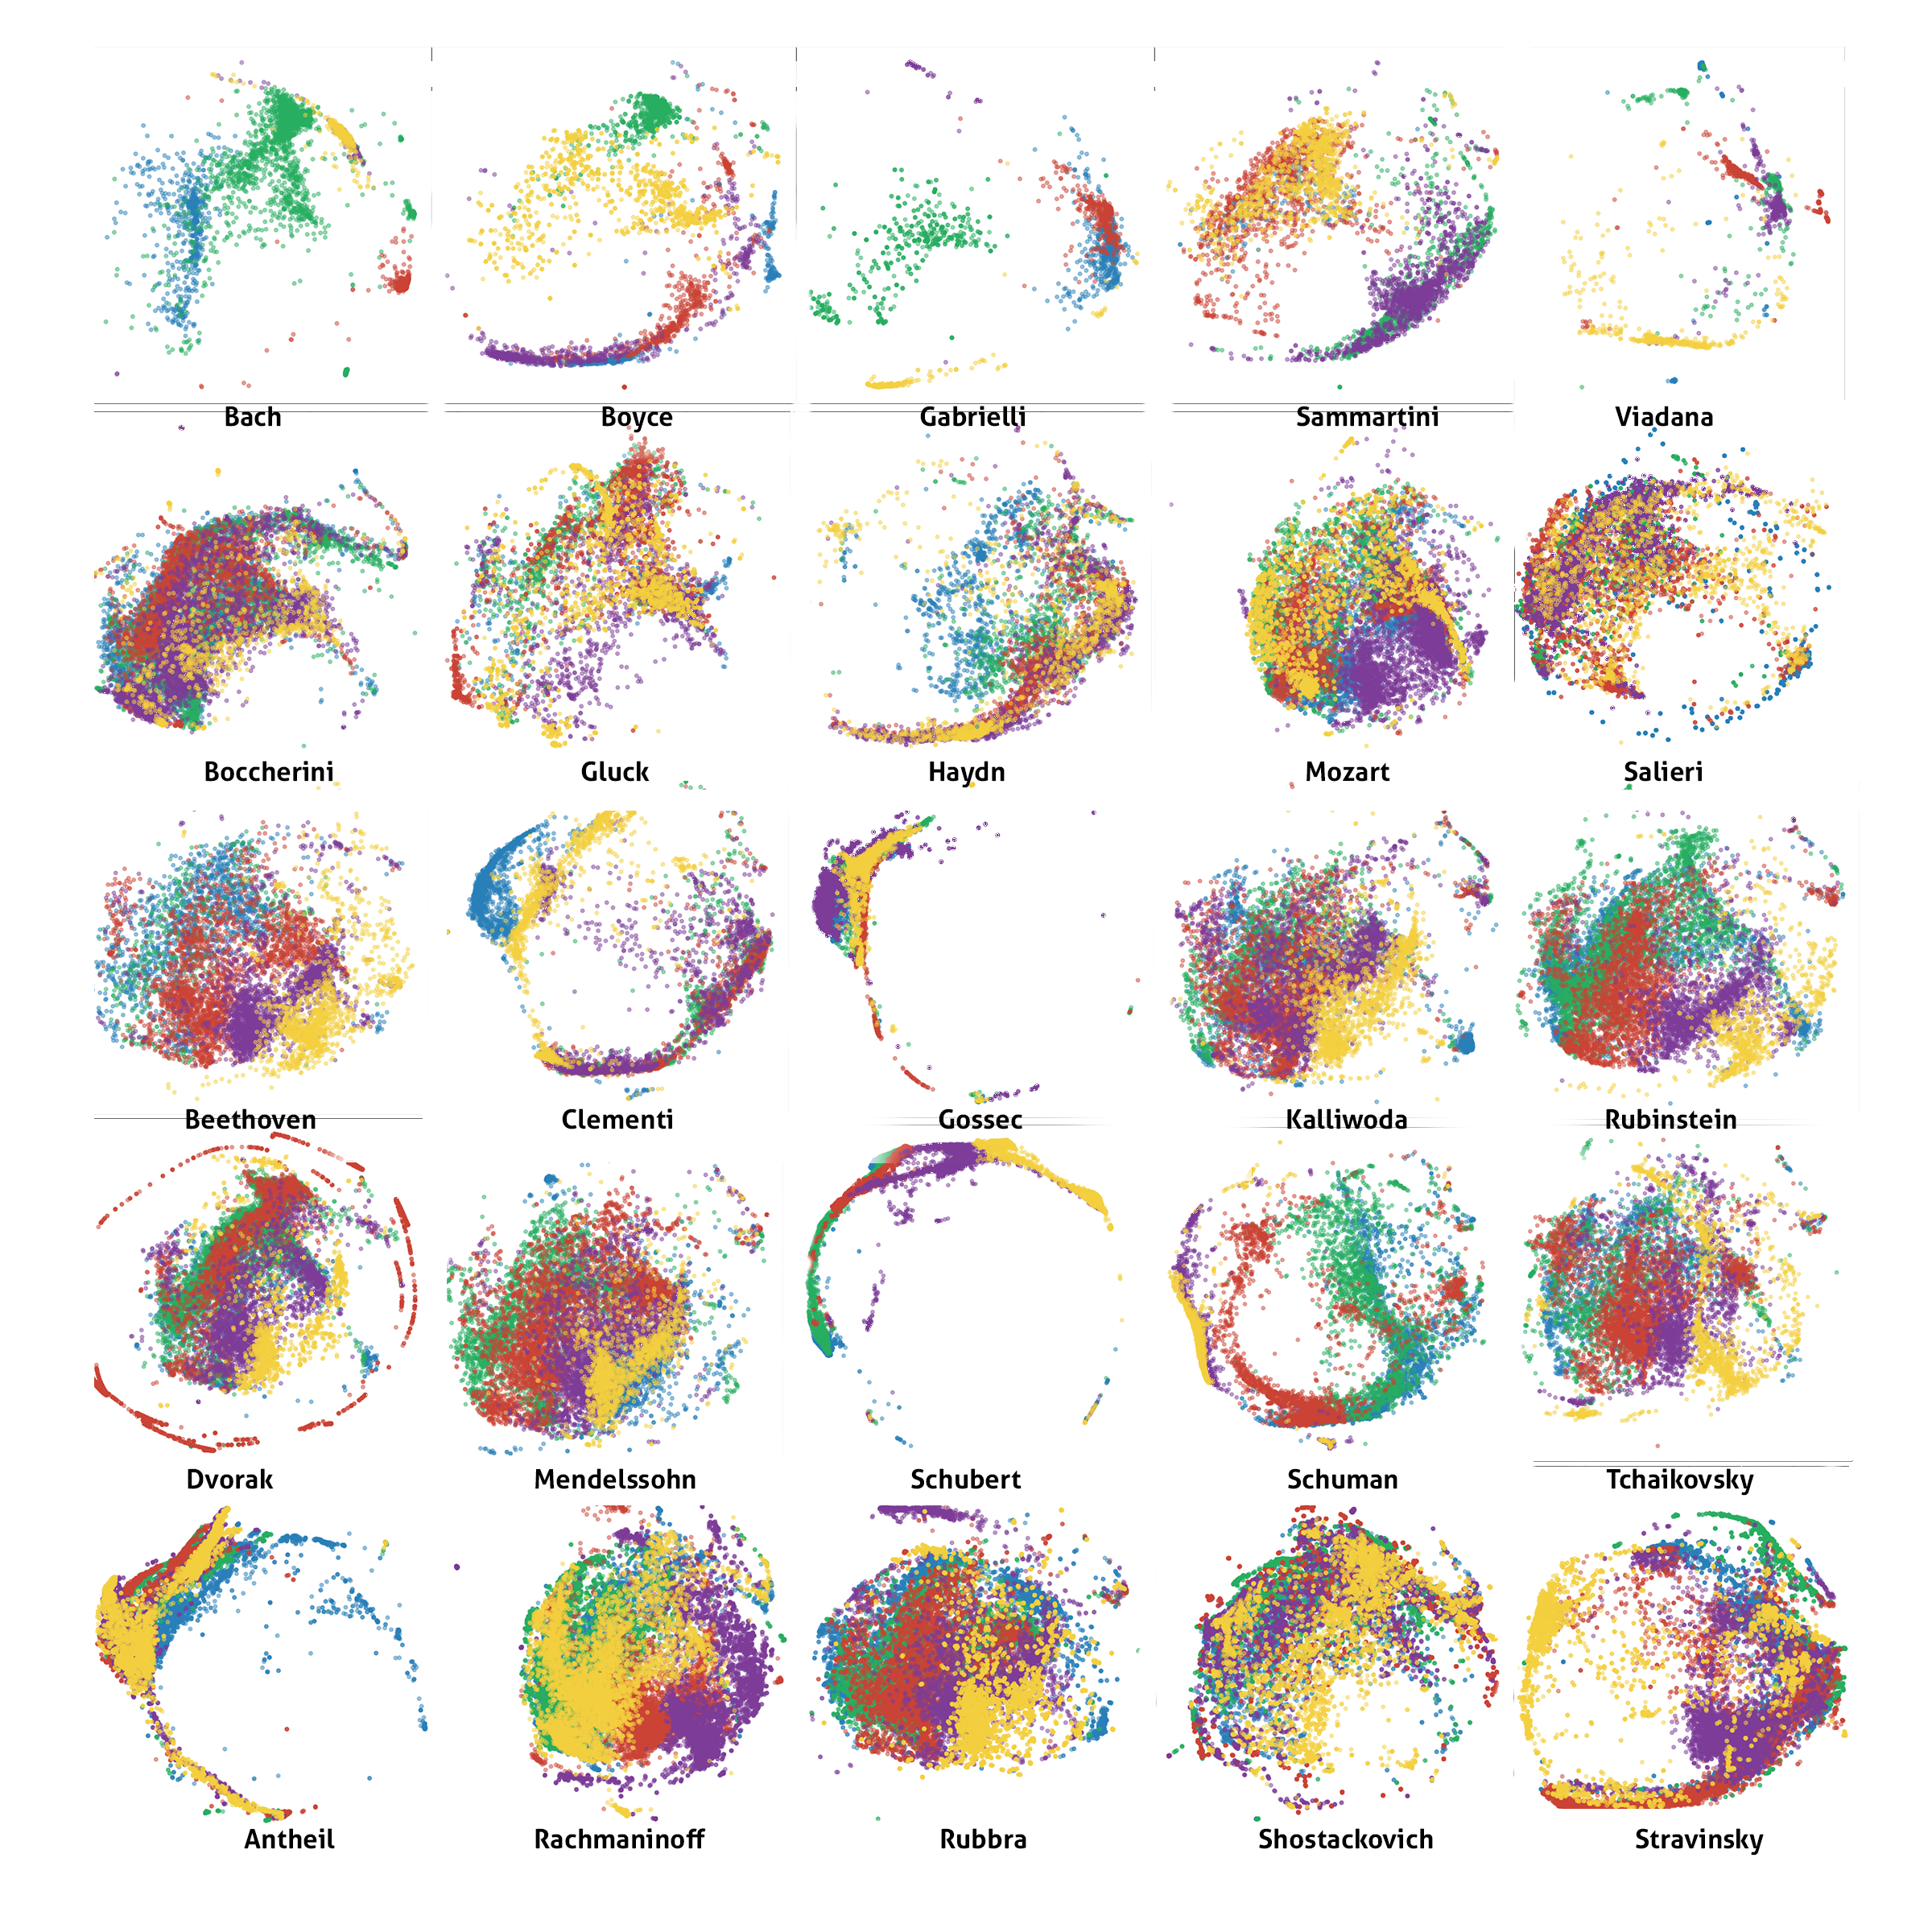
\includegraphics[scale=0.25]{per_composer}
\end{figure}

\begin{figure}
\centering
\begin{minipage}{.5\textwidth}
  \captionof{figure}{Baroque Period}
  \centering
  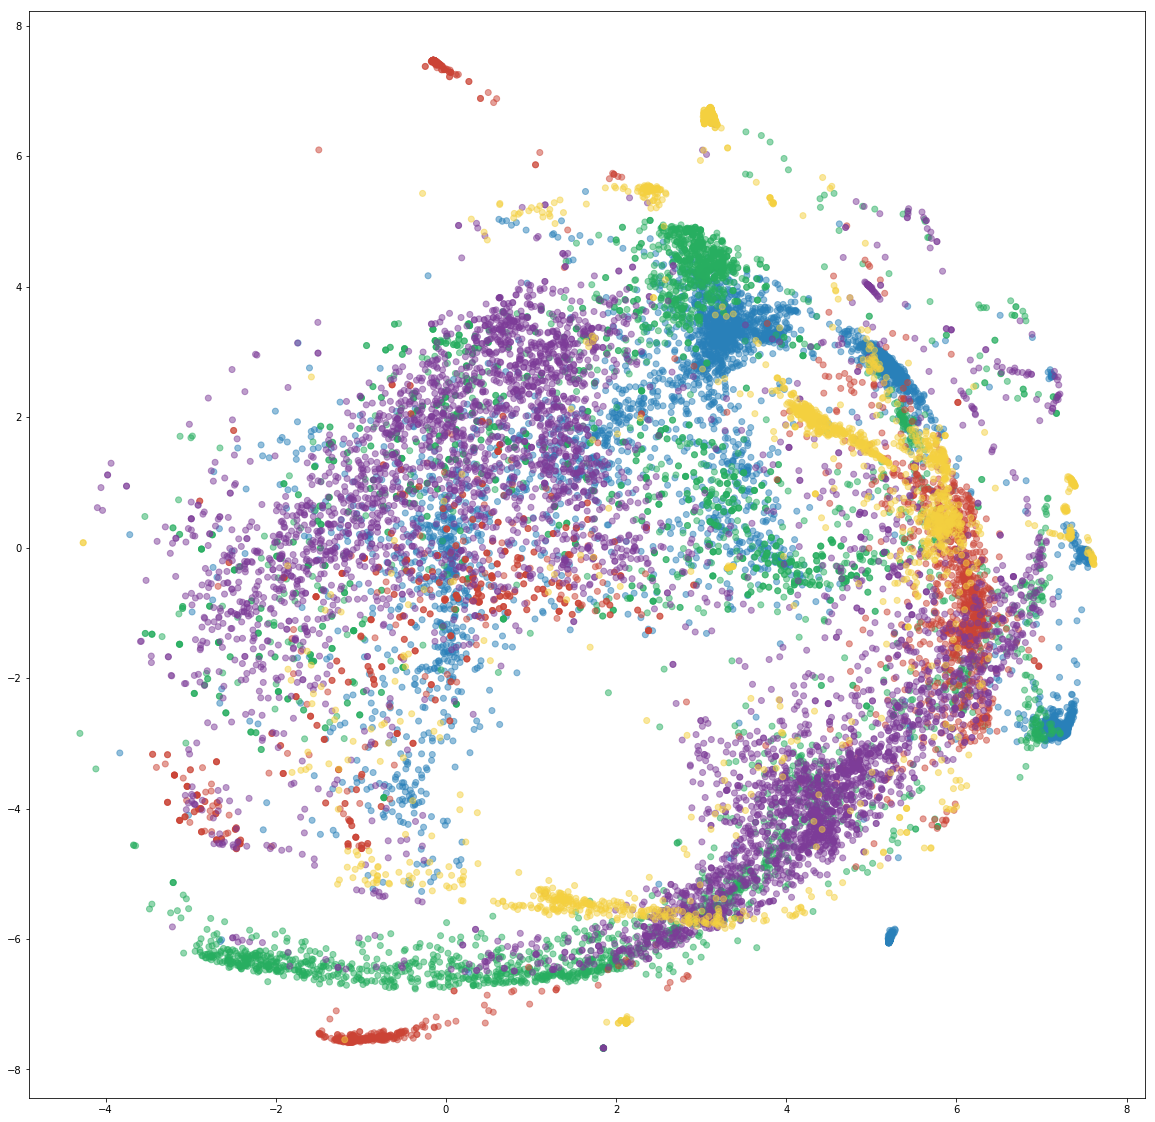
\includegraphics[scale=0.15]{era1}
  \label{fig:test1}
\end{minipage}%
\begin{minipage}{.5\textwidth}
  \captionof{figure}{Classical Period}
  \centering
  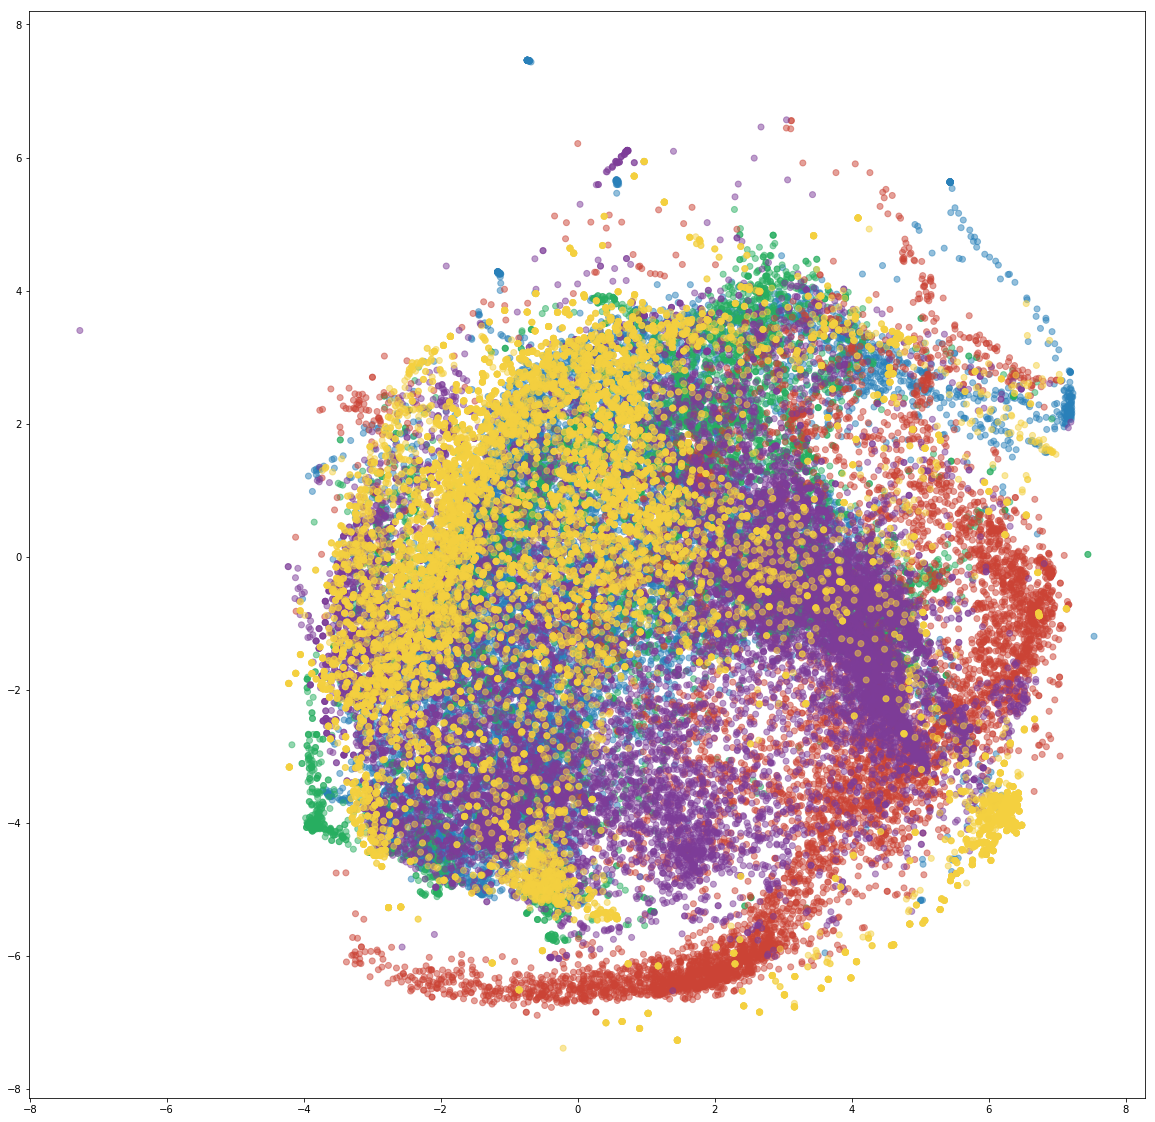
\includegraphics[scale=0.15]{era2}
  \label{fig:test2}
\end{minipage}
\end{figure}

\begin{figure}
\centering
\begin{minipage}{.5\textwidth}
  \captionof{figure}{19th Century}
  \centering
  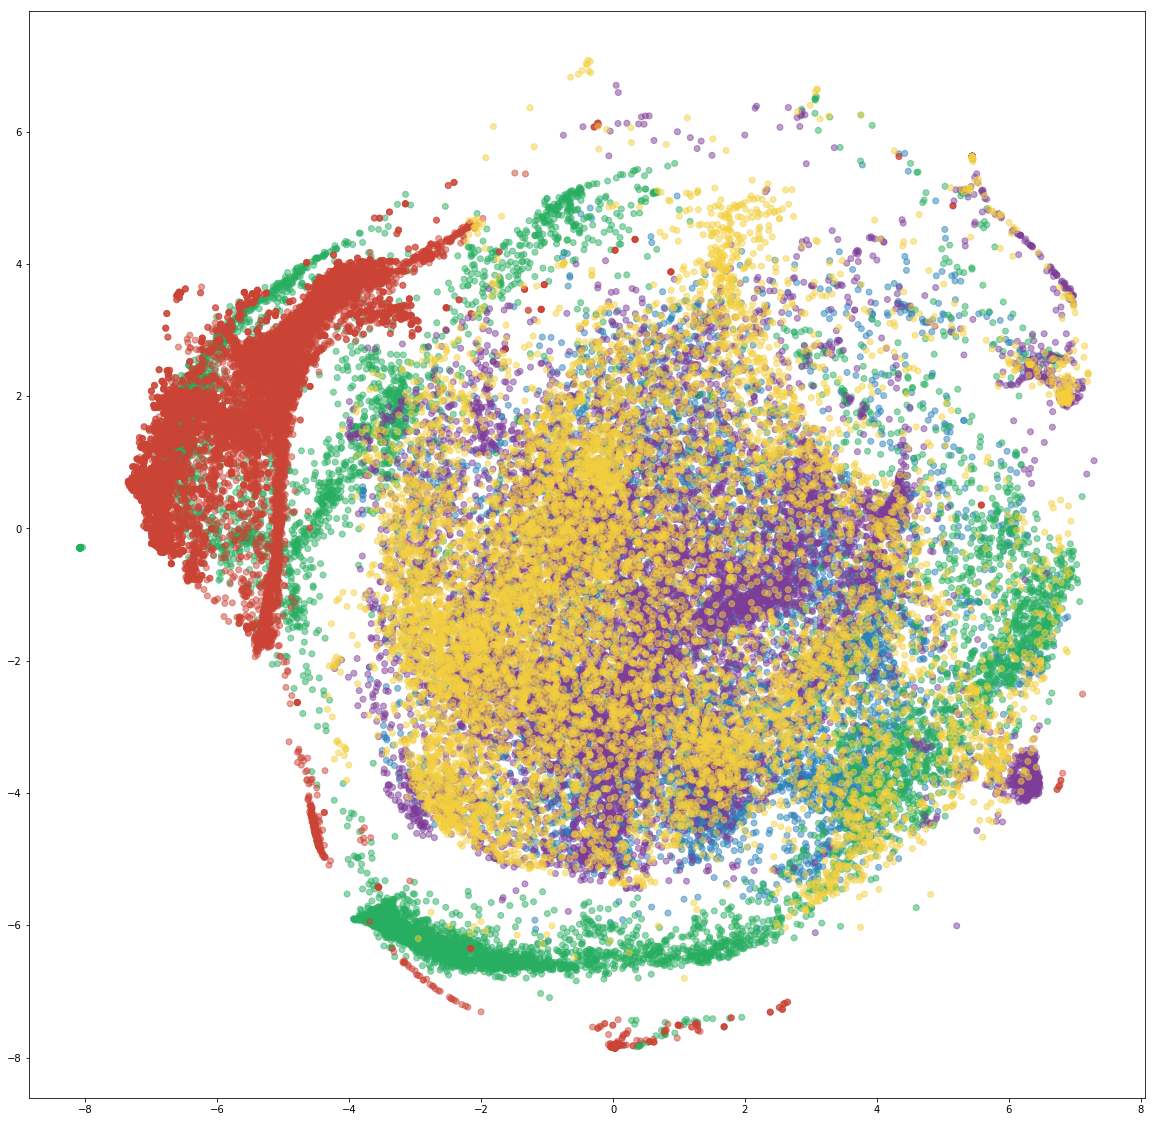
\includegraphics[scale=0.15]{era3}
  \label{fig:test1}
\end{minipage}%
\begin{minipage}{.5\textwidth}
  \captionof{figure}{Romantic Period}
  \centering
  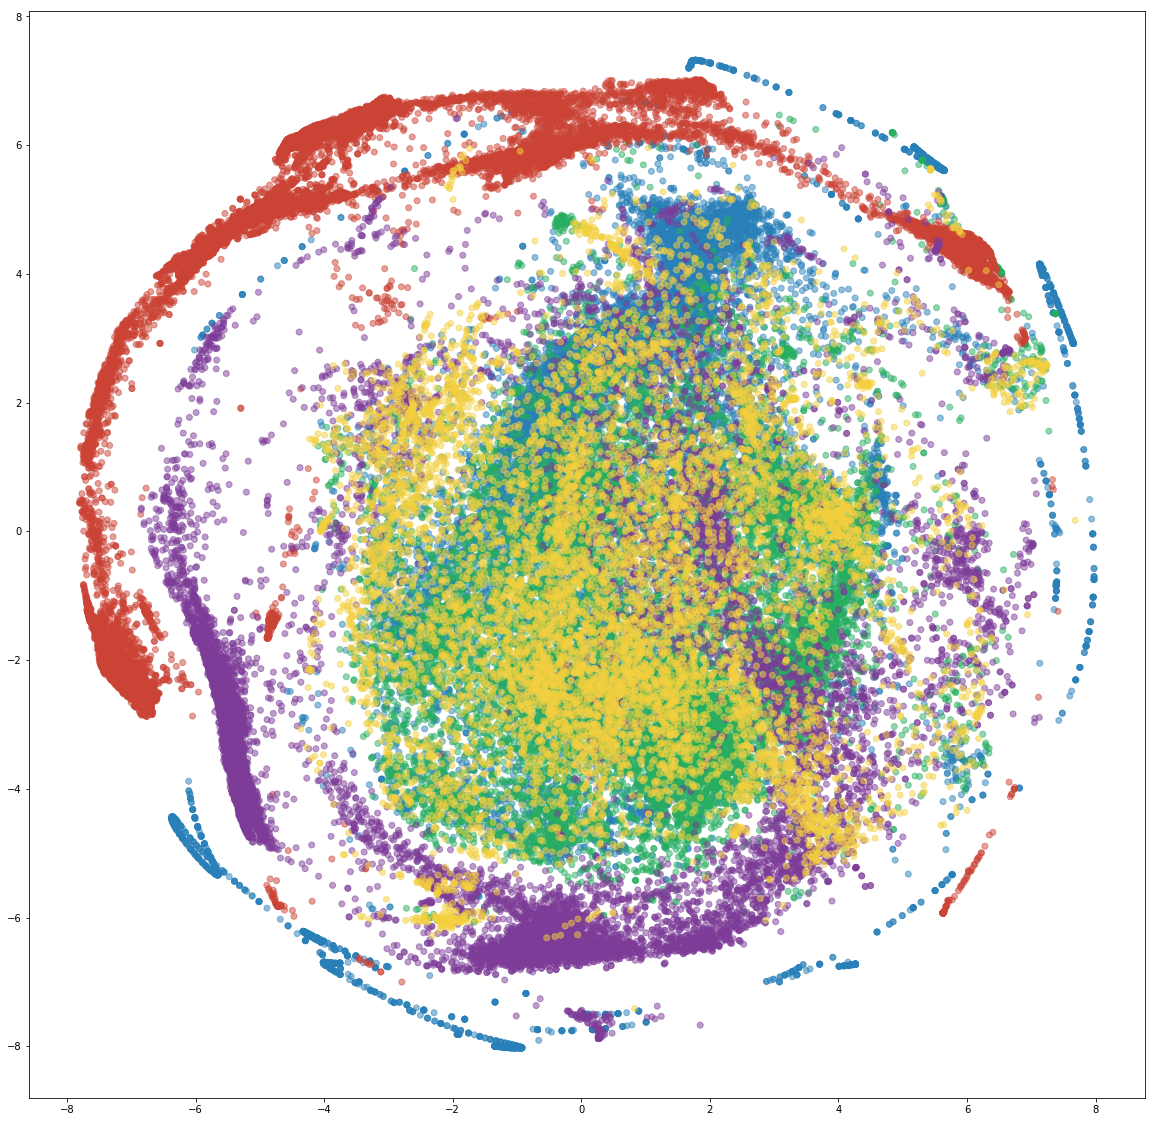
\includegraphics[scale=0.15]{era4}
  \label{fig:test2}
\end{minipage}
\end{figure}

\begin{figure}[h]
\caption{20th Century}
\centering
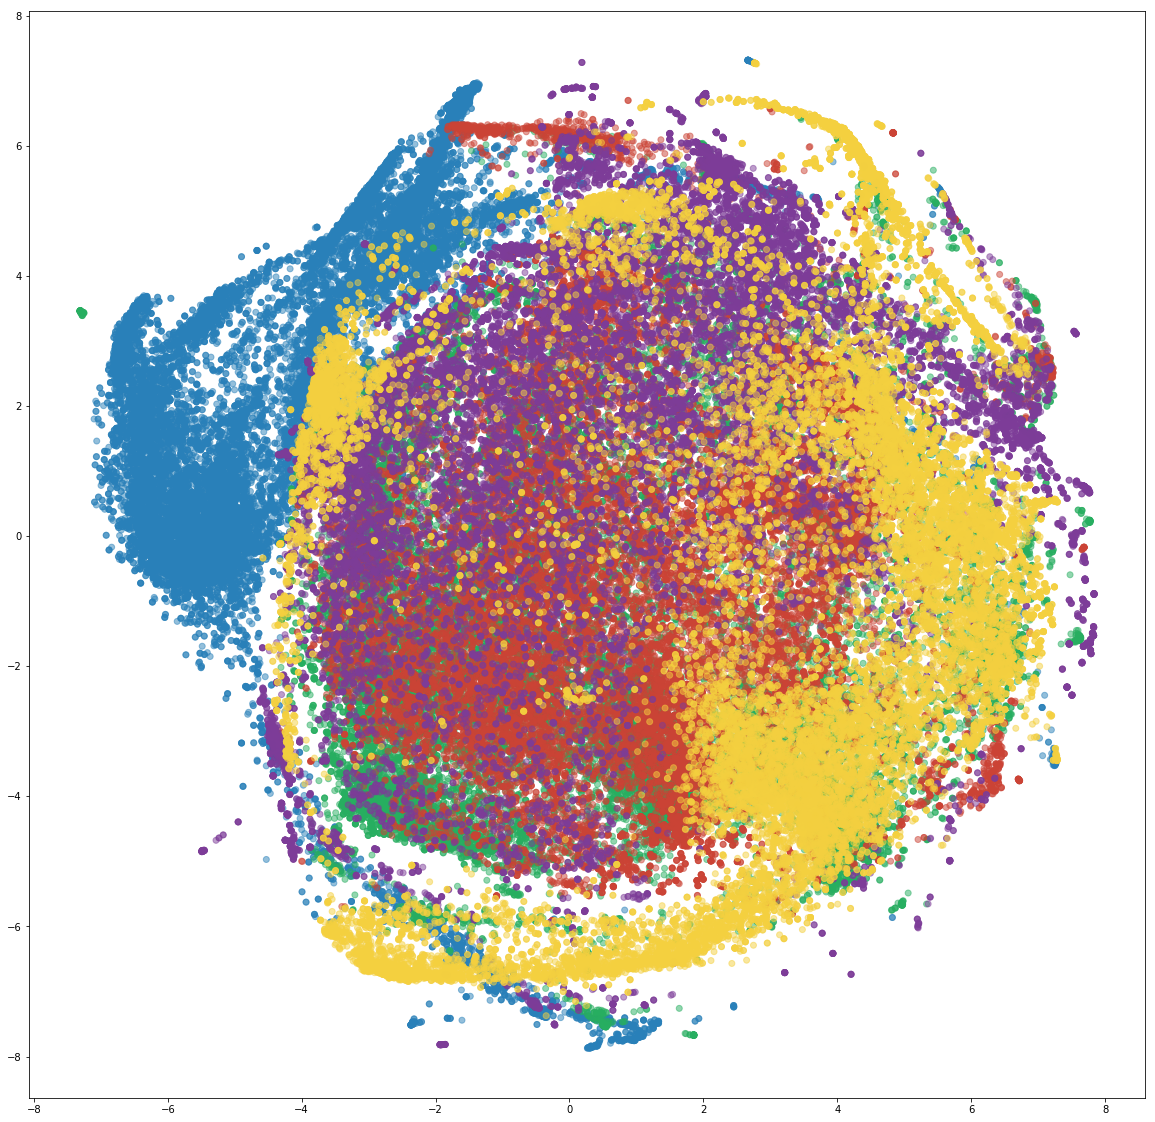
\includegraphics[scale=0.15]{era5}
\end{figure}

\begin{figure}
\centering
\begin{minipage}{.5\textwidth}
  \captionof{figure}{Baroque: Bach}
  \centering
  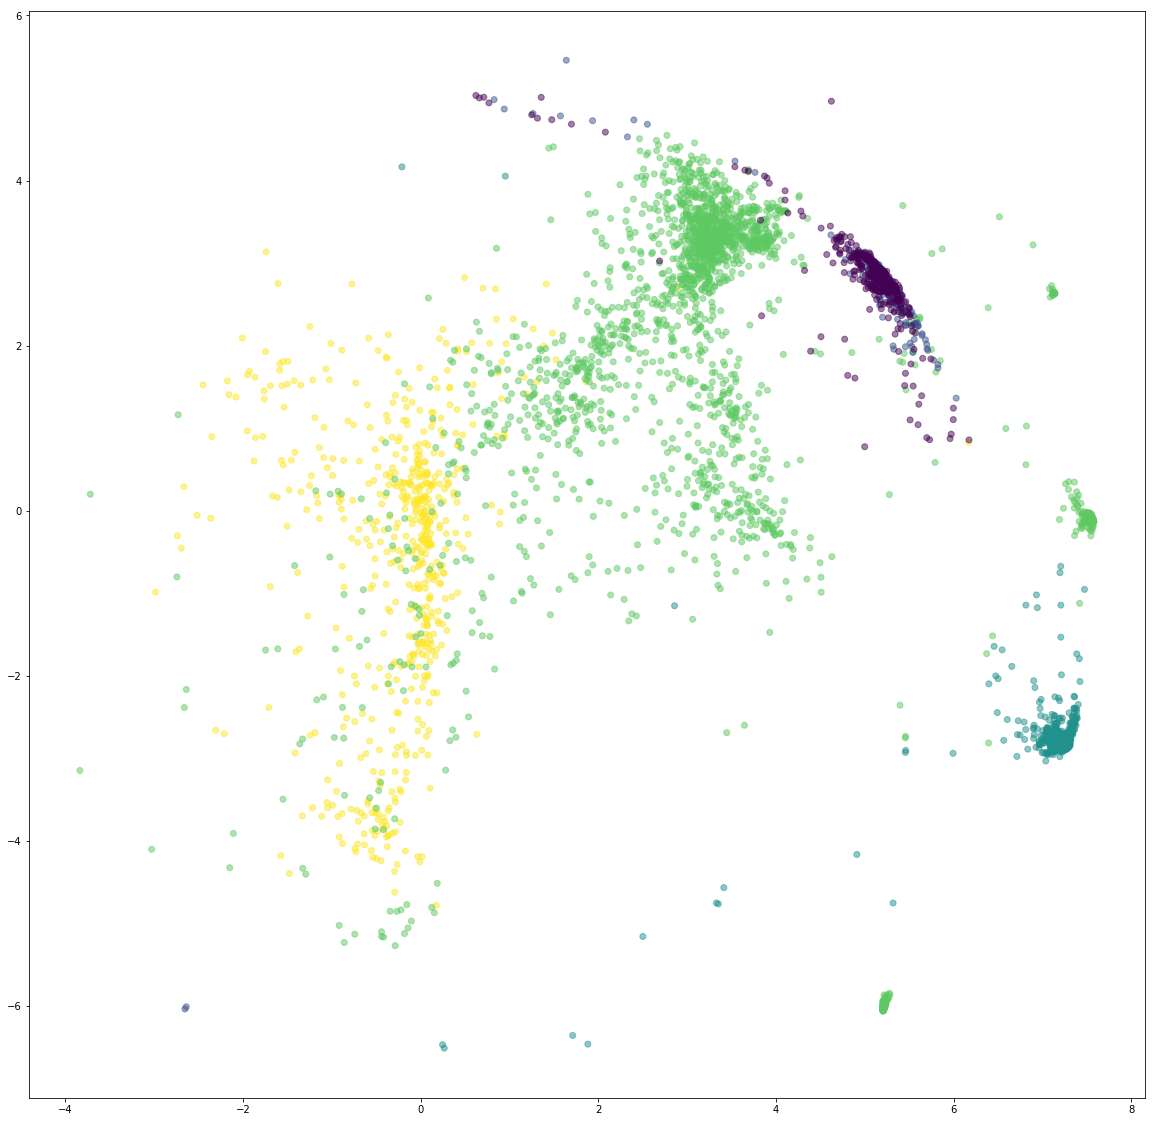
\includegraphics[scale=0.15]{P1C1}
  \label{fig:test1}
\end{minipage}%
\begin{minipage}{.5\textwidth}
  \captionof{figure}{Baroque: Boyce}
  \centering
  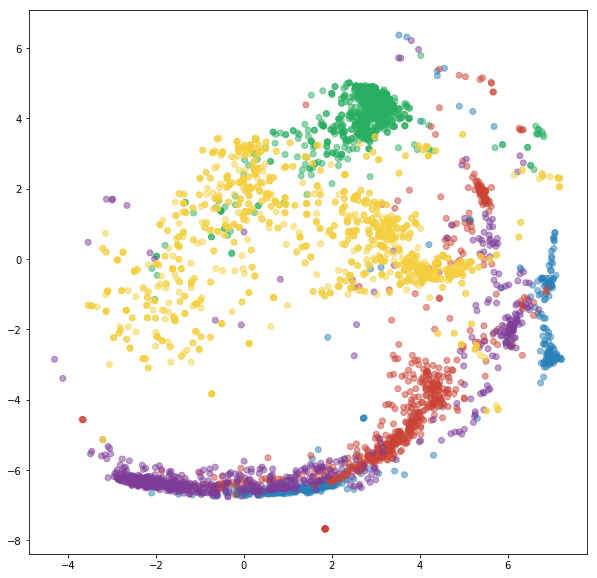
\includegraphics[scale=0.15]{P1C2}
  \label{fig:test2}
\end{minipage}
\end{figure}

\begin{figure}
\centering
\begin{minipage}{.5\textwidth}
  \captionof{figure}{Baroque: Gabrieli}
  \centering
  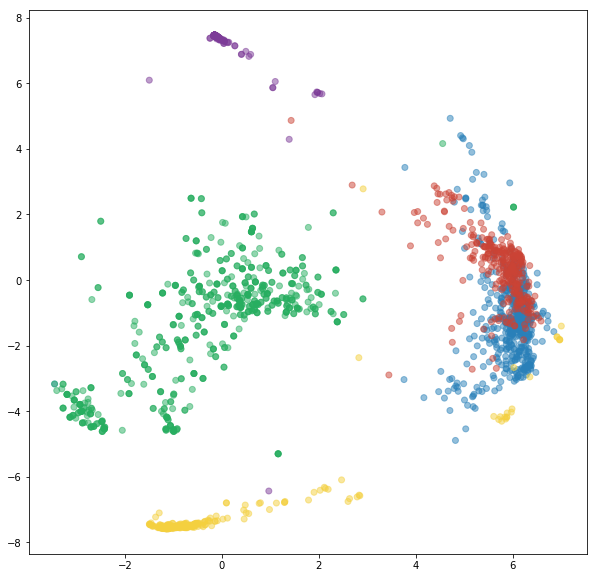
\includegraphics[scale=0.15]{P1C3}
  \label{fig:test1}
\end{minipage}%
\begin{minipage}{.5\textwidth}
  \captionof{figure}{Baroque: Sammartini}
  \centering
  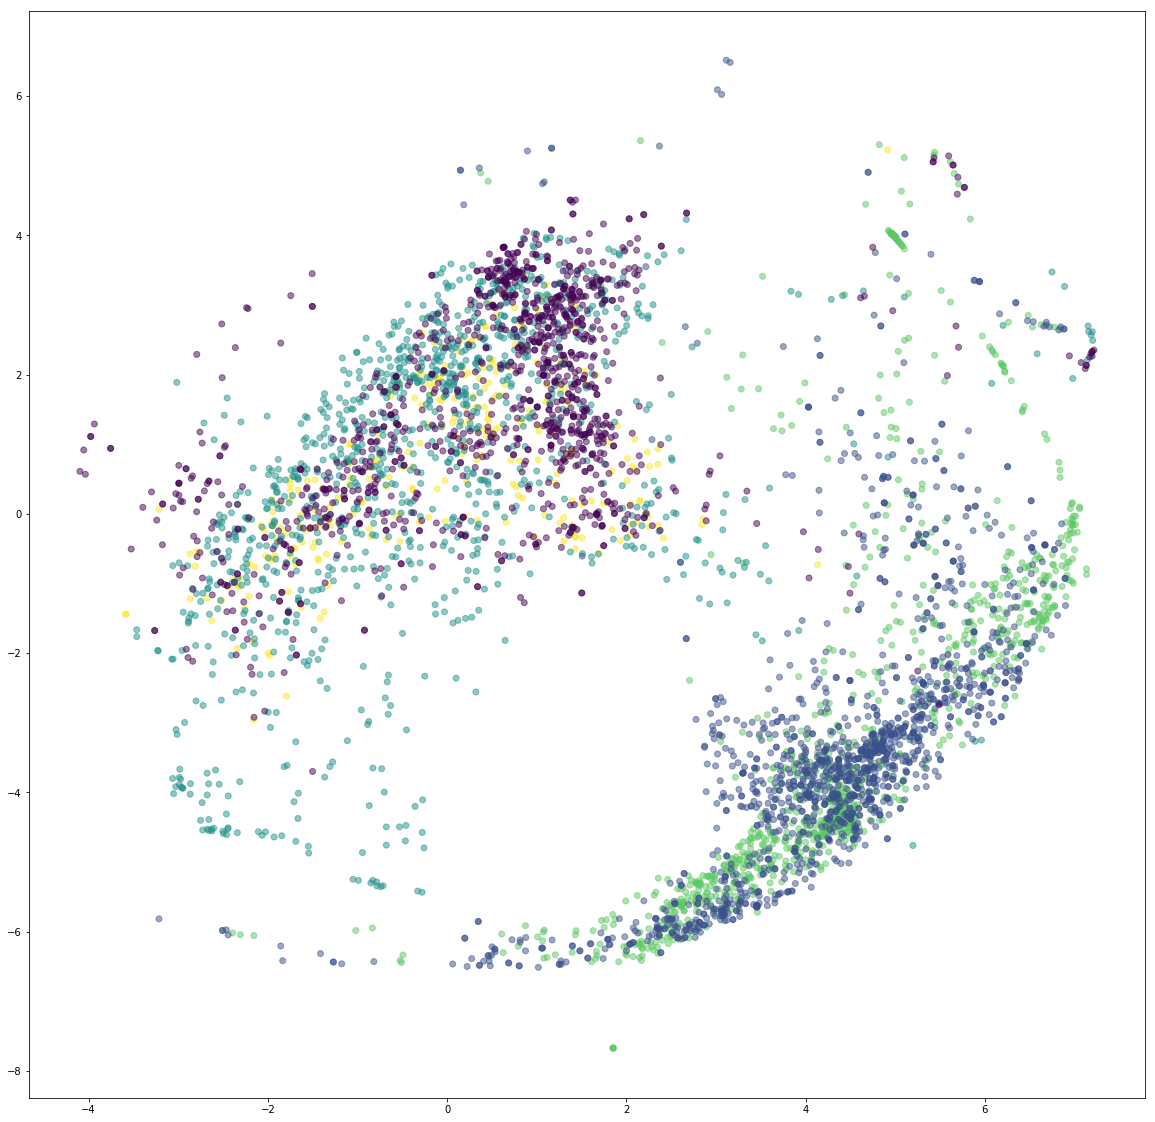
\includegraphics[scale=0.15]{P1C4}
  \label{fig:test2}
\end{minipage}
\end{figure}

\begin{figure}[h]
\caption{Baroque: Viadana}
\centering
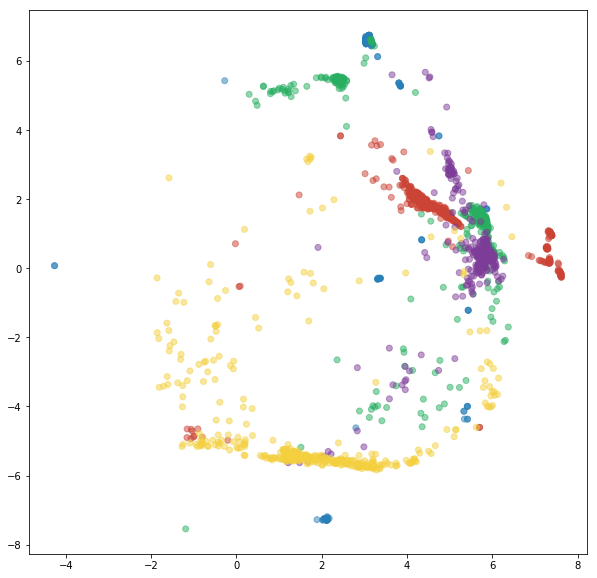
\includegraphics[scale=0.15]{P1C5}
\end{figure}

\begin{figure}
\centering
\begin{minipage}{.5\textwidth}
  \captionof{figure}{Classical: Boccherini}
  \centering
  \includegraphics[scale=0.15]{P2C1}
  \label{fig:test1}
\end{minipage}%
\begin{minipage}{.5\textwidth}
  \captionof{figure}{Classical: Gluck}
  \centering
  \includegraphics[scale=0.15]{P2C2}
  \label{fig:test2}
\end{minipage}
\end{figure}

\begin{figure}
\centering
\begin{minipage}{.5\textwidth}
  \captionof{figure}{Classical: Haydn}
  \centering
  \includegraphics[scale=0.15]{P2C3}
  \label{fig:test1}
\end{minipage}%
\begin{minipage}{.5\textwidth}
  \captionof{figure}{Classical: Mozart}
  \centering
  \includegraphics[scale=0.15]{P2C4}
  \label{fig:test2}
\end{minipage}
\end{figure}

\begin{figure}[h]
\caption{Classical: Salieri}
\centering
\includegraphics[scale=0.15]{P2C5}
\end{figure}

\begin{figure}
\centering
\begin{minipage}{.5\textwidth}
  \captionof{figure}{19th Century: Beethoven}
  \centering
  \includegraphics[scale=0.15]{P3C1}
  \label{fig:test1}
\end{minipage}%
\begin{minipage}{.5\textwidth}
  \captionof{figure}{19th Century: Clementi}
  \centering
  \includegraphics[scale=0.15]{P3C2}
  \label{fig:test2}
\end{minipage}
\end{figure}

\begin{figure}
\centering
\begin{minipage}{.5\textwidth}
  \captionof{figure}{19th Century: Gossec}
  \centering
  \includegraphics[scale=0.15]{P3C3}
  \label{fig:test1}
\end{minipage}%
\begin{minipage}{.5\textwidth}
  \captionof{figure}{19th Century: Kalliwoda}
  \centering
  \includegraphics[scale=0.15]{P3C4}
  \label{fig:test2}
\end{minipage}
\end{figure}

\begin{figure}[h]
\caption{19th Century: Rubinstein}
\centering
\includegraphics[scale=0.15]{P3C5}
\end{figure}

\begin{figure}
\centering
\begin{minipage}{.5\textwidth}
  \captionof{figure}{Romantic: Dvorak}
  \centering
  \includegraphics[scale=0.15]{P4C1}
  \label{fig:test1}
\end{minipage}%
\begin{minipage}{.5\textwidth}
  \captionof{figure}{Romantic: Mendelssohn}
  \centering
  \includegraphics[scale=0.15]{P4C2}
  \label{fig:test2}
\end{minipage}
\end{figure}

\begin{figure}
\centering
\begin{minipage}{.5\textwidth}
  \captionof{figure}{Romantic: Schubert}
  \centering
  \includegraphics[scale=0.15]{P4C3}
  \label{fig:test1}
\end{minipage}%
\begin{minipage}{.5\textwidth}
  \captionof{figure}{Romantic: Schumann}
  \centering
  \includegraphics[scale=0.15]{P4C4}
  \label{fig:test2}
\end{minipage}
\end{figure}

\begin{figure}[h]
\caption{Romantic: Tchaikovsky}
\centering
\includegraphics[scale=0.15]{P4C5}
\end{figure}

\begin{figure}
\centering
\begin{minipage}{.5\textwidth}
  \captionof{figure}{20th Cen: Antheil}
  \centering
  \includegraphics[scale=0.15]{P5C1}
  \label{fig:test1}
\end{minipage}%
\begin{minipage}{.5\textwidth}
  \captionof{figure}{20th Cen: Rachmaninoff}
  \centering
  \includegraphics[scale=0.15]{P5C2}
  \label{fig:test2}
\end{minipage}
\end{figure}

\begin{figure}
\centering
\begin{minipage}{.5\textwidth}
  \captionof{figure}{20th Cen: Rubbra}
  \centering
  \includegraphics[scale=0.15]{P5C3}
  \label{fig:test1}
\end{minipage}%
\begin{minipage}{.5\textwidth}
  \captionof{figure}{20th Cen: Shostakovich}
  \centering
  \includegraphics[scale=0.15]{P5C4}
  \label{fig:test2}
\end{minipage}
\end{figure}

\begin{figure}[h]
\caption{20th Cen: Stravinsky}
\centering
\includegraphics[scale=0.15]{P5C5}
\end{figure}

\begin{figure}[h]
\caption{All Symphonies Part 1}
\centering
\includegraphics[scale=0.08]{p1-2_allsymphonies}
\end{figure}

\begin{figure}[h]
\caption{All Symphonies Part 2}
\centering
\includegraphics[scale=0.08]{p2_allsymphonies}
\end{figure}

\begin{figure}[h]
\caption{All Symphonies Part 3}
\centering
\includegraphics[scale=0.08]{p3_symphonies}
\end{figure}

\begin{figure}[h]
\caption{All Symphonies Part 4}
\centering
\includegraphics[scale=0.08]{p4_allsymphonies}
\end{figure}

\begin{figure}[h]
\caption{All Symphonies Part 5}
\centering
\includegraphics[scale=0.08]{p5_allsymphonies}
\end{figure}
%%%%%%%%%%%%%%%%%%%%%%%%%%%%%%%%%%%%%%%%%%%%%%%%%%%%%%%%%%%%%%%%%%%%%%%%%%%%%%%%%%%%%%%%%%%%%%%%%%%%%%
%
%   Filename    : appendix_A.tex 
%
%   Description : This file is one of the appendices. 
%                 
%%%%%%%%%%%%%%%%%%%%%%%%%%%%%%%%%%%%%%%%%%%%%%%%%%%%%%%%%%%%%%%%%%%%%%%%%%%%%%%%%%%%%%%%%%%%%%%%%%%%%%

\textbf{\Huge Appendix G}
\bigskip

\textbf{\LARGE Symphony Title Map}

\bigskip
This section contains the title map for symphonies as was used in the research.

\includepdf[pages=-]{title_map.pdf}

\bibliography{myreferences}       %-- the file "myreferences.bib" is a sample bibliography (bib) from SIGGRAPH 
                                  %-- your job: **CREATE/EDIT** your own bibliography file  


\end{document}

